\documentclass[a4paper,11pt]{article}
\pdfoutput=1 % if your are submitting a pdflatex (i.e. if you have
             % images in pdf, png or jpg format)

\usepackage{jheppub} % for details on the use of the package, please
                     % see the JHEP-author-manual

\usepackage[T1]{fontenc} % if needed
\usepackage{tikz}
\usepackage{subcaption}
\usetikzlibrary{decorations.pathmorphing, arrows.meta, decorations.markings}
\usepackage{bbm}


\title{\boldmath Notes on Magnetic Monopoles}


%% %simple case: 2 authors, same institution
%% \author{A. Uthor}
%% \author{and A. Nother Author}
%% \affiliation{Institution,\\Address, Country}

% more complex case: 4 authors, 3 institutions, 2 footnotes
\author[]{Alonso Rodríguez Calleja}

% The "\note" macro will give a warning: "Ignoring empty anchor..."
% you can safely ignore it.

\affiliation[a]{Universidad de Valencia}

% e-mail addresses: one for each author, in the same order as the authors
\emailAdd{calleja4@alumni.uv.es}




\abstract{In this work, we bridge the fundamental theory of magnetic monopoles with contemporary experimental efforts. We first establish the mathematical necessity of monopoles via the Dirac Quantization Condition, progressing to their natural emergence as topological solitons in non-abelian gauge theories. This includes a detailed examination of the 't Hooft-Polyakov solution and the Standard Model's electroweak Cho-Maison monopole, along with the regularization schemes required to tame its divergent energy. Finally, we contextualize these theoretical models within the modern collider landscape. By detailing specialized detection methodologies, we summarize the current experimental constraints and the latest mass exclusion bounds.}



\begin{document} 
\maketitle
\flushbottom

\section{Dirac Quantization Condition}
\subsection{The Aharonov-Bohm effect}
Let us consider a spacetime evolution between two points $(t_a, x_a)$ and $(t_b, x_b)$, where $t_b > t_a$ and $x_i \in \mathbb{R}^3$. Between $x_a$ and $x_b$, the experimental setup features a double-slit screen (with slits $S_1$ and $S_2$) and an infinite solenoid. This solenoid produces a constant magnetic field strictly confined within a cylindrical region $\mathcal{D} \subseteq \mathbb{R}^3$. The whole setup is schematized as follows:

\begin{figure}[ht!]
    \centering
 

% Gradient Info
  
\tikzset {_cxwfksxb0/.code = {\pgfsetadditionalshadetransform{ \pgftransformshift{\pgfpoint{89.1 bp } { -108.9 bp }  }  \pgftransformscale{1.32 }  }}}
\pgfdeclareradialshading{_88ohik5i0}{\pgfpoint{-72bp}{88bp}}{rgb(0bp)=(1,1,1);
rgb(9.553571428571427bp)=(1,1,1);
rgb(25bp)=(0.8,0.8,0.8);
rgb(400bp)=(0.8,0.8,0.8)}
\tikzset{every picture/.style={line width=0.75pt}} %set default line width to 0.75pt        

\begin{tikzpicture}[x=0.75pt,y=0.75pt,yscale=-1,xscale=1]
%uncomment if require: \path (0,300); %set diagram left start at 0, and has height of 300

%Straight Lines [id:da18832869393626284] 
\draw    (177.29,105) -- (177.29,142.88) ;
%Straight Lines [id:da7682554576089895] 
\draw    (177.29,157.47) -- (177.29,195.35) ;
%Straight Lines [id:da31020950872564756] 
\draw    (177.54,210.45) -- (177.54,248.33) ;
%Curve Lines [id:da656979146831886] 
\draw [blue!60!black ,draw opacity=1 ]   (114.1,176.41) .. controls (150.03,163.36) and (201.58,273.42) .. (351.77,176.67) ;
\draw [shift={(236.61,216.85)}, rotate = 181.7] [fill=blue!60!black  ,fill opacity=1 ][line width=0.08]  [draw opacity=0] (6.25,-3) -- (0,0) -- (6.25,3) -- cycle    ;
%Curve Lines [id:da438677995287575] 
\draw [blue!60!black ,draw opacity=1 ]   (114.1,176.41) .. controls (172.34,149.02) and (233.8,98.86) .. (351.77,176.67) ;
\draw [shift={(237.6,135.1)}, rotate = 179.93] [fill=blue!60!black  ,fill opacity=1 ][line width=0.08]  [draw opacity=0] (6.25,-3) -- (0,0) -- (6.25,3) -- cycle    ;
%Shape: Ellipse [id:dp7238113732545107] 
\draw  [fill={rgb, 255:red, 0; green, 0; blue, 0 }  ,fill opacity=1 ] (348.05,176.67) .. controls (348.05,174.55) and (349.71,172.83) .. (351.77,172.83) .. controls (353.82,172.83) and (355.48,174.55) .. (355.48,176.67) .. controls (355.48,178.79) and (353.82,180.51) .. (351.77,180.51) .. controls (349.71,180.51) and (348.05,178.79) .. (348.05,176.67) -- cycle ;
%Shape: Ellipse [id:dp0006365999759496699] 
\path  [shading=_88ohik5i0,_cxwfksxb0] (246.93,173.34) .. controls (246.93,162.74) and (255.26,154.14) .. (265.52,154.14) .. controls (275.79,154.14) and (284.11,162.74) .. (284.11,173.34) .. controls (284.11,183.94) and (275.79,192.54) .. (265.52,192.54) .. controls (255.26,192.54) and (246.93,183.94) .. (246.93,173.34) -- cycle ; % for fading 
 \draw   (246.93,173.34) .. controls (246.93,162.74) and (255.26,154.14) .. (265.52,154.14) .. controls (275.79,154.14) and (284.11,162.74) .. (284.11,173.34) .. controls (284.11,183.94) and (275.79,192.54) .. (265.52,192.54) .. controls (255.26,192.54) and (246.93,183.94) .. (246.93,173.34) -- cycle ; % for border 

%Shape: Ellipse [id:dp8280390261989105] 
\draw   (246.93,173.34) .. controls (246.93,162.74) and (255.26,154.14) .. (265.52,154.14) .. controls (275.79,154.14) and (284.11,162.74) .. (284.11,173.34) .. controls (284.11,183.94) and (275.79,192.54) .. (265.52,192.54) .. controls (255.26,192.54) and (246.93,183.94) .. (246.93,173.34) -- cycle ;
%Shape: Ellipse [id:dp058429493810445265] 
\draw   (258.46,173.34) .. controls (258.46,169.31) and (261.62,166.04) .. (265.52,166.04) .. controls (269.42,166.04) and (272.58,169.31) .. (272.58,173.34) .. controls (272.58,177.37) and (269.42,180.63) .. (265.52,180.63) .. controls (261.62,180.63) and (258.46,177.37) .. (258.46,173.34) -- cycle ;
%Shape: Ellipse [id:dp6775830231507322] 
\draw  [fill={rgb, 255:red, 0; green, 0; blue, 0 }  ,fill opacity=1 ] (263.66,173.34) .. controls (263.66,172.28) and (264.49,171.42) .. (265.52,171.42) .. controls (266.55,171.42) and (267.38,172.28) .. (267.38,173.34) .. controls (267.38,174.4) and (266.55,175.26) .. (265.52,175.26) .. controls (264.49,175.26) and (263.66,174.4) .. (263.66,173.34) -- cycle ;
%Shape: Ellipse [id:dp5571197210257238] 
\draw  [fill={rgb, 255:red, 0; green, 0; blue, 0 }  ,fill opacity=1 ] (110.38,176.41) .. controls (110.38,174.29) and (112.04,172.57) .. (114.1,172.57) .. controls (116.15,172.57) and (117.81,174.29) .. (117.81,176.41) .. controls (117.81,178.53) and (116.15,180.25) .. (114.1,180.25) .. controls (112.04,180.25) and (110.38,178.53) .. (110.38,176.41) -- cycle ;

% Text Node
\draw (235,220.7) node [anchor=north west][inner sep=0.75pt]  [blue!60!black  ,opacity=1 ]  {$\gamma _{2}$};
% Text Node
\draw (235,115.34) node [anchor=north west][inner sep=0.75pt]  [blue!60!black  ,opacity=1 ]  {$\gamma _{1}$};
% Text Node
\draw (285,160) node [anchor=north west][inner sep=0.75pt]    {$B$};
% Text Node
\draw (230,150) node [anchor=north west][inner sep=0.75pt]    {$\mathcal{D}$};
% Text Node
\draw (148,124.81) node [anchor=north west][inner sep=0.75pt]    {$S_{1}$};
% Text Node
\draw (148,204.67) node [anchor=north west][inner sep=0.75pt]    {$S_{2}$};
% Text Node
\draw (90,140) node [anchor=north west][inner sep=0.75pt]    {$( t_{a} ,x_{a})$};
% Text Node
\draw (328,140) node [anchor=north west][inner sep=0.75pt]    {$( t_{b} ,x_{b})$};


\end{tikzpicture}
\caption{Schematic representation of the experimental setup. A charged point particle propagates from an initial spacetime point $(t_a, x_a)$ to a final point $(t_b, x_b)$, passing through two slits, $S_1$ and $S_2$. An infinite solenoid, which produces a constant magnetic field $\boldsymbol{B}$ strictly confined within a cylindrical region $\mathcal{D}$.}
\label{expAB}
\end{figure}

From the perspective of non-relativistic quantum mechanics, the wavefunction describing a point particle propagates from $(t_a, x_a)$ to $(t_b, x_b)$ via the integral equation:
\begin{equation}
    \Psi(t_b,\boldsymbol x_b) = \int_{\mathbb{R}^3} d^3 \boldsymbol x'\ K( \boldsymbol x_b, t_b;  \boldsymbol x',t_a) \Psi(t_a,\boldsymbol x')\ ,
\end{equation}
where $K$ represents the kernel (or Green's function) of the Schrödinger operator. Within Feynman's path integral formulation, this kernel is constructed by summing over all possible trajectories, weighting each by the phase factor $\exp\left\{\frac{i}{\hbar} S[x(t)]\right\}$. Crucially, even though the magnetic field $\boldsymbol B=\boldsymbol 0$ for all $\boldsymbol x \in \mathbb{R}^3 \setminus \mathcal{D}$, the vector potential $A$ (satisfying $\boldsymbol \nabla \times \boldsymbol A = \boldsymbol B$) is non-vanishing in the region outside the solenoid. For a massive point particle with electric charge $q$, its dynamics are governed by the action functional:
\begin{equation}
    S = \int_{t_a}^{t_b} dt \left\{ \frac{m}{2}\dot{\boldsymbol x}^2 - \frac{q}{c}\dot{\boldsymbol{x}}\cdot\boldsymbol{A} \right\}\ ,
\end{equation}
note that a partial integration of the charged term showcases the fact that such term is path-dependent. With this in mind, the propagator naturally splits into contributions from paths passing through $S_1$ and $S_2$:
\begin{equation}
    \Psi(t_b, \boldsymbol x_b) =  \int_{\mathbb{R}^3} d^3  \boldsymbol x\ \left[K_1( \boldsymbol x_b, t_b;  \boldsymbol x, t_a) +  K_2( \boldsymbol x_b, t_b; \boldsymbol x, t_a) \right] \Psi(t_a, \boldsymbol x)\ ,
\end{equation}
where $K_1$ and $K_2$ describe the contributions from paths passing through $S_1$ and $S_2$, respectively. Furthermore, each kernel admits an additional decomposition based on the number of times a path loops around the solenoid region $\mathcal{D}$. Consider two paths $\gamma_1$ and $\gamma_2$ winding the solenoid the same number of times. Then, their phase difference is given by:
\begin{equation}
    \int_{\gamma_1} d\boldsymbol{x}\cdot\boldsymbol{A} - \int_{\gamma_2} d\boldsymbol{x}\cdot\boldsymbol{A} = \oint_{\gamma_1 \cup \gamma_2} d\boldsymbol{x}\cdot\boldsymbol{A} = \int_{\partial^{-1}(\gamma_1 \cup \gamma_2)} d\boldsymbol{S}\cdot(\boldsymbol\nabla \times \boldsymbol{A}) = \Phi_B W(\gamma_1 \cup \gamma_2)\ ,
\end{equation}
where $\Phi_B$ is the enclosed magnetic flux and $W \in \mathbb{Z}$ is a topological constant known as the winding number. Therefore, paths executing the same number of loops are homotopically equivalent. This allows the total kernel to be expressed as a sum over the free-particle kernels $K_W^{(0)}$ (evaluated as if $B=0$ everywhere), weighted by a topological phase:
 \begin{equation}
    K(\boldsymbol x_b, t_b; \boldsymbol x_a, t_a) = \sum_{W \in \mathbb{Z}} e^{i \frac{W q \Phi_B}{\hbar c}} \left( K_{1,W}^{(0)} + K_{2,W}^{(0)} \right)= \sum_{W \in \mathbb{Z}} e^{i \frac{W q \Phi_B}{\hbar c}} K_W^{(0)}\ .
 \end{equation}
Hence, the emergence of these relative phases, which are integer multiples of $q\Phi_B / \hbar c$, reflects the physical role of the vector potential in quantum theory. This is the so-called Aharonov-Bohm (AB) effect \cite{AharonovBohm1959}.

Now, let us take the specific limit where the solenoid's cross-section tends to zero ($\mathcal{D} \to \{ \text{line} \}$) and the experimental setup is centered around one endpoint of this line. The magnetic flux emanating from this point becomes:
 \begin{equation}
    \Phi_B = \int d\boldsymbol{S}\cdot\boldsymbol{B} = 4\pi g\ ,
 \end{equation}
 for some real constant $g$, which in total analogy with Gauss's law, can be understood as the charge of a \textit{magnetic monopole}. In this limit, the thin line is called the \textit{Dirac string} and should have no physical effect in the theory. Because the Dirac string is an unphysical mathematical artifact, its presence must have no physical effect on the quantum theory. The only way to reconcile this unobservability with the AB effect is to demand that the string induces a trivial quantum phase:
 \begin{equation}
    \exp\left\{ \frac{i W q \Phi_B}{\hbar c} \right\} = 1 \iff \frac{W q \Phi_B}{\hbar c} = 2\pi n, \quad n \in \mathbb{N}\ .
 \end{equation}
 Setting $W=1$ for a single topological loop yields the \textit{Dirac Quantization Condition} (DQC) \cite{Dirac1931}:
 \begin{equation}
    q g = \frac{n}{2} \hbar c, \quad n \in \mathbb{N}\ .
 \end{equation}

Lastly, it is important to point out that all of these computations rely on the impossibility of paths crossing $\mathcal{D}$. Mathematically, this means the space $\mathbb{R}^3 \setminus \mathcal{D}$ is not simply connected, possessing a non-trivial first homotopy group ($\Pi_1(\mathbb{R}^3 \setminus \mathcal{D}) =\mathbb{Z}$). By contrast, the existence of the point-like monopole itself is a consequence of removing a singular origin from spacetime, which makes the second homotopy group non-trivial ($\Pi_2(\mathbb{R}^3 \setminus \{0\}) \cong \mathbb{Z}$).

 \begin{figure}[ht!]
    \centering
    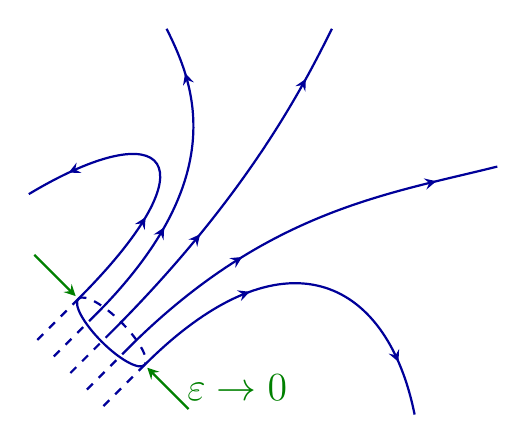
\begin{tikzpicture}[scale=0.7,
    >=stealth,
    % Define a style for the magnetic field lines with arrows along the path
    fieldline/.style={
        thick,
        draw=blue!60!black,
        postaction={decorate},
        decoration={
            markings,
            mark=at position 0.35 with {\arrow{>}},
            mark=at position 0.85 with {\arrow{>}}
        }
    }
]

% 1. Inner dashed lines (representing the Dirac string extending infinitely backwards)
\foreach \i/\j in {-0.6/0.6, -0.3/0.3, 0/0, 0.3/-0.3, 0.6/-0.6} {
    \draw[dashed, thick, blue!60!black] (\i, \j) -- ++(-0.8, -0.8);
}

% 2. Circular cross-section (viewed as an ellipse in perspective)
% The normal vector of the tube is roughly at 45 degrees, so we rotate the ellipse by -45
\begin{scope}[rotate=-45]
    % Back half of the cross-section (dashed)
    \draw[blue!60!black, thick, dashed] (-0.848, 0) arc (180:0:0.848 and 0.25);
    % Front half of the cross-section (solid)
    \draw[blue!60!black, thick] (-0.848, 0) arc (180:360:0.848 and 0.25);
\end{scope}

% 3. The magnetic field lines opening into a monopole
% Line 1 (Top-left): curves back on itself
\draw[fieldline] (-0.6, 0.6) .. controls (1.9, 3.1) and (1.0, 4.0) .. (-1.5, 2.5);
% Line 2 (Mid-left): sweeps up and left
\draw[fieldline] (-0.3, 0.3) .. controls (2.2, 2.8) and (1.5, 4.5) .. (1.0, 5.5);
% Line 3 (Center): sweeps straight up
\draw[fieldline] (0, 0)      .. controls (2.5, 2.5) and (3.5, 4.5) .. (4.0, 5.5);
% Line 4 (Mid-right): sweeps right
\draw[fieldline] (0.3, -0.3) .. controls (2.8, 2.2) and (5.0, 2.5) .. (7.0, 3.0);
% Line 5 (Bottom-right): sweeps down and right
\draw[fieldline] (0.6, -0.6) .. controls (3.1, 1.9) and (5.0, 1.0) .. (5.5, -1.5);

% 4. Epsilon parametrization arrows and label
% Top arrow pointing to the upper-left edge
\draw[<-, thick, green!50!black] (-0.65, 0.65) -- (-1.4, 1.4);
% Bottom arrow pointing to the lower-right edge
\draw[<-, thick, green!50!black] (0.65, -0.65) -- (1.4, -1.4);

% Epsilon label
\node[green!50!black, anchor=north west] at (1.2, -0.6) {\Large $\varepsilon \to 0$};

\end{tikzpicture}
\caption{Conceptual representation of a Dirac string. As the cross-sectional radius of the solenoid approaches zero ($\varepsilon \to 0$), it collapses into an infinitely thin, unobservable flux tube that feeds magnetic flux into the origin}
\label{diracstring}
 \end{figure}
 \textbf{Remark:} throughout the whole paper, we will switch between CGS units and natural units ($\hbar=c=4\pi \epsilon_0=1$). Concerning the electric charge $e$, recall that the fine-structure constant in CGS unit was:
 \begin{equation}
    \alpha_e=\dfrac{e^2}{\hbar c}\approx \frac{1}{137}\ ,
 \end{equation}
 from this expression, it is clear that the mapping $e^2\mapsto e^2/\hbar c$ relates CGS and natural units.
 \subsection{Vector potential for a magnetic monopole}
 In the previous section, we observed the fundamental role of the magnetic vector potential in the quantum theory and its deep relationship with magnetic monopoles. This, however, introduces an apparent contradiction: the very existence of a global vector potential $\boldsymbol A$ strictly requires a divergence-free magnetic field ($\boldsymbol \nabla \cdot \boldsymbol B = 0$), which seems incompatible with a point-like magnetic charge. 
 
 To resolve this tension, we can construct a naïve vector potential for the monopole. In spherical coordinates, such potential can be given by:
\begin{equation}
 \boldsymbol{A}^N = \frac{g}{r} \frac{(1 - \cos\theta)}{\sin\theta} \hat{\boldsymbol \varphi}
\end{equation}
Indeed, the use of the curl in spherical coordinates confirms that it generates the correct monopole field:
\begin{equation}
    \boldsymbol{\nabla} \times \boldsymbol{A}^N = \frac{1}{r\sin\theta} \partial_\theta (\sin\theta A^N_\varphi) \hat{\boldsymbol r} = g \frac{ \hat{\boldsymbol r}}{r^2}
\end{equation}
However, $\boldsymbol A^{(N)}$ possesses two distinct singularities. The first is the expected divergence at $r=0$, corresponding to the point-like nature of the source. The second is a novel half-line singularity located at $\theta=\pi$, which extends from the origin down to the south pole, which is precisely the Dirac string. Note that the potential is completely well-behaved at the north pole ($\theta=0$). To treat this singularity formally, we evaluate the curl of $\boldsymbol A^{(N)}$ in a distributional sense. For that, let us define a functional acting on a smooth test function $\boldsymbol T(\boldsymbol x)$:
 \begin{equation}
    I_{\boldsymbol{T}}[\boldsymbol{\nabla} \times \boldsymbol{A}^{(N)}] \equiv \int_{\mathbb{R}^3} d^3 \boldsymbol x\  \boldsymbol{A}^{(N)} \cdot [\boldsymbol{\nabla} \times \boldsymbol{T}(\boldsymbol{x})]
 \end{equation}
We regularize this integral by removing a tiny cylindrical region $\mathcal{D}_\epsilon$ of radius $\epsilon$ around the negative $z$-axis (as depicted in Figure \ref{poles}) and integrating by parts:
 \begin{figure}[ht!]
    \centering
    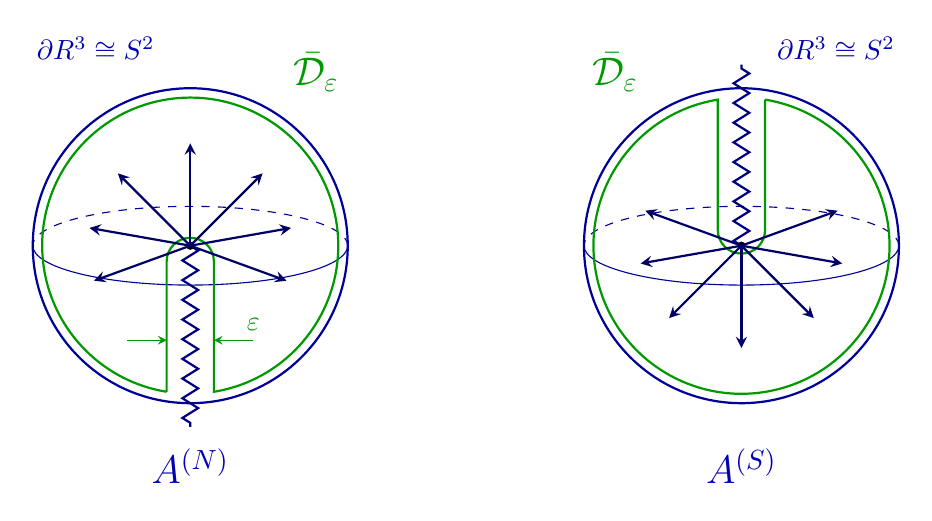
\begin{tikzpicture}
        % ==========================================
        % LEFT DIAGRAM: Vector Potential A^(N)
        % ==========================================
        \begin{scope}[shift={(0,0)}]
            % Outer Sphere (Boundary)
            \draw [blue!60!black, thick] (0,0) circle (2);
            % Equator
            \draw [blue!60!black, dashed] (2,0) arc (0:180:2 and 0.5);
            \draw [blue!60!black] (-2,0) arc (180:360:2 and 0.5);

            % Green Region \bar{D}_\varepsilon
            % Calculates the intersection at x=0.3, r=1.88 -> y=-1.855 (angle approx -80.8 deg)
            \draw [green!60!black, thick]
                (-0.3, -1.855) -- (-0.3, -0.2)
                arc[start angle=180, end angle=0, radius=0.3]
                -- (0.3, -1.855)
                arc[start angle=-80.8, end angle=260.8, radius=1.88];

            % Dirac String (Zigzag line along negative z-axis)
            \draw [decorate, decoration={zigzag, segment length=2.5mm, amplitude=1mm}, blue!50!black, thick] (0,0) -- (0,-2.3);

            % Origin Point and r=0 label
            \fill (0,0) circle (1.5pt);
            \node [above left] at (-0.1, 0.1) {};

            % Epsilon (\varepsilon) width markers
            \draw [->, green!60!black, >=stealth] (-0.8, -1.2) -- (-0.3, -1.2);
            \node [green!60!black] at (-1.0, -1.2) {\footnotesize };
            \draw [->, green!60!black, >=stealth] (0.8, -1.2) -- (0.3, -1.2);
            \node [green!60!black] at (0.8, -1.0) { $\varepsilon$};

            % Vector field arrows extending outward
            \foreach \a in {10, 45, 90, 135, 170, 200, 340} {
                \draw [->, blue!40!black, thick, >=stealth] (0,0) -- (\a:1.3);
            }

            % Labels
            \node [blue!70!black] at (-1.2, 2.5) {$\partial \mathbb{R}^3 \cong \mathbb{S}^2$};
            \node [green!60!black] at (1.6, 2.2) {\Large $\bar{\mathcal{D}}_\varepsilon$};
            \node [blue!70!black] at (0, -2.8) {\Large ${\boldsymbol{A}}^{(N)}$};
        \end{scope}

        % ==========================================
        % RIGHT DIAGRAM: Vector Potential A^(S)
        % ==========================================
        \begin{scope}[shift={(7,0)}]
            % Outer Sphere (Boundary)
            \draw [blue!60!black, thick] (0,0) circle (2);
            % Equator
            \draw [blue!60!black, dashed] (2,0) arc (0:180:2 and 0.5);
            \draw [blue!60!black] (-2,0) arc (180:360:2 and 0.5);

            % Green Region \bar{D}_\varepsilon
            % Calculates the intersection at x=-0.3, r=1.88 -> y=1.855 (angle approx 99.2 deg)
            \draw [green!60!black, thick]
                (0.3, 1.855) -- (0.3, 0.2)
                arc[start angle=360, end angle=180, radius=0.3]
                -- (-0.3, 1.855)
                arc[start angle=99.2, end angle=440.8, radius=1.88];

            % Dirac String (Zigzag line along positive z-axis)
            \draw [decorate, decoration={zigzag, segment length=2.5mm, amplitude=1mm}, blue!50!black, thick] (0,0) -- (0,2.3);

            % Origin Point and r=0 label
            \fill (0,0) circle (1.5pt);
            \node [right] at (0.4, 0.4) {};

            % Vector field arrows extending outward
            \foreach \a in {190, 225, 270, 315, 350, 160, 20} {
                \draw [->, blue!40!black, thick, >=stealth] (0,0) -- (\a:1.3);
            }

            % Labels
            \node [blue!70!black] at (1.2, 2.5) {$\partial \mathbb{R}^3 \cong \mathbb{S}^2$};
            \node [green!60!black] at (-1.6, 2.2) {\Large $\bar{\mathcal{D}}_\varepsilon$};
            \node [blue!70!black] at (0, -2.8) {\Large ${\boldsymbol{A}}^{(S)}$};
        \end{scope}
    \end{tikzpicture}
    \caption{Magnetic monopole vector potentials and their corresponding Dirac strings. The complementary region $\bar{\mathcal{D}}_\varepsilon$ is emphasized in green.}
    \label{poles}
\end{figure}
 \begin{align}
    \begin{split}
         I_{\boldsymbol{T}}[\boldsymbol{\nabla} \times \boldsymbol{A}^{(N)}] &= \lim_{\varepsilon \to 0} \left\{ \int_{\bar{\mathcal D}_\varepsilon} d^3\boldsymbol x \left( \boldsymbol{T} \cdot (\boldsymbol{\nabla} \times \boldsymbol{A}^{(N)}) - \boldsymbol{\nabla} \cdot (\boldsymbol{A}^{(N)} \times \boldsymbol{T}) \right) \right\}\\
         &\equiv \lim_{\varepsilon \to 0} (a_1(\varepsilon) + a_2(\varepsilon))
    \end{split}
 \end{align}
The bulk term $a_1(\epsilon)$ behaves regularly and yields the standard monopole field:
 \begin{equation}
    \lim_{\varepsilon\to 0}a_1(\varepsilon) = \int_{\mathbb{R}^3} d^3\boldsymbol x\ \boldsymbol{T}(\boldsymbol{x}) \cdot g \frac{\hat{\boldsymbol r}}{r^2}\ .
 \end{equation}
 For the boundary term $a_2(\epsilon)$, we express $\boldsymbol A^{(N)}$ in cylindrical coordinates $(\rho, \varphi, z)$. Near the string ($\epsilon \to 0$), we have $r = \sqrt{\rho^2 + z^2} \approx -z$ (since $z < 0$). The potential approximates to $\boldsymbol A^{(N)} \approx (2g/\rho)\hat{\boldsymbol \varphi}$. Applying the divergence theorem to evaluate the flux through the inner cylindrical boundary with the measure $d^2\boldsymbol x = -\hat{\boldsymbol \rho}\epsilon \, d\varphi \, dz$, we find:
 \begin{align}
    \begin{split}
        \lim_{\varepsilon \to 0} a_2(\varepsilon) &= \int_{\mathbb{R}^-} dz \int_0^{2\pi} d\phi\ \boldsymbol{T} \cdot \left( \frac{2g}{\varepsilon} \cdot \varepsilon \right) \hat{\boldsymbol z}= \int_{\mathbb{R}^-} dz\  \boldsymbol{T} \cdot (4\pi g \hat{\boldsymbol z})\\
        &=\int_{\mathbb{R}^3} d^3\boldsymbol x\ \boldsymbol{T} \cdot (4\pi g \delta(x) \delta(y) \theta(-z) \hat{\boldsymbol z})\ .
    \end{split}
 \end{align}
Combining these results, the rigorously defined, regularized magnetic field is obtained through the functional:
 \begin{equation}
    I_{\boldsymbol{T}}[\boldsymbol{\nabla} \times \boldsymbol{A}^{(N)}] = \int_{\mathbb{R}^3} d^3\boldsymbol x\ \boldsymbol{T}(\boldsymbol x) \cdot \left[ g \frac{\hat{\boldsymbol r}}{r^2} + 4\pi g \delta(x) \delta(y) \theta(-z) \hat{\boldsymbol z}\ , \right]
 \end{equation}
 hence:
 \begin{equation}
    \boldsymbol{B}_{\text{reg.}} = g \frac{\hat{\boldsymbol r}}{r^2} + 4\pi g \delta(x) \delta(y) \theta(-z) \hat{\boldsymbol z}\ .
 \end{equation}
Note that the second term represents an infinite solenoid feeding magnetic flux into the origin, as expected from the Dirac string. By taking the divergence of this regularized field, we find:
 \begin{equation}
    \boldsymbol{\nabla} \cdot \boldsymbol{B}_{\text{reg.}} = 4\pi g \delta^{(3)}(\boldsymbol{x})(1 - 1)=0\ ,
 \end{equation}
showing that the string flux perfectly cancels the monopole source flux, mathematically satisfying Maxwell's equations everywhere.

 An equally valid choice of vector potential places the string along the positive $z$-axis ($\theta=0$), leaving the south pole regular:
 \begin{equation}
    \boldsymbol{A}^{(S)} = - g \frac{(1 + \cos\theta)}{r\sin\theta} \hat{\boldsymbol \varphi}\ .
 \end{equation}
 The relation between $\boldsymbol{A}^{(N)}$ and $\boldsymbol{A}^{(S)}$ is merely a gauge transformation:
 \begin{equation}
    A^{(N)}_\varphi - A^{(S)}_\varphi = \frac{1}{r\sin\theta} \partial_\varphi (2g\varphi) = \hat{\boldsymbol \varphi} \cdot \boldsymbol{\nabla}(2g\varphi)\equiv \hat{\boldsymbol \varphi} \cdot \boldsymbol{\nabla}\Lambda  \quad (\theta \neq 0, \pi)\ .
 \end{equation}
Because the physical wave-function must remain single-valued, the quantum phase shift induced by evaluating the gauge parameter $\Lambda(\varphi)$ around a full $2\pi$ rotation must be a multiple of $2\pi$. Since $\Lambda(2\pi) - \Lambda(0) = 4\pi g$, we demand:
 \begin{equation}
    \frac{e}{\hbar} 4\pi g = 2\pi n \implies eg = \frac{n}{2} \hbar\ ,
 \end{equation}
 retrieving the DQC.
 
 Finally, while it initially appears that a magnetic monopole inevitably requires a Dirac string, its location is arbitrary (dependent solely on the choice of potential). Recognizing this, Wu and Yang provided a solution \cite{WuYang1975}. They defined the piecewise vector potential:
 \begin{equation}
    A_\varphi = \begin{cases} A_\varphi^{(N)}, &  \theta \in (0, \pi/2)\ , \\ A_\varphi^{(S)}, &  \theta \in (\pi/2, \pi) \ ,\end{cases}
 \end{equation}
 which is smooth over the whole $\mathbb R^3$. Then, by denoting the northern hemisphere as $\mathbb R^N$ and the southern as $\mathbb R^S$ (note that $\partial \mathbb R^N=-\partial \mathbb R^S=\mathbb S^1$), they evaluated the magnetic flux over a 2-sphere:
 \begin{align}
    \begin{split}
        \Phi_B &= \oint_{\partial \mathbb R^N} d\boldsymbol{x} \cdot \boldsymbol{A}^{(N)} + \oint_{\partial \mathbb R^S} d\boldsymbol{x} \cdot \boldsymbol{A}^{(S)}\\
        &= \oint_{\mathbb S^1} d\boldsymbol{x} \cdot \boldsymbol{A}^{(N)} - \oint_{\mathbb S^1} d\boldsymbol{x} \cdot \boldsymbol{A}^{(S)} = \int_0^{2\pi} d\varphi \, \partial_\varphi (2g\varphi) = 4\pi g\ .
    \end{split}
 \end{align}
Demonstrating that the Dirac string is not a physical object, but just a consequence of an unwise choice of coordinates. Alternatively, the Dirac string is the manifestation of the topological impossibility of covering a 2-sphere with a single, non-singular coordinate chart \cite{Nakahara2003}.
\section{Monopoles in non-abelian gauge theories}
In the previous section, we derived how the existence of monopoles implies the quantization of electric charge, a well-known phenomenon observed in nature. In that sense, Dirac's arguments can be understood as consistent with quantum electrodynamics. The purpose of this section is not only to demonstrate that monopoles are classical predictions of certain gauge theories, but also to show that specific properties of these monopoles are computable within these theories.
 \subsection{'t Hooft–Polyakov monopole}
The simplest theoretical framework accommodating magnetic monopoles is an SU(2) gauge theory coupled to a scalar triplet (the Higgs field), $\phi^a$ (where $a=1,2,3$), which transforms under the adjoint representation. The Lagrangian density for this system is:
\begin{equation}
    \mathcal{L} = -\frac{1}{4} F_{\mu\nu}^a F^{a\mu\nu} + \frac{1}{2} (D_\mu \phi^a)^2 - \frac{\lambda}{4} (\phi^a \phi^a - v^2)^2\ .
\end{equation}
where $v$ is the real-valued vacuum expectation value (VEV) and $\lambda > 0$ dictates the scalar self-coupling. The covariant derivative and the non-abelian curvature tensor are defined, respectively, as:
\begin{align}
     D_\mu \phi^a &= \partial_\mu \phi^a + \tilde{g} \varepsilon^{abc} A_\mu^b \phi^c\ ,\\
F_{\mu\nu}^a &= \partial_\mu A_\nu^a - \partial_\nu A_\mu^a + \tilde{g} \varepsilon^{abc} A_\mu^b A_\nu^c\ .
\end{align}
From these definitions, it is clear that the classical field equations are:
\begin{align}
      D_\mu F^{a\mu\nu} &= \tilde{g} \varepsilon^{abc} (D^\nu \phi^b) \phi^c\ , \\
 D_\mu D^\mu \phi^a &= - \lambda (\phi^b \phi^b) \phi^a + \lambda v^2 \phi^a\ .
\end{align}
Because we are specifically interested in magnetic monopole solutions, we must filter out the set of unwanted configurations. We achieve this by searching for static (time-independent) configurations that minimize the energy functional:
\begin{equation}\label{energyfunctional}
    E = \int_{\mathbb R^3} d^3\boldsymbol x \left\{ \frac{1}{4} F_{ij}^a F^{aij} + \frac{1}{2} (D_i \phi^a)(D^i \phi^a) + \frac{\lambda}{4} (\phi^a \phi^a - v^2)^2 \right\}\ .
\end{equation}
To find these static solutions, we work in the temporal (or Weyl) gauge ($A_{0}^{a}=0$) and propose the spherically symmetric \textit{Hedgehog ansatz}:
\begin{equation}\label{Hedgehogansatz}
    \phi^a(x) \equiv \frac{x^a}{r} F(r) \quad \text{and} \quad A_i^a \equiv \varepsilon^{aij} \frac{x^j}{r} W(r)\ .
\end{equation}
For the energy functional to remain finite, we must impose strict boundary conditions at the origin and at spatial infinity. At spatial infinity, the scalar field must settle into the vacuum, meaning $\phi^{a}\phi^{a}\rightarrow v^{2}$. Simultaneously, the kinetic energy must vanish, requiring the gauge field to drop to zero ($A_{i}^{a}\rightarrow0$). Translating these physical requirements to our radial functions yields:
\begin{equation}
    F(r) \xrightarrow{r\to\infty} v \quad \text{and} \quad W(r) \xrightarrow{r\to\infty} \frac{1}{r}\ .
\end{equation}
The boundary conditions around the origin will be specified once the energy functional is expressed in terms of both hedgehog fields. The covariant derivative then reads as:
\begin{align}
    \begin{split}
          D_i \phi^a &= \frac{\delta^{ia}}{r} F(r) \left[ 1 - \tilde{g} r W(r) \right] + \frac{x^a x^i}{r^2} \left[ F' - \frac{F}{r} + \tilde{g} W F \right]\\
           &\equiv \delta^{ia} A + \frac{x^a x^i}{r^2}B \quad (B = F' - A)\ .
    \end{split}
\end{align}
Thus, its square becomes:
\begin{equation}
    (D_i \phi^a)^2 = 3A^2 + B^2 + 2AB=2A^2 + (F')^2\ , 
\end{equation}
meaning that:
\begin{equation}
    \frac{1}{2} (D_i \phi^a)^2 = \frac{1}{2} (F'(r))^2 + \frac{F^2(r)}{r^2} (1 - r W \tilde{g})^2\ .
\end{equation}

On a similar fashion, the abelian term of the curvature tensor becomes:
\begin{equation}\label{abelianterm}
    \partial_i A_j^a - \partial_j A_i^a = 2 \varepsilon^{aji} \frac{W}{r} + \left( W' - \frac{W}{r} \right) \left\{ \varepsilon^{ajk} \frac{x^k x^i}{r^2} - \varepsilon^{aik} \frac{x^k x^j}{r^2} \right\}\ .
\end{equation}
Which can be further simplified by fully antisymmetrizing the term in brackets. Indeed, since:
\begin{equation}
    \varepsilon^{ajk} x^i - \varepsilon^{aik} x^j - \varepsilon^{ijk} x^a - \varepsilon^{aji} x^k = 0\Rightarrow \varepsilon^{ajk} x^i - \varepsilon^{aik} x^j = - \varepsilon^{aij} x^k + \varepsilon^{ijk} x^a\ ,
\end{equation}
the bracket term can be written as:
\begin{equation}
    \frac{x^k}{r^2} \left\{ - \varepsilon^{aij} x^k + \varepsilon^{ijk} x^a \right\} = - \varepsilon^{aij} + \frac{x^a x^k}{r^2} \varepsilon^{ijk}\ ,
\end{equation}
and thus (\ref{abelianterm}) can be expressed as:
\begin{equation}
     \partial_i A_j^a - \partial_j A_i^a = 2 \varepsilon^{aji} \frac{W(r)}{r} + \left( W' - \frac{W}{r} \right) \left( \varepsilon^{aji} + \frac{x^a x^k}{r^2} \varepsilon^{ijk} \right)\ .
\end{equation}
Regarding the non-abelian term, it easily reads as:
\begin{equation}
    \tilde{g} \varepsilon^{abc} A_i^b A_j^c = \tilde{g} \frac{x^k x^l}{r^2} \varepsilon^{abc} \varepsilon^{bik} \varepsilon^{cjl} W^2(r)= \tilde{g} \frac{x^k x^a}{r^2} \varepsilon^{ijk} W^2(r)\ .
\end{equation}
Hence:
\begin{align}
    \begin{split}
         F_{ij}^a &= \varepsilon^{aij} \left( -W' - \frac{W}{r} \right) + \varepsilon^{ijk} \frac{x^k x^a}{r^2} \left( W' - \frac{W}{r} + \tilde{g} W^2 \right)\\
                & \equiv \varepsilon^{aij} G_1 + \varepsilon^{ijk} \frac{x^k x^a}{r^2} G_2\ .
    \end{split}
\end{align}
and then:
\begin{align}
    \begin{split}
        + \frac{1}{4} (F_{ij}^a)^2 &= G_1^2 + \frac{1}{2} (G_1 + G_2)^2\\
                =& \frac{1}{r^2} (W'(r)r + W)^2 + \frac{1}{2} \left( \frac{W}{r} (2 - r W \tilde{g}) \right)^2\ .
    \end{split}
\end{align}

Therefore, the energy functional (\ref{energyfunctional}) is expressed in terms of the Hedgehog ansatz (\ref{Hedgehogansatz}) as:
\begin{align}\label{energyfunctional2}
    \begin{split}
        E = 4\pi \int_{\mathbb{R}^+} dr& \Big\{ \frac{r^2}{2} (F'(r))^2 + F^2 (1 - \tilde{g} r W)^2  \\
    &  + \frac{W^2}{2} (2 - r W \tilde{g})^2 + (W' r + W)^2 + \frac{\lambda}{4} r^2 (F^2 - v^2)^2 \Big\}\ .
    \end{split}
\end{align}
To ensure convergence at the origin, the fields must behave as $F(r) \sim r$ and $W(r) \sim r$ as $r \to 0$. On the other hand, the coupled Euler-Lagrange equations determining the profiles of $F(r)$ and $W(r)$ are obtained by demanding $\delta_{F}E=\delta_{W}E=0$:
\begin{align}
     F'' + \frac{2}{r} F' &= \frac{2F}{r^2} (1 - \tilde{g} r W)^2 + \lambda F (F^2 - v^2)\ ,\\
 W'' + \frac{2}{r} W' &= \frac{W}{r^2} (1 - \tilde{g} r W)(2 - \tilde{g} r W) - \frac{\tilde{g} F^2}{r} (1 - \tilde{g} r W)\ .
\end{align}

These equations must generally be solved numerically, as depicted in Figure \ref{HPprofiles}. \begin{figure}[ht!]
    \centering
    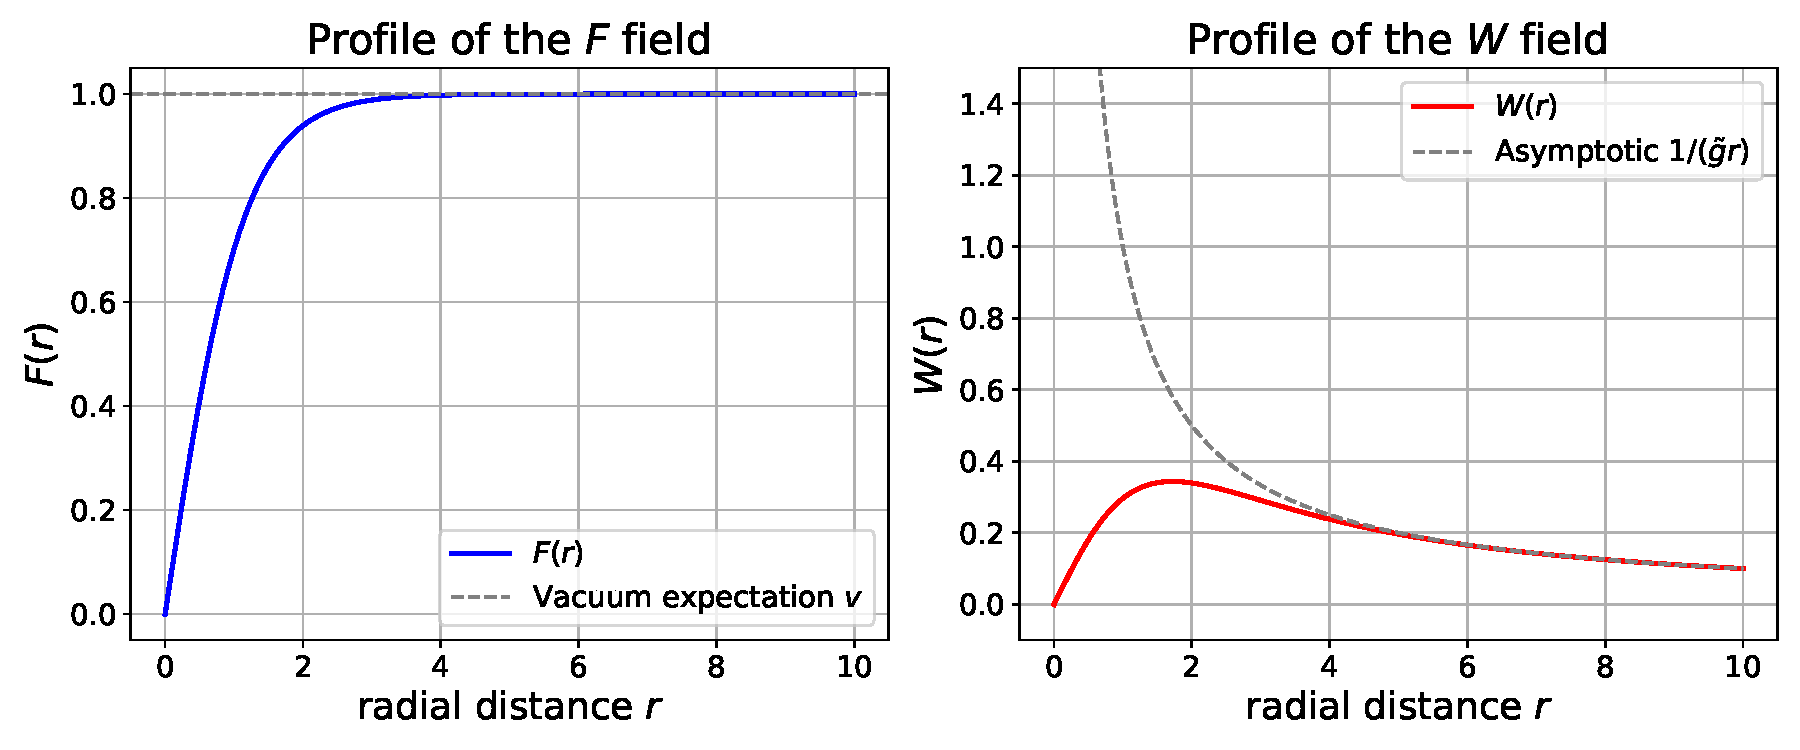
\includegraphics[scale=0.5]{HP_profiles.pdf}
    \caption{Numerical solutions for the radial profile functions $F(r)$ and $W(r)$ using the spherically symmetric Hedgehog ansatz. The coupled second-order differential equations are evaluated for the parameter choice $\lambda = v = \tilde{g} = 1$. As required by the boundary conditions, the scalar field profile $F(r)$ smoothly approaches the vacuum expectation value $v$ at spatial infinity, while the gauge field profile $W(r)$ converges to its asymptotic limit of $1/(\tilde{g}r)$.}
    \label{HPprofiles}
\end{figure}
 However, exact analytical solutions exist in the \textit{Bogomol'nyi-Prasad-Sommerfield (BPS) limit} \cite{PrasadSommerfield1975,Bogomolnyi1976}. This limit corresponds to taking $\lambda\to 0$, which physically represents the massless limit of the Higgs field while retaining a massive gauge boson. In this limit and for static configurations in the temporal gauge, eq. \ref{energyfunctional} becomes:
 \begin{equation}
    E=\int_{\mathbb R^3} d^3\boldsymbol x \left\{\frac{1}{2}(B_i^a)^2+\frac{1}{2}(D_i\phi^a)^2 \right\}=\int_{\mathbb R^3}d^3 \boldsymbol x \left\{\frac{1}{2}(B_i^a-D_i\phi^a)^2+D_i(B_i^a\phi^a) \right\}\ ,
\end{equation} 
with $B_i^a$ denoting the magnetic field. Within this limit, the second-order differential equations reduce to the first-order Bogomol'nyi equations ($B_{i}^{a}=D_{i}\phi^{a}$), leading to the analytical profiles:
\begin{align}
    F'(r)&=\frac{2W(r)}{r}(2-\tilde g r W(r))\ ,\\
    W'(r)+\frac{W(r)}{r}&=\frac{F(r)}{r}(1-\tilde g rW(r))\ .
\end{align}
Which are the natural replacement of the equations (2.22-2.23) within the BPS limit. However, this system of equations has an straightforward analytical solution given by the profiles:
\begin{align}
    F(r)&= \frac{1}{\tilde g r}\left(1-\frac{v\tilde g r}{\sinh(v\tilde g r)} \right) \ , \\
    W(r)&= v\text{coth}(v\tilde g r)-\frac{1}{\tilde g r}     \ .
\end{align}
For the sake of completitute, the profiles are represented in Figure \ref{profileBPS}.
\begin{figure}[ht!]
    \centering
    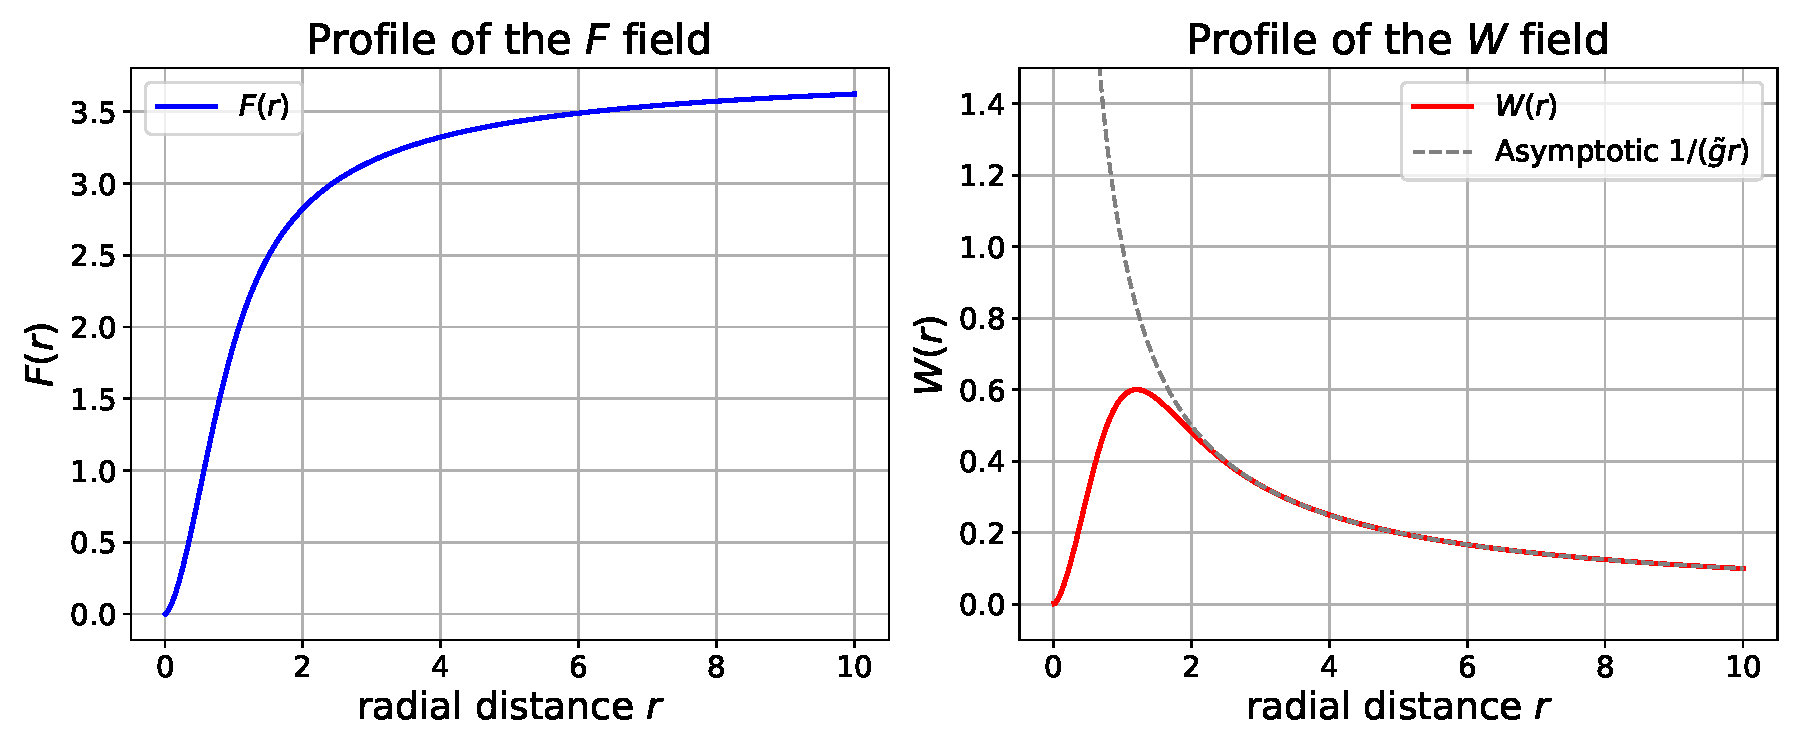
\includegraphics[scale=0.5]{HP_profilesBPS.pdf}
    \caption{Exact analytical solutions for the radial profiles $F(r)$ and $W(r)$ evaluated in the BPS limit with $\tilde g=1$.}
    \label{profileBPS}
\end{figure}
\subsubsection{Emergence of the monopole in the broken phase}
To meaningfully discuss a magnetic monopole, our theory must be mappped onto a $U(1)$ gauge theory. Because our original theory is $SU(2)$ invariant, we obtain this QED-like theory via Spontaneous Symmetry Breaking (SSB). For that, we define the normalized triplet in the internal space:
\begin{equation}
    \hat \phi^a\equiv \frac{\phi^a}{|\phi^a|}\ ,
\end{equation}
and the gauge-invariant electromagnetic curvature tensor:
\begin{equation}
    \mathcal F_{\mu\nu}\equiv \hat \phi^a\cdot F^a_{\mu\nu}-\frac{1}{\tilde g}\varepsilon^{abc}\hat \phi^a(D_\mu \hat \phi^b)(D_\nu \hat \phi ^b)=\partial_\mu(\hat\phi^a A^a_\nu)-\partial_\nu (\hat \phi^a A^a_\mu)\ .
\end{equation}
At spatial infinity, the resulting magnetic field $\mathcal{B}_{k}\equiv\frac{1}{2}\varepsilon_{ijk}\mathcal{F}^{ij}$ takes the form of a purely radial, point-like source:
\begin{equation}
    \lim_{r\to \infty} \mathcal B_k=\frac{1}{\tilde g}\frac{x_k}{r^3}\ ,
\end{equation}
Integrating this field over $\mathbb{S}_{\infty}^{2}$ gives the magnetic charge of the 't Hooft-Polyakov (HP) stringless monopole \cite{tHooft1974,Polyakov1974}:
\begin{equation}
    g_{\text{HP}}=\frac{1}{4\pi}\oint_{\mathbb S^2_\infty}d\Omega_2\ \boldsymbol{\hat r}r^2 \frac{\boldsymbol{\hat r}}{\tilde g r^2}=\frac{1}{\tilde g}\ .
\end{equation}
If we extend the DQC to this broken phase, noting that the charge of the gauge boson is $\tilde{g}$, we find that:
\begin{equation}
    q_{\text{HP}}g_{\text{HP}}=\hbar\ ,
\end{equation}
This implies that the HP monopole carries two Dirac magnetic quanta relative to the fundamental gauge boson. This factor of two arises because the scalar field transforms in the adjoint representation; a spinor representation would yield an additional factor of 1/2, recovering the standard $n=1$ DQC.

Finally, the mass of the monopole is bounded below by the topological term of the energy functional, a bound saturated exactly in the BPS limit ($M \ge \delta_{B}E$):
\begin{equation}
    M_{\text{BPS}}=\oint_{\mathbb S^2_\infty}d^2 \boldsymbol x\ n_i \phi^a B_i^a=v\oint_{\mathbb S^2_\infty}d^2\boldsymbol x \ n_i \mathcal B^i=\frac{4\pi v}{\tilde g}\ .
\end{equation}
Because the gauge boson mass generated during the $SU(2)\rightarrow U(1)$ breaking is $m_{GB}=v\tilde{g}$, the monopole mass can be elegantly written as:
\begin{equation}
    M_{\text{BPS}}=4\pi \frac{m_{\text{GB}}}{\tilde g^2}\ ,
\end{equation}
showcasing the deep relationship between the magnetic monopole and the Goldstone boson.
\subsubsection{Brief introduction to the monopole mass quantum corrections}
Classical observables naturally acquire quantum corrections as a consequence of field fluctuations around their classical configurations. The purpose of this subsection is to qualitatively analyze how the classical BPS mass, $M_{\text{BPS}}$, is modified at the one-loop (semiclassical) level \cite{FaddeevKorepin1978}. 

To achieve this, we focus on the $SU(2)$-invariant Lagrangian and expand the fields $(A_{\mu}^{a},\phi^{a})$ around the classical BPS solution:
\begin{align}
    A_\mu^a &= \bar{A}_\mu^a + \delta A_\mu^a\ , \\
    \phi^a &= \bar{\phi}^a + \delta \phi^a\ .
\end{align}
Next, we construct the quantum effective Lagrangian. For the gauge-fixing term, we choose:
\begin{equation}\mathcal{L}_{\text{gf}} = -\frac{1}{2\xi} f^a f^a \quad \text{with} \quad f^a = (\bar{D}_\mu \delta A^\mu)^a + \xi \tilde{g} \varepsilon^{abc} \bar{\phi}^b \delta \phi^c\ , \end{equation}
where $\overline{D}_{\mu}^{ab}$ represents the covariant derivative evaluated in the background:
\begin{equation}
    \bar{D}_\mu^{ab} = \delta^{ab} \partial_\mu - \tilde{g} \varepsilon^{abc} \bar{A}_\mu^c\ .
\end{equation}
Assuming $\xi=1$ (Feynman gauge) and denoting the infinitesimal parameters of the $\mathfrak{su}(2)$ algebra as $\{\omega^{a}\}$, the field transformations are:
\begin{align}
    \delta A_\mu^a &= \bar{D}_\mu \omega^a + \mathcal{O}(\omega^2)\ , \\
    \delta \phi^a &= -\tilde{g} \varepsilon^{abc} \bar{\phi}^b \omega^c + \mathcal{O}(\omega^2)\ .
\end{align}
Consequently, the ghost sector is given by:
\begin{equation}
    \mathcal{L}_{\text{gh.}} \equiv \bar{c}^a \left( \frac{\delta f^a}{\delta \omega^b} \right)\Bigg|_{\boldsymbol\omega=\boldsymbol 0} c^b = \bar{c}^a (\bar{D}_\mu \bar{D}^\mu)^{ab} - \tilde{g}^2 (\bar{\phi}^2 \delta^{ab} - \bar{\phi}^a \bar{\phi}^b) c^b\ .
\end{equation}
Assembling these components, the effective Lagrangian reads:
\begin{equation}
    \mathcal{L}_{\text{eff.}} = \frac{1}{2} \delta A_\mu^a \mathcal{M}^{ab\mu\nu} \delta A_\nu^b + \frac{1}{2} \delta \phi^a \mathcal{N}^{ab} \delta \phi^b + \bar{c}^a { \mathcal{O}^{ab} } c^b\ ,\end{equation}
where the respective differential operators are defined as:
\begin{align}
    \mathcal{M}^{\mu\nu ab} &= (\bar{D}_\alpha \bar{D}^\alpha)^{ab} \eta^{\mu\nu} + \tilde{g}^2 (\bar{\phi}^2 \delta^{ab} - \bar{\phi}^a \bar{\phi}^b) \eta^{\mu\nu} + 2 \tilde{g} \varepsilon^{abc} \bar{F}^{c\mu\nu }\ , \\
\mathcal{N}^{ab} &= (\bar{D}_\alpha \bar{D}^\alpha)^{ab} - \tilde{g}^2 (\bar{\phi}^2 \delta^{ab} - \bar{\phi}^a \bar{\phi}^b)\ , \\
\mathcal{O}^{ab} &= (-\bar{D}_\alpha \bar{D}^\alpha)^{ab} + \tilde{g}^2 (\bar{\phi}^2 \delta^{ab} - \bar{\phi}^a \bar{\phi}^b)\ ,
\end{align}
After performing the Gaussian integration, the one-loop partition function takes the form:
\begin{equation}\mathcal Z_{\text{1-loop}} \propto \frac{\det \mathcal{O}}{\sqrt{\det \mathcal{M} \det \mathcal{N}}}\ .\end{equation}
Now, the energy is related to the partition function through Feynman-Kac formula:
\begin{equation}E = \lim_{T \to \infty} \left(-\frac{1}{T} \log(\mathcal Z)\right)\ ,\end{equation}
thus, the mass corrections are obtained by subtracting the vacuum contribution of the classical configuration $(\phi,A)=(v,0)$:
\begin{equation}\Delta M = \lim_{T \to \infty} \left( -\frac{1}{T} \log\left(\frac{\mathcal Z}{\mathcal Z_0}\right) \right) \propto \frac{\det \mathcal{O} /\det \mathcal{O}_0}{\sqrt{\det \mathcal{M} / \det \mathcal{M}_0 \det \mathcal{N} / \det \mathcal{N}_0}}\ .\end{equation}

The main challenge with this formula is that it diverges, requiring a proper renormalization through a set of counterterms defined by a regularization scheme. For this system, zeta-function regularization emerges as the most natural choice \cite{KiselevSelivanov1989}.


\subsection{Cho-Maison (or electroweak) monopole in the Standard Model}
Having studied how the HP monopole arises from the coset space $SU(2)/U(1)$, it is natural to ask if an analogous monopole can appear in the broken phase of the Standard Model (SM), where the coset space is $SU(3)_c \times SU(2)_L \times U(1)_Y] / [SU(3)_c \times U(1)_{\text{EM}}$. Restricting our attention to the electroweak sector, there are two main topological aspects to consider. Firstly, the gauge group of the SM in both the unbroken and broken phases is compact, as the following isomorphisms hold:
\begin{equation}
    SU(2)_L \cong \mathbb S^3\quad ,\quad U(1)_Y \cong \mathbb S^1\quad,\quad   \frac{SU(2)_L \times U(1)_Y}{U(1)_{\text{EM}}} \cong \mathbb S^3\ .
\end{equation}
Note that this $\mathbb{S}^3$ structure is consistent with the emergence of three massive Goldstone degrees of freedom for the $W^{\pm}$ and $Z$ bosons. Secondly, $\mathbb{S}^3$ possesses a trivial second homotopy group ($\Pi_2(\mathbb{S}^3) = 0$), which formally forbids any strictly topological monopole solution. It is possible, however, to circumvent this constraint by focusing on a specific sector of the vacuum manifold. We start by introducing the normalized doublet:
\begin{equation}
    \hat{n} \equiv \frac{\Phi}{|\Phi|} \quad \text{such that}\quad \hat{n}^\dagger \hat{n}=1\ ,
\end{equation}
which lives in $\mathbb{S}^3$ and isolates the massive radial excitation of the Higgs field. We then define a 3-vector $\mathbf{m}$ related to $\hat{n}$ through the Pauli matrices:
\begin{equation}
    m^a = \hat{n}^\dagger \sigma^a \hat{n}, \quad a=1,2,3\ .
\end{equation}
This mapping preserves the normalization ($|\boldsymbol{m}|^2 = 1$), meaning $\boldsymbol{m} \in \mathbb{S}^2$. Unlike $\mathbb{S}^3$, the 2-sphere has a non-trivial second homotopy group, allowing a monopole solution to emerge. To track the physical limit where $|\Phi|\to 0$, recall the mapping $\mathbb{S}^2$ onto $\mathbb{C}\cup \{\infty\}\equiv \mathbb{C}\mathbb{P}^1 $ defined by the Riemann sphere.

To prove this quantitatively, we examine the electroweak sector of the SM Lagrangian:
\begin{equation}
    \mathcal{L} = |D_\mu H|^2 - \frac{1}{4} F_{\mu\nu}^a F^{a\mu\nu} - \frac{1}{4} B_{\mu\nu} B^{\mu\nu} - \frac{\lambda}{2} (H^\dagger H - \mu^2/\lambda)^2 \subset \mathcal{L}_{\text{SM}}\ ,
\end{equation}
with $\lambda, \mu^2 \in \mathbb{R}^+$ and the covariant derivative:
\begin{equation}
    D_\mu = \partial_\mu \mathbf 1_{2\times 2} - i \frac{g}{2} \sigma^a A_\mu^a - i \frac{g'}{2} B_\mu \mathbf{1}_{2\times 2}\ .
\end{equation}
In analogy to the normalized doublet, we propose the following spherically symmetric ansatz for the Higgs field:
\begin{equation}
    H = \frac{1}{\sqrt{2}} \rho(r) \xi(\theta, \varphi) \quad \text{such that} \quad \xi^\dagger \xi = 1\ ,
\end{equation}
then, denoting the vacuum expectation value as $\rho_0^2 = 2\mu^2/\lambda$ and applying the normalization condition, the Lagrangian reduces to:
\begin{equation}
    \mathcal{L} = \frac{1}{2}(\partial_\mu \rho)^2 + \frac{\rho^2}{2} |D_\mu \xi|^2 - \frac{1}{4}(F_{\mu\nu}^a)^2 - \frac{1}{4}(B_{\mu\nu})^2 - \frac{\lambda}{8}(\rho^2 - \rho_0^2)^2\ .
\end{equation}

To find a monopole configuration, we fix the 3-vector to be the radial unit vector $\hat{\boldsymbol r} \equiv \xi^\dagger \sigma \xi$. Along with the normalization condition, this uniquely determines the spinor:
\begin{equation}
\xi = \begin{pmatrix} \cos(\theta/2) \\ e^{i\varphi} \sin(\theta/2) \end{pmatrix}\ .
\end{equation}
For the non-abelian gauge fields, we utilize a slight modification of the HP ansatz:
\begin{equation}
    A_i^a = \frac{1}{g} \frac{\varepsilon^{aij}x^j}{r^2}(1-f(r)) \quad \text{with }\quad  A_0^a = 0\ ,
\end{equation}
and for the $U(1)_Y$ gauge field, we impose a Dirac string-like configuration:
\begin{equation}
    \boldsymbol{B} = \frac{1}{g'} \frac{1-\cos\theta}{r\sin\theta} \hat{\boldsymbol\varphi}\ .
\end{equation}
Regarding their boundary conditions, it is sufficient to fix at the origin $\rho=0$ and $f=1$, while fixing $\rho=v$ and $f=0$ at spatial infinity. Now we substitute these ansätze into the Lagrangian in order to build the energy functional. Firstly, note that:
\begin{equation}
    |D_\mu \xi|^2 = g^{\mu\nu} (D_\mu \xi)^\dagger (D_\nu \xi)= |D_r \xi|^2 + \frac{1}{r^2} |D_\theta \xi|^2 + \frac{1}{r^2\sin^2\theta} |D_\varphi \xi|^2\ ,
\end{equation}
since the gauge field is given in a cartesian basis, it is convenient to re-express its term within the covariant derivative as:
\begin{equation}
    -i \frac{g}{2} A_i^a = -i \frac{\varepsilon^{ail}}{2r^2} \sigma^a x^l (1-f(r))= i \frac{(1-f(r))}{2r} (\boldsymbol{\sigma}\times \hat{\boldsymbol r})_i\ ,
\end{equation}
and then use the relations:
\begin{align}
    \begin{split}
        (\boldsymbol{\sigma}\times\hat{\boldsymbol r})_r &= (\boldsymbol{\sigma}\times\hat{\boldsymbol r})\hat{r} = 0\ ,\\
        (\boldsymbol{\sigma}\times\hat{\boldsymbol r})_\theta &= (\boldsymbol{\sigma}\times\hat{r})\hat{\boldsymbol e}_\theta = r(\boldsymbol{\sigma}\times\hat{\boldsymbol r})\hat{\boldsymbol \theta} = r(\hat{\boldsymbol \varphi}\cdot\boldsymbol{\sigma})\ ,\\(\boldsymbol{\sigma}\times\hat{\boldsymbol r})_\varphi &= (\boldsymbol{\sigma}\times\hat{\boldsymbol r})\hat{\boldsymbol e}_\varphi = r\sin\theta (\boldsymbol{\sigma}\times\hat{\boldsymbol r})\hat{\boldsymbol \varphi} = -r\sin\theta (\boldsymbol{\sigma}\cdot\hat{\boldsymbol \theta})\ ,
    \end{split}
\end{align}
to find straightforwardly that:
\begin{equation}
    D_r \xi = 0, \quad |D_\theta \xi|^2 = |D_\varphi \xi|^2 = \frac{f^2(r)}{4}\ .
\end{equation}
Recycling the HP result for the $SU(2)$ curvature tensor, identifying $W(r) = (1-f(r))/r$, and calculating the $U(1)$ contribution yields:
\begin{equation}
    \frac{1}{4}(F_{ij}^a)^2 = \frac{(1-f^2)^2}{2g^2r^4} + \frac{(f')^2}{g^2r^2}, \quad \text{and} \quad \frac{1}{4}(B_{ij})^2 = \frac{1}{2(g')^2 r^4}\ .
\end{equation}
Hence, after integrating over the spatial volume $d^3\boldsymbol{x} = r^2 dr d\Omega_2$, the energy functional becomes:
\begin{equation}
    E= 4\pi \int_{\mathbb{R}^+} dr \left\{ (\rho'(r))^2 + \frac{\rho^2}{4} f^2(r) + \frac{(1-f^2)^2}{2g^2 r^2} + \frac{(f')^2}{g^2} + \frac{2}{(g')^2 r^2} + \frac{\lambda}{8}(\rho^2 - \rho_0^2)^2 \right\}\ .
\end{equation}
Varying this functional with respect $f$ and $\rho$ yields the coupled equations of motion for. Note that the $r^2$ from the spherical measure tames almost all infrared divergences. Unfortunately, it cannot cure the $r=0$ divergence in the $U(1)_Y$ boson self-energy term (the $1/2(g')^2 r^2$ term), a problem requiring external regularization.

To extract the physical electromagnetic field from the broken phase, we make use of \textit{Weinberg's mixing angle} $\theta_W$:
\begin{equation}
    \mathcal{A}_\mu \equiv \sin\theta_W \hat{\Phi}^a \cdot A_\mu^a + \cos\theta_W B_\mu\quad ,\quad \hat{\Phi}^a\equiv \xi^\dagger \sigma^a \xi\ ,
\end{equation}
where $\hat{\Phi}^a \equiv \xi^\dagger \sigma^a \xi$. The corresponding abelian curvature tensor is:
\begin{equation}
    \mathcal{F}_{\mu\nu} \equiv \sin\theta_W (\hat{\Phi}\cdot F_{\mu\nu}) + \cos\theta_W B_{\mu\nu} - i \sin\theta_W [(D_\mu \hat{\Phi})^\dagger (D_\nu \hat{\Phi}) - \text{h.c.}]\ .
\end{equation}
The magnetic field then reads as:
\begin{equation}
    \mathcal{B}_i = \frac{1}{2} \tilde\varepsilon_{ijk} \mathcal{F}_{jk} = \frac{1}{2} \frac{\varepsilon_{ijk}}{r^2\sin\theta} \left\{ \sin\theta_W \hat{r}^a F_{jk}^a + \cos\theta_W B_{jk} \right\}\ ,
\end{equation}
since the sum is non-vanishing for $F_{\theta\varphi}^a$ and $B_{\theta\varphi}$, the magnetic field $\boldsymbol{\mathcal{B}}$ is strictly radial. Evaluating the $SU(2)_L$ and $U(1)_Y$ contributions yields:
\begin{equation}
    \mathcal{B}_r = \frac{1}{r^2} \left\{\frac{1}{g'}\cos\theta_W- \left[\frac{(1-f^2)}{g} \right]\sin\theta_W  \right\}\ ,
\end{equation}
which can be further simplified using the standard coupling relations ($g = e/\sin\theta_W$ and $g' = e/\cos\theta_W$):
\begin{equation}
    \mathcal{B}_r = \frac{1}{re} \left\{ \cos^2\theta_W - \sin^2\theta_W (1-f^2(r)) \right\}\ .
\end{equation}

Therefore, the monopole solution exhibits a $\boldsymbol{r}/r^3$ behavior at $r \to \infty$, confirming the existence of the so-called Cho-Maison magnetic monopole. Its charge is then obtained through the flux escaping $\mathbb S^2_\infty$:
\begin{equation}
    \oint_{\mathbb S^2_\infty} d\boldsymbol{S}\cdot\boldsymbol{\mathcal{B}} = \frac{4\pi}{e} \lim_{r\to\infty} \left\{ \cos^2\theta_W - \sin^2\theta_W (1-f^2(r)) \right\} = \frac{4\pi}{e} \cos(2\theta_W)\equiv 4\pi g\ ,
\end{equation}
and the DQC becomes:
\begin{equation}
    g e = n \cos(2\theta_W), \quad n \in \mathbb{N}\ .
\end{equation}
\subsubsection{Regularization schemes for the energy}
Unlike the HP case, the $U(1)_Y$ curvature tensor in the previously derived energy functional produces an $r^{-2}$ term in the radial integrand, yielding a $1/r$ divergence at the origin, which translates into an infinite vacuum energy. Therefore, regularizing this term is strictly necessary to obtain a finite, predictive estimate of the electroweak monopole mass. Achieving this requires a non-trivial extension of the SM Lagrangian.

There are two primary schemes to achieve this, both introducing new effective operators without altering the fundamental $SU(3)_c \times SU(2)_L \times U(1)_Y$ gauge group structure. The first scenario, proposed by Cho, Kim, and Yoon (CKY) \cite{ChoKimYoon2015}, introduces an infinite tower of operators in the electroweak sector in the form of a field-dependent vacuum permittivity $\epsilon(|H|^2/v^2)$ coupled to the $U(1)_Y$ kinetic term. The second strategy replaces the standard $U(1)_Y$ kinetic term with a Born-Infeld non-linear extension \cite{Ellis_2016}, naturally introducing a minimum characteristic length scale that tames the core singularity.
\subsubsection{CKY regularization}
As previously mentioned, the main idea of the CKY scheme is to introduce a generalized permittivity mapping:
\begin{equation}
    -\frac{1}{4} (B_{ij})^2\mapsto -\frac{1}{4}\epsilon(|H|^2/v^2)(B_{ij})^2= -\frac{1}{4}\sum_{n=0}^{\infty} c_n \left(\frac{H^\dagger H}{v^2} \right)^n(B_{ij})^2\ .
\end{equation}
For this extended theory to be physically viable, the SM must be recovered as a low-energy effective theory. Thus, the expansion coefficients $c_n$ are subjected to fundamental constraints independent of experimental data. Because $|H|^2 \to v^2$ asymptotically at spatial infinity, we recover the conventional SM Lagrangian as long as:
\begin{equation}
    \sum_{n=0}^{\infty}c_n=1\ .
\end{equation}
Moreover, under this mapping the novel energy contribution from the $U(1)_Y$ sector becomes:
\begin{equation}
    \int_{\mathbb R^3} d^3\boldsymbol x\ \frac{1}{4}(B_{ij})^2\mapsto \sum_{n=0}^{\infty} \int_{\mathbb R^+}dr\ \frac{2\pi}{(g')^2 r^2}\left(\frac{\rho^2}{\rho_0^2} \right)^n c_n\ .
\end{equation}
Recall that the scalar profile behaves as $\rho(r) \sim r$ near the origin. Consequently, by strictly fixing $c_0 = 0$, the lowest-order non-vanishing term ($n=1$) provides an $r^2$ factor in the numerator, perfectly cancelling the divergence. Note that the integral remains convergent for large values of $r$ due to the boundary conditions.

However, the simple phenomenological power law defined by $c_1=1$ and $c_0=0$ is heavily constrained by collider data, particularly the Higgs to diphoton decay channel ($H \to \gamma\gamma$). This primitive power-law must be replaced by more refined interpolation schemes, which theoretically bound the Cho-Maison monopole mass in the range of 6.8 TeV to 10.8 TeV. Despite this mathematical success, a deeper theoretical issue persists, as there is no fundamental argument explaining why the $U(1)_Y$ sector should acquire this permittivity dependence while the $SU(2)_L$ sector does not.
\subsubsection{Born-Infeld extension}

Although the Born-Infeld scenario is heavily motivated by string theory considerations, it can be conceptually understood through a classical analogy. In special relativity, the kinetic energy of a point particle is modified to prevent superluminal motion:
\begin{equation}
 E = \gamma mc^2 = mc^2 \frac{1}{\sqrt{1-v^2/c^2}} \xrightarrow{v \to c} \infty\ .
\end{equation}
Here, the speed of light $c$ acts as an absolute upper bound. A similar strategy can be applied to the $U(1)_Y$ gauge sector by introducing an absolute maximum field strength:
\begin{equation}
    -\frac{1}{4}(B_{\mu\nu})^2\mapsto \tilde \beta^2\left(1-\sqrt{1+\frac{1}{2\tilde\beta^2}(B_{\mu\nu})^2} \right)
\end{equation}
where the Born-Infeld parameter $\beta$ has units of mass squared. Expanding the square root, this term reduces to the standard Maxwell Lagrangian in the limit $\beta \to \infty$. The $r=0$ divergence is naturally tamed because this model implicitly defines a characteristic length $r_0$:
\begin{equation}
    \frac{1}{2\tilde \beta^2}(B_{\mu\nu})^2\equiv \frac{r_0^4}{r^4}\ ,
\end{equation}
which caps the field strength at the origin.

The numerical implications of this modification are well-established in the literature. It introduces a term proportional to $\sqrt{\beta}$ to the total monopole mass. Based on current collider constraints, the Born-Infeld parameter is estimated to be $\sqrt{\beta} \gtrsim 100$ GeV, pushing the estimated monopole mass to approximately 11 TeV. Since $\sqrt{\beta}$ can be directly related to the string mass scale, the existence and mass of the electroweak monopole serve as a unique phenomenological probe of string theory at cosmological scales.

As a qualitative summary, the taming of the $r=0$ divergence within both of these schemes is illustrated in Figure \ref{CMreg}. For simplicity, we fixed the couplings to $g = g' = \lambda = c_1 = 1$, and set the Born-Infeld parameter to $\beta = 2$. The radial profiles utilize the analytical BPS solutions of the HP monopole for comparison.

\begin{figure}[ht!]
    \centering
    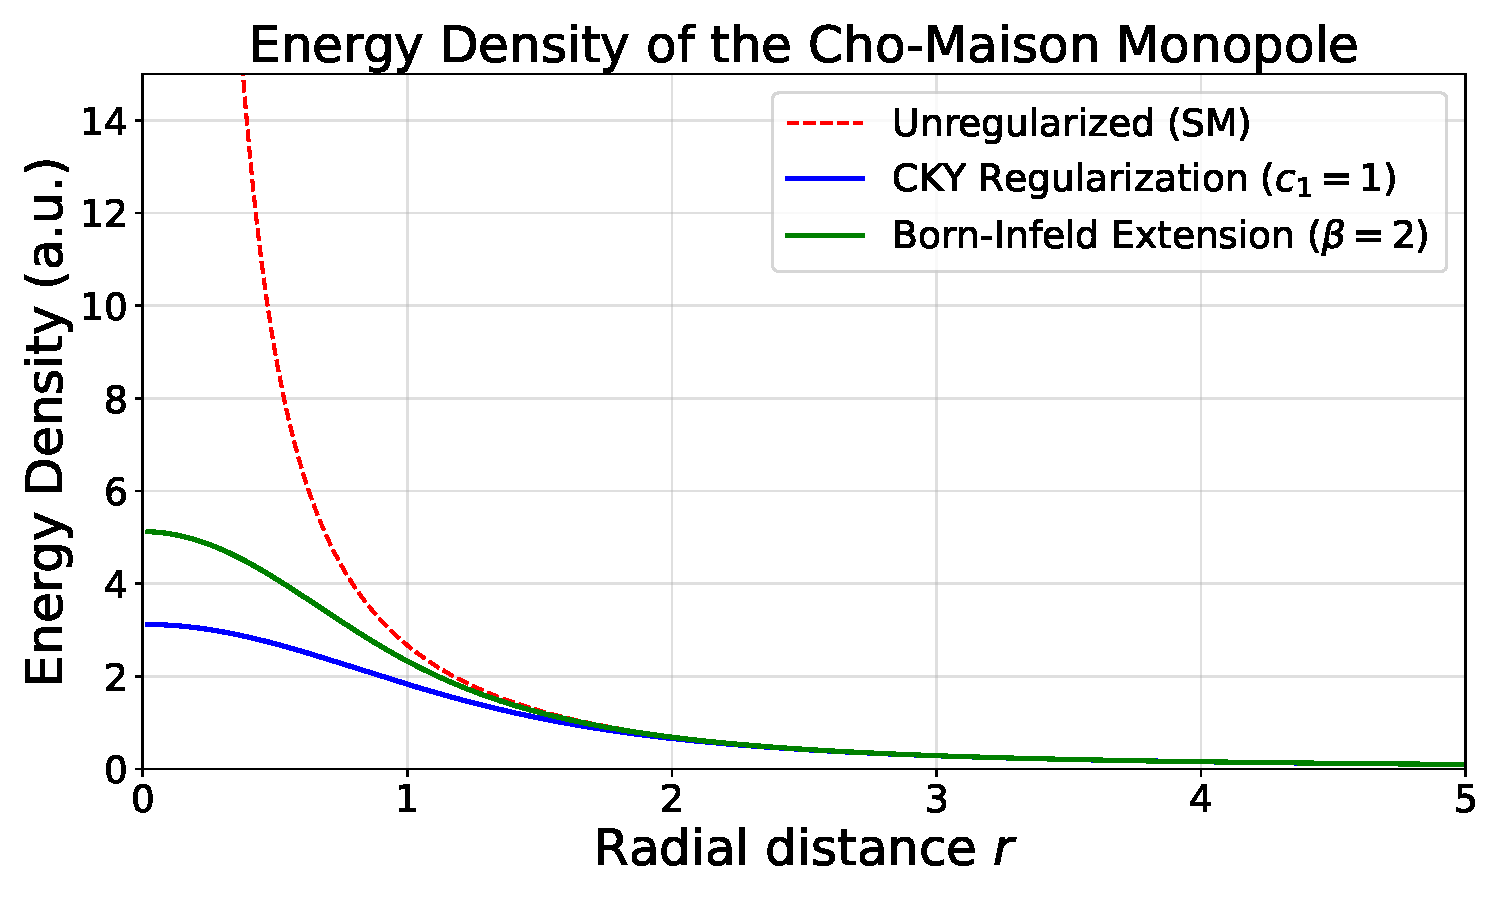
\includegraphics[scale=0.5]{CM_regularization.pdf}
    \caption{Radial profiles of the energy density for the CM monopole under different theoretical frameworks. The dashed curve represents the divergent SM solution. The solid curves demonstrate the taming of this singularity via the CKY regularization scheme (evaluated at $c_1=1$) and the Born-Infeld extension ($\beta=2$). Both regularization schemes successfully yield a finite energy density at $r=0$, allowing for a well-defined monopole mass}
    \label{CMreg}
\end{figure}
\subsection{Some comments about monopoles in Grand Unified Theories}
As we have seen with the 't Hooft-Polyakov solution, magnetic monopoles emerge naturally as finite-energy classical solutions when a non-abelian gauge group is spontaneously broken into a $U(1)$ subgroup. Since the Standard Model is hypothesized to be embedded into a larger  Grand Unified Theory (GUT) gauge group \cite{GeorgiGlashow1974} (such as $SU(5)$ or $SO(10)$) this inherently requires the existence of GUT monopoles.

The mass of these GUT monopoles can be estimated following the same principles as the previous models. The monopole mass is roughly $M \sim m_{V}/\tilde{g}^{2}$, where $m_{V}$ corresponds to the mass of the superheavy vector gauge bosons responsible for the GUT symmetry breaking. For typical unification scales, this leads to an enormous predicted mass in the range of $\mathcal{O}(10^{14}-10^{16})$ GeV. Consequently, such monopoles are far too massive to be pair-produced at the LHC or any foreseeable accelerator. The only physical possibility to observe them relies on direct cosmic searches, although we must bear in mind that their primordial density is expected to be severely diluted due to the exponential expansion during cosmic inflation \cite{Guth1981}.

However, we must remark that the existence of monopoles in GUTs only strictly requires that the $U(1)$ of electromagnetism is embedded in a compact larger group. Therefore, alternative symmetry-breaking patterns might lead to significantly lighter monopoles. For instance, the breaking of an initial $SO(10)$ group down to the Standard Model via an intermediate cross-product group like $SU(4) \times SU(2) \times SU(2)$ could yield intermediate-mass monopoles, depending on the lower energy scale of the secondary symmetry breaking \cite{Lazarides1980}.

Finally, a striking phenomenological feature of GUT monopoles is the Callan-Rubakov effect. Because of the nontrivial gauge boson structure in the core of a GUT monopole, baryon-number-violating processes are unsuppressed. This implies that a traversing GUT monopole can act as a catalyst for nucleon decay (for instance, prompting proton decay into a positron and a neutral pion, $p \rightarrow e^{+} + \pi^{0}$) \cite{Rubakov1981}. This catalytic effect provides a unique indirect signature that is heavily exploited in modern astrophysical detectors and neutrino telescopes.
\section{Dyons}
\subsection{Schwinger dyons}
As pointed out by Julian Schwinger \cite{doi:10.1126/science.165.3895.757}, the DQC can be understood as a particular case derived from the continuous symmetries of Maxwell's equations, specifically arising from the $e \leftrightarrow g$ duality. In CGS units, the generalized Maxwell's equations in the presence of magnetic sources are:
$$\nabla \cdot \boldsymbol{E} = 4\pi\rho_e \quad ; \quad \nabla \cdot \boldsymbol{B} = 4\pi\rho_m \ .$$
$$-\nabla \times \boldsymbol{E} = \frac{1}{c}\partial_t \boldsymbol{B} +\frac{4\pi}{c} \boldsymbol{j}_m \quad ; \quad \nabla \times \boldsymbol{B} =\frac{1}{c} \partial_t \boldsymbol{E}+ \frac{4\pi}{c} \boldsymbol{j}_e\ . $$
These equations exhibit a clear discrete symmetry:
\begin{equation}
    \boldsymbol{E} \mapsto \boldsymbol{B} \; ; \; \boldsymbol{B} \mapsto -\boldsymbol{E} \; , \; \rho_e \mapsto \rho_m \; ; \; \rho_m \mapsto -\rho_e\ ,
\end{equation}
where the currents $\boldsymbol{j}_m$ and $\boldsymbol{j}_e$ transform identically to their respective charge densities. This duality seamlessly accommodates the dynamics of a point particle carrying both electric and magnetic charges, the so-called \textit{dyon} (Schatten, 1970).Furthermore, this discrete transformation is merely a special case of a continuous $SO(2)$ symmetry that rotates the fields and their sources:
\begin{equation}
    \begin{pmatrix} \boldsymbol{E}' \\ \boldsymbol{B}' \end{pmatrix} = \begin{pmatrix} \cos\theta & \sin\theta \\ -\sin\theta & \cos\theta \end{pmatrix} \begin{pmatrix} \boldsymbol{E} \\ \boldsymbol{B} \end{pmatrix} \; ; \; \begin{pmatrix} \rho_e' \\ \rho_m' \end{pmatrix} = \begin{pmatrix} \cos\theta & \sin\theta \\ -\sin\theta & \cos\theta \end{pmatrix} \begin{pmatrix} \rho_e \\ \rho_m \end{pmatrix}\ .
\end{equation}
This continuous symmetry provides a simple mechanism to explain the empirical absence of magnetic charges. If the ratio of magnetic to electric charge in all matter is a universal constant, such that $\rho_m / \rho_e = \tan\theta$ (or $g/e = \tan\theta$), a global rotation by $-\theta$ completely eliminates all magnetic sources from the theory, reducing it back to standard electrodynamics. Conversely, these rotations also define invariant quantities for any two dyons with charges $(e_1, g_1)$ and $(e_2, g_2)$. For instance, the bilinear form $e_1 e_2 + g_1 g_2$ is strictly invariant:
\begin{equation}
    e_1' e_2' + g_1' g_2' = e_1 e_2 (\cos^2\theta + \sin^2\theta) + g_1 g_2 (\sin^2\theta + \cos^2\theta) = e_1 e_2 + g_1 g_2\ .
\end{equation}
Similarly, the cross term $e_1 g_2 - e_2 g_1$ is conserved under this $SO(2)$ rotation:
\begin{equation}
    e_1' g_2' - e_2' g_1' = e_1 g_2 (\cos^2\theta + \sin^2\theta) - e_2 g_1 (\cos^2\theta + \sin^2\theta) = e_1 g_2 - e_2 g_1\ .
\end{equation}

Let us now examine the dynamics of a non-relativistic dyon of mass $m$ and charges $(e_1, g_1)$ moving with velocity $\boldsymbol{v}$ in the presence of a static dyon $(e_2, g_2)$ located at the origin. The Newton equation reads:
\begin{align}
    \begin{split}
         m \frac{d\boldsymbol{v}}{dt} &= e_1 (\boldsymbol{E} + \frac{1}{c}\boldsymbol{v} \times \boldsymbol{B}) + g_1 (\boldsymbol{B} - \frac{1}{c}\boldsymbol{v} \times \boldsymbol{E})\\
         &= (e_1 e_2 + g_1 g_2) \frac{\boldsymbol{r}}{r^3} + (e_1 g_2 - e_2 g_1) \boldsymbol{v} \times \frac{\boldsymbol{r}}{r^3}\ .
    \end{split}
\end{align}
To identify the total angular momentum, we take the cross product with $\boldsymbol{r}$:
\begin{align}
    \begin{split}
  \boldsymbol{r} \times \left( m \frac{d\boldsymbol{v}}{dt} \right) &= (e_1 g_2 - e_2 g_1) \frac{1}{c}\frac{\boldsymbol{r} \times (\boldsymbol{v} \times \boldsymbol{r})}{r^3}\\
  &=(e_1 g_2 - e_2 g_1) \frac{1}{c}\left( \frac{\boldsymbol{v} r - \boldsymbol{r}\dot{r}}{r^2} \right)=(e_1 g_2 - e_2 g_1) \frac{1}{c}\frac{d}{dt}\left( \frac{\boldsymbol{r}}{r} \right)\ .
    \end{split}
\end{align}
Applying the vector triple product identity $\boldsymbol{r} \times (\boldsymbol{v} \times \boldsymbol{r}) = r^2 \boldsymbol{v} - \boldsymbol{r}(\boldsymbol{r} \cdot \boldsymbol{v})$, and noting that $\boldsymbol{v} = \dot{\boldsymbol{r}}$, we find:
\begin{equation}
    \boldsymbol{J} \equiv \boldsymbol{L} - (e_1 g_2 - e_2 g_1)\frac{1}{c} \hat{\boldsymbol{r}} \quad \text{such that} \quad \frac{d\boldsymbol{J}}{dt} = 0\ .
\end{equation}
Note that the second term is the field contribution to the angular momentum, as expected. Now, following the Bohr-Sommerfeld quantization condition, the component of the angular momentum stored in the electromagnetic field must be quantized in half-integer units of $\hbar$. Thus, we arrive at the generalized quantization condition:
\begin{equation}
    (e_1 g_2 - e_2 g_1) \frac{1}{\hbar c} = \frac{n}{2} \; , \quad n \in \mathbb{Z}\ .
\end{equation}
However, Schwinger argued that $n$ must be restricted exclusively to even integers ($n = 2k$) to remain consistent with the absence of observable magnetic charges in matter. His reasoning is rooted in the algebra of quantum angular momentum. If ordinary matter is magnetically neutral, then there exists a purely magnetic counterpart at some position $\boldsymbol{R}$ to neutralize the system. The electromagnetic angular momentum would then acquire a new term:
\begin{equation}
    \boldsymbol{J}_{\text{new.}}^{\text{EM}} = -\frac{eg}{c} \left\{ \frac{\boldsymbol{r}}{r} - \frac{\boldsymbol{r}-\boldsymbol{R}}{|\boldsymbol{r}-\boldsymbol{R}|} \right\}\ .
\end{equation}
In the limit as $\boldsymbol{R} \to 0$, this term vanishes, leaving the angular momentum of the system completely orbital. Because purely orbital angular momentum must possess integer eigenvalues, and integer quantum eigenvalues cannot be continuously deformed into half-integers, the original field angular momentum must have also been an integer. Consequently, $n = 2k$.

As a final check, if we evaluate the specific case of an ordinary electron interacting with a pure Schwinger monopole, we set $(e_1, g_1) = (e, 0)$ and $(e_2, g_2) = (0, g)$. Applying Schwinger's even-integer rule ($n = 2k$), the generalized relation simplifies to:
\begin{equation}
    \frac{eg}{\hbar c} = 2n \; , \quad n \in \mathbb{N}\ ,
\end{equation}
as expected.


\subsection{Julia-Zee dyons}
Dyons emerge as classical solutions within the 't HP model by relaxing the temporal gauge condition. Specifically, the temporal gauge field is generalized to:
\begin{equation}
    A_0^a=\frac{x^a}{r^2}J(r)\ .
\end{equation}
Consequently, we must introduce the respective kinetic terms, $(D_{0}\phi^{a})^{2}$ and $(F_{0i}^{a})^{2}$, into the energy functional. Note, however, that $(D_{0}\phi^{a})^{2}$ identically vanishes because the scalar field $\phi^{a}$ is time-independent and aligned parallel to $A_{0}^{a}$. On the other hand, similar arguments for the field strength tensor yield:
\begin{equation}
    F_{0i}^a=-D_i A_0^a\ .
\end{equation}
In this context, the scalar field $\phi^{a}$ and the temporal gauge component $A_{0}^{a}$ play analogous roles. The modified Julia-Zee energy functional can thus be expressed as an extension of the original HP functional:
\begin{equation}
    E_{\text{JZ}}\equiv E_{\text{HP}}+\int_{\mathbb R^3} d^3 \boldsymbol{x}\ \frac{1}{2}(D_iA^a_0)^2\ ,
\end{equation} 
among the resulting modifications to the field equations, of special interest is the condition arising from the variation with respect to $J(r)$, namely $\delta_{J}E=0$. This yields the following differential equation:
\begin{equation}\label{edo}
    r^2 J''(r)=2J(r)f^2(r)\ .
\end{equation}
Since the $U(1)_{\text{EM}}$ field strength tensor remains unmodified, the magnetic field for the monopole is preserved. Additionally, a novel electric field emerges through the relation:
\begin{equation}
    \mathcal E_i=\hat{\phi}^a F^a_{0i}=\frac{-x^i}{r}\frac{d}{dr}\left(\frac{J(r)}{\tilde g r} \right)\ .
\end{equation}
Consequently, the associated electric charge $q$ is obtained by computing the electric flux at spatial infinity:
\begin{equation}
q\equiv \oint_{\mathbb S^2_\infty}d^2 \boldsymbol x\ n^i \mathcal E_i=4\pi \lim_{r\to \infty}\left[-r^2 \frac{d}{dr}\left(\frac{J(r)}{\tilde g r} \right) \right]\ .
\end{equation}
Since $f(r) \to 0$ as $r \to \infty$, the asymptotic solution to the differential equation for $J(r)$ is $J(r) = C_{1}r + C_{2}$. Substituting this into the charge integral yields:
\begin{equation}
    q= \frac{4\pi \hbar c}{\tilde g^2}\tilde g C_2(v)\ .
\end{equation}
This non-vanishing electric charge confirms the existence of the dyon solution \cite{julia1975}.

To estimate the mass of this dyon, we can determine a theoretical lower bound by analyzing the BPS limit. By introducing a weak mixing angle $\theta$, the energy functional can be rewritten as:
\begin{equation}
    E=\int_{\mathbb R^3}d^3 \boldsymbol x\left[\frac{1}{2}(B_i^a-D_i\phi^a\cos\theta)^2+\frac{1}{2}(E_i^a-D_i\phi^a\sin\theta)^2+\cos\theta B_i^a D_i\phi^a+\sin\theta E_i^aD_i\phi^a \right]\ .
\end{equation}
Imposing $\delta E(\theta) = 0$ for a fixed mixing angle yields the minimum energy configuration:
\begin{equation}
    E_{\text{min}}(\theta)=v(g\cos\theta+q\sin\theta)\ .
\end{equation}
Finally, minimizing this energy with respect to the mixing angle $\theta$ retrieves the Schwinger dyon relation, $\tan\theta = q/g$, which establishes the fundamental lower mass bound for the dyon:
\begin{equation}
    M=v\sqrt{g^2+q^2}\ .
\end{equation}
\subsection{The Witten effect}

TBD

\section{Monopole phenomenology}
\subsection{Classical scattering of two dyons}
Let us consider the classical scattering of two dyons with charges $(e_1, g_1)$ and $(e_2, g_2)$. Recall from our previous analysis of $SO(2)$ duality rotations that the following combined charges are strictly invariant:
\begin{equation}
    q = e_1 e_2 + g_1 g_2 \quad \text{and} \quad \kappa = e_1 g_2 - e_2 g_1\ .
\end{equation}
In the center-of-mass frame, where $\mu = (m_1^{-1} + m_2^{-1})^{-1}$ is the reduced mass, $\boldsymbol{r}$ is the relative position vector, and $\boldsymbol{v} = \dot{\boldsymbol{r}}$ is the relative velocity, the spherical symmetry of the interaction guarantees the conservation of both the total energy $E$ and the total angular momentum $\boldsymbol{J}$:
\begin{equation}
    E = \frac{1}{2}\mu v^2 + \frac{q}{r} \quad ; \quad \boldsymbol{J} = \boldsymbol{\ell} + \kappa\hat{\boldsymbol r} \quad (\boldsymbol{\ell} \equiv \boldsymbol{r} \times \mu\boldsymbol{v})\ .
\end{equation}
Because the purely orbital angular momentum $\boldsymbol{\ell}$ is strictly perpendicular to the position vector $\boldsymbol{r}$, the total angular momentum $\boldsymbol{J}$ traces out a cone around the trajectory \cite{Birkeland1896, Poincare1896}, as depicted in Figure \ref{cone}. We can parameterize this geometry by introducing a scattering angle $\chi$. Setting $\ell = |\boldsymbol{\ell}|$, the geometry of the cone dictates that:
\begin{equation}
    \cot(\chi/2) = \frac{\ell}{|\kappa|} \quad \text{and} \quad \sin\alpha = \cos(\chi/2)\ .
\end{equation}
Now, denoting as $(r, \alpha, \varphi)$ the spherical coordinates induced from the previous diagram, we observe that under a $\Delta\varphi$ rotation ($\Delta r = \Delta\alpha = 0$), the following quantity remains constant:
\begin{equation}
    \cos(\chi/2)\Delta\varphi = \sin\alpha\,\Delta\varphi\ . 
\end{equation}
In particular, we will define $\Delta\tilde{\varphi} \equiv \varphi_{\text{out}} - \varphi_{\text{in}}$, as the difference between the azimuthal angles in $\hat{\boldsymbol r}_{\text{out}}$ (at $t \to \infty$) and $-\hat{\boldsymbol r}_{\text{in}}$ (at $t \to -\infty$), as well as the angle $\chi$ through:
\begin{equation}
    \cos(\chi/2)\Delta\tilde{\varphi}/2 = \xi/2\ .
\end{equation}
It is also convenient to define the angle given by the projection of these two:
\begin{equation}
    \hat{\boldsymbol r}_{\text{in}} \cdot \hat{\boldsymbol r}_{\text{out}} \equiv \cos(\pi - \Theta)\ .
\end{equation}
Then, the new angle $\Theta$ can be expressed in terms of $\xi, \chi$ as:
\begin{equation}
    \cos\left(\frac{\Theta}{2}\right) = \cos(\chi/2)\left|\sin\left(\frac{\xi/2}{\cos(\chi/2)}\right)\right|\ .
\end{equation}
\begin{figure}[ht!]
    \centering 
    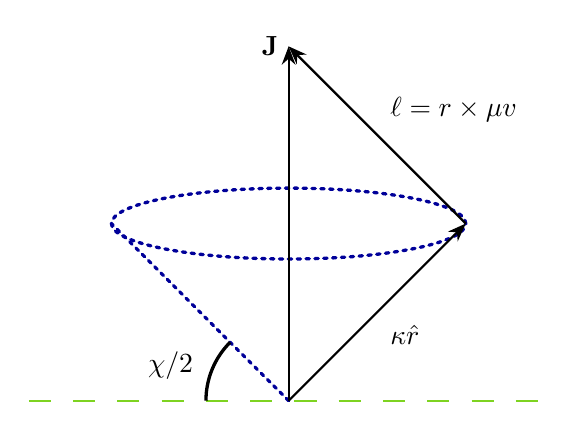
\begin{tikzpicture}[>=Stealth, scale=1.5]

    % Horizontal dashed line (green)
    \draw[color={rgb, 255:red, 126; green, 211; blue, 33 }, thick, dash pattern=on 8pt off 8pt] (-2.2,0) -- (2.2,0);

    % Dotted lines for the cone (blue)
    \draw[blue!60!black, very thick, dotted, line cap=round] (0,1.5) ellipse (1.5 and 0.3);
    \draw[blue!60!black, very thick, dotted, line cap=round] (0,0) -- (-1.5,1.5);

    % Vertical vector J
    \draw[->, thick] (0,0) -- (0,3) node[left] {$\mathbf{J}$};

    % Vector \kappa \hat{r}
    \draw[->, thick] (0,0) -- (1.5,1.5) node[midway, below right=1pt] {$\kappa\hat{\boldsymbol{r}}$};

    % Vector \ell
    \draw[->, thick] (1.5,1.5) -- (0,3) node[midway, above right=1pt] {$\ell = \boldsymbol{r} \times \mu\boldsymbol{v}$};

 % Corrected Angle arc for \chi/2 (from horizontal to the dotted line)
    \draw[very thick] (-0.7,0) arc (180:135:0.7);
    \node at (-1.0, 0.3) {$\chi/2$};

\end{tikzpicture}
\caption{Picture showcasing the confination of the relative motion within a cone in the direction of the angular momentum.}
\label{cone}
\end{figure}

There are several subtleties hidden beneath these computations. Firstly, the angle $\xi$ depends whether on the potential is repulsive ($q > 0$) or attractive ($q < 0$) in a non-continuous way. To see this, it is sufficient to focus on the energy:
\begin{equation}
    E = \frac{\mu}{2}(\dot{r}^2 + r^2\sin^2\alpha\,\dot{\varphi}^2) + \frac{q}{r}= \frac{\mu}{2}(\dot{r}^2 + r^2\dot{\varphi}^2\cos^2(\chi/2)) + \frac{q}{r} = \frac{\mu v_0^2}{2}\ ,
\end{equation}

with $v_0$ denoting the velocity of the incoming dyon, which defines the impact parameter $b$ through $l = \mu v_0 b$. Using the standard substitution $u = r^{-1}$, and denotinf $\psi\equiv \varphi \cos(\chi/2)$, the energy conservation equation transforms into the orbit equation:
\begin{equation}
    \frac{d^2 u}{d\psi^2} + u = -\frac{\mu q}{\ell^2}\ .
\end{equation}
Choosing the angle $\psi_0$ to correspond to the periapsis, the general solution takes the form:
\begin{equation}
    u(\psi) = A\cos(\psi - \psi_0) - \frac{q\mu}{\ell^2}\ .
\end{equation}
Evaluating this solution at the asymptotic limit where $u \to 0$ ($r \to \infty$) yields the amplitude $A = \frac{\mu}{\ell^2}\sqrt{v_0^2 \ell^2 + q^2}$ and establishes the relation for the scattering angle $\xi/2$:
\begin{equation}
    \tan(\xi/2) = \frac{v_0 \ell}{q}= \frac{|\kappa| v_0}{q} \cot(\chi/2)\ .
\end{equation}
Notice that the sign of $q$ constrains the sign of $\cos(\xi/2)$ and thus, limits the range of the angle $\xi$. If $q > 0$, then the tangent can be inverted straightforwardly, while the repulsive case picks up a $\pi$ term:
\begin{equation}
    \xi/2 = \begin{cases} \arctan\left(\frac{|\kappa|v_0}{q} \cot(\chi/2)\right), & q > 0\ , \\ \pi - \arctan\left(\frac{|\kappa|v_0}{|q|} \cot(\chi/2)\right), & q < 0 \ . \end{cases}
\end{equation}
Furthermore, projecting the incoming and outgoing asymptotic directions defines the physical scattering angle $\Theta$, where $\hat{\boldsymbol{r}}_{in} \cdot \hat{\boldsymbol{r}}_{out} = \cos(\pi - \Theta)$. The relationship between the impact parameter and $\Theta$ is notably multi-valued, reflecting the fact that dyons can wrap around each other multiple times before escaping. This yields a discrete set of impact parameters $b_n$ for a given observation angle $\Theta$. Indeed, in the particular case $\xi=\Theta=0$:
\begin{equation}
    \sin\left(\frac{\pi}{2\cos(\chi/2)}\right) = 0 \iff \cos\left(\frac{\chi_n}{2}\right) = \frac{1}{2n} \; , \quad n \in \mathbb{N}\ .
\end{equation}
Hence:
\begin{equation}
    b_n = \frac{|\kappa|}{\mu v_0}\frac{1}{\sqrt{4n^2 - 1}} \; , \quad n \in \mathbb{N}\ ,
\end{equation}
for a fixed $\Theta$. This is a crucial result since in a classical 2-body scattering scenario, the differential cross-section is directly related
to the impact parameter via:
\begin{equation}
    \frac{d\sigma}{d\Omega} = \left|\frac{b\,db}{\sin\Theta\,d\Theta}\right| = \sum_{n \in \mathbb{N}} \left|\frac{b_n db_n}{\sin\Theta\,d\Theta}\right|\ ,
\end{equation}
the consequent derivatives are trivial and yield the general expression:
\begin{equation}
    \frac{d\sigma}{d\Omega} = \left(\frac{\kappa}{\mu v_0}\right)^2 \sum_{n \in \mathbb{N}} \frac{1}{4\sin^4(\chi/2)} \left|\frac{\sin\chi_n\,d\chi_n}{\sin\Theta\,d\Theta}\right|\ ,
\end{equation}
whose divergences are located at $\Theta = \pi$ for $\chi_n \neq 0$ and at $d\Theta/d\chi_n$, both to be evaluated numerically.Of special interest is the $\Theta \ll 1$ (or $b \to \infty$) case, where the branches collapse into a unique branch with $\chi \to 0$, modifying the angle $\xi$ to follow:
\begin{equation}
    \xi/2 = \frac{\pi}{2} - \frac{q\chi}{2|\kappa|v_0} + \mathcal{O}(\chi^2)\ ,
\end{equation}
and the angle $\Theta$ to:
\begin{equation}
    \Theta = \chi\sqrt{1 + q^2 / \kappa^2 v_0^2} + \mathcal{O}(\chi^2)\ .
\end{equation}
Consequently, the differential cross-section within this limit reads \cite{Milton2006}:
\begin{equation}
    \frac{d\sigma}{d\Omega} \approx \left(\frac{1}{2\mu v_0}\right)^2 \left\{ \left(\frac{e_1 e_2 + g_1 g_2}{v_0}\right)^2 + \left(\frac{e_1 g_2 - g_1 e_2}{c}\right)^2 \right\} \frac{1}{(\Theta/2)^4}\ ,
\end{equation}
note CGS units were recovered. The plot of this formula is depicted in Figure \ref{rutherford}, showcasing the multi-valued nature of the angle $\Theta$. If we consider the purely electromagnetic scattering of an electron $(e, 0)$ off a magnetic monopole $(0, g)$, this formula recovers the exact functional form of standard Rutherford scattering via the dual mapping:
\begin{equation}\label{gbeta}
    \frac{e^2}{v_0} \mapsto \frac{eg}{c}\ .
\end{equation}
This direct equivalence between velocity and magnetic coupling is frequently used in perturbative monopole model-building, as we will see in the next sections.
\begin{figure}[ht!]
    \centering
    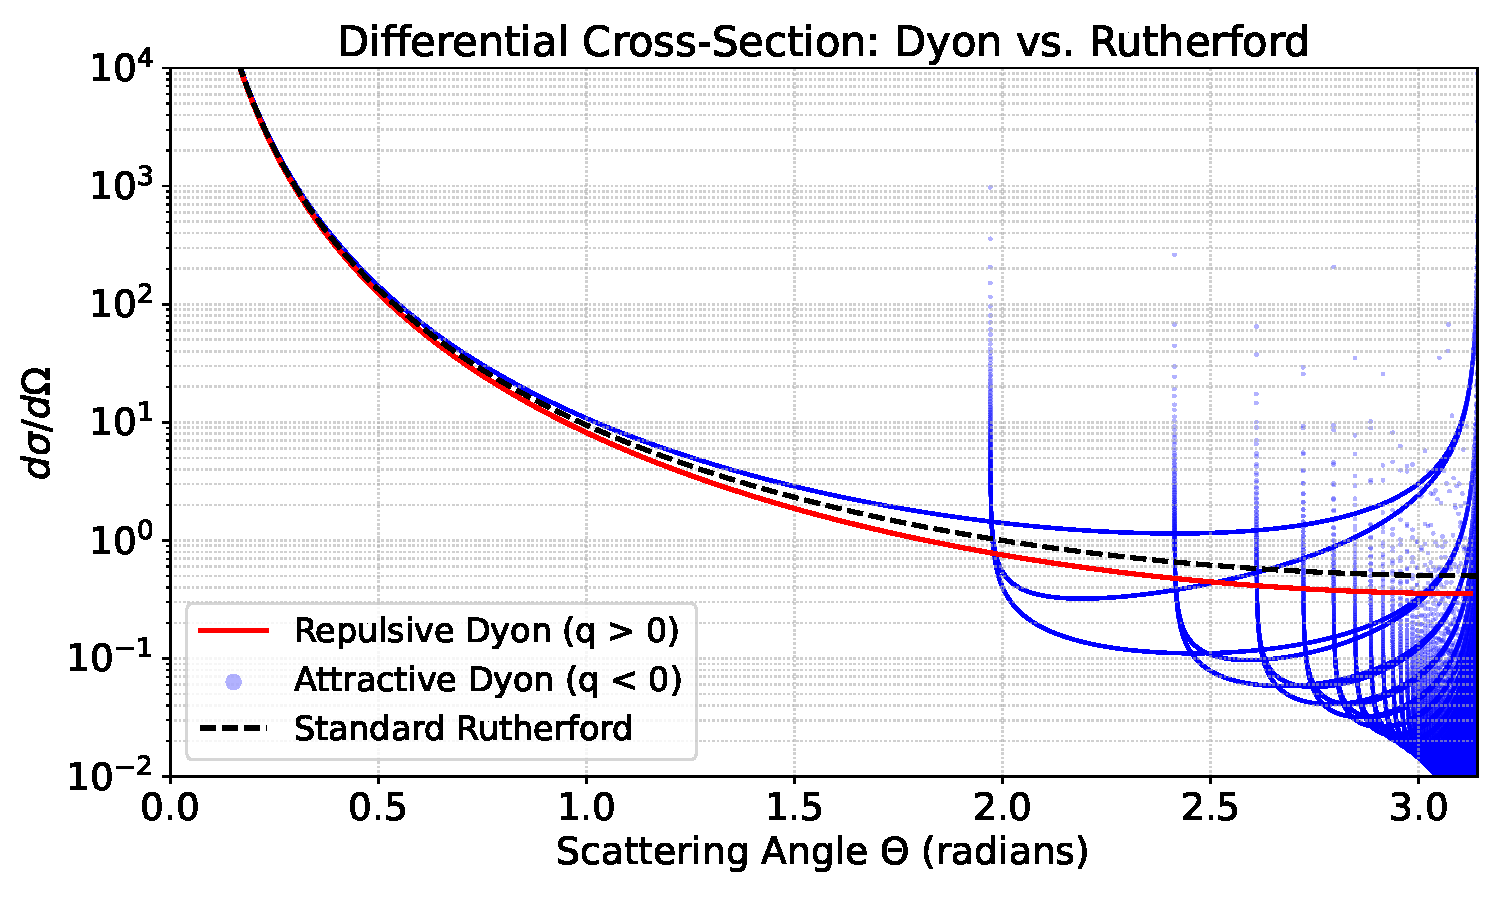
\includegraphics[scale=0.5]{rutherford.pdf}
    \caption{Differential cross-section $d\sigma/d\Omega$ as a function of the scattering angle $\Theta$ for the classical scattering of two dyons. The solid curves denote the exact cross-sections for repulsive ($q > 0$) and attractive ($q < 0$) interactions. The dashed line represents the standard Rutherford scattering profile.}
    \label{rutherford}
\end{figure}
\subsection{To be continued, dual theories yadayada}

\section{Detection techniques}
\textbf{Remark}: For this section, \cite{2016,mitsou2026magneticmonopolesdirac} and references therein were used.

It is a well-established principle in classical electrodynamics that charged particles deposit a fraction of their energy as they traverse matter. By virtue of electric-magnetic duality, magnetic monopoles are expected to undergo an analogous energy-loss process when interacting with a medium.
\subsection{Ionization and excitation}\label{51}
The dynamics of a monopole-matter interaction are primarily governed by the monopole's velocity, denoted by $\beta$, and the intrinsic properties of the medium. Based on $\beta$, the energy-loss mechanisms can be classified into three dominant scenarios:
 \begin{itemize}
    \item \textbf{Ionization:} this is the dominant energy-loss mechanism for fast monopoles, which are defined via the bound $\beta> 0.05$. This mechanism leads to the production of free electrons.
    \item \textbf{Atomic excitation:} instead of producing free electrons, the energy of the monopole induces atomic transitions to higher energy states. It is the main mechanism for slow monopoles within the bounds $10^{-3}\le \beta \le 10^{-2}$.
    \item \textbf{Elastic collisions with atoms:} In this ultra-slow regime ($\beta<10^{-3}$), the kinetic energy transferred is insufficient to induce atomic transitions. Instead, the interaction proceeds via elastic recoil generated by the coupling between the monopole and the magnetic moments of the target nuclei. Consequently, the energy loss is heavily dependent on whether the medium is diamagnetic or paramagnetic.
 \end{itemize}
 
It is worth noting that all these mechanisms generally describe non-relativistic to moderately relativistic magnetic monopoles. Because of this characteristically non-relativistic behavior, the ionization energy loss per unit path length (namely, $-dE/dx$) for a standard particle with electric charge $z$ is given by a modified classical Bethe-Bloch formula:
 \begin{equation}\label{bethebloch}
    -\frac{dE}{dx}=K\frac{Z}{A}\frac{z^2}{\beta^2}\left[\frac{1}{2}\log\left(\frac{2m_e \beta^2\gamma^2 T_{\text{max.}}}{I^2} \right)-\beta^2-\frac{\delta(\beta \gamma)}{2} \right]\ .
 \end{equation} 
Here, $K = 4\pi N_A r_e^2 m_e$ (where $m_e$ and $r_e$ are the electron mass and classical radius, respectively, and $N_A$ is the Avogadro number), $\gamma$ is the Lorentz factor, and $Z$, $A$, and $I$ represent the atomic number, mass number, and mean excitation energy of the medium, respectively. $T_{\text{max}}$ denotes the maximum kinetic energy transferred to a free electron during a single collision. The density effect correction, $\delta(\beta\gamma)$, is introduced to tame the unphysical logarithmic divergence that appears in the ultra-relativistic limit ($\beta \rightarrow 1$) due to medium polarization fields. Consequently, $\delta(\beta\gamma)$ yields a significant contribution in solids and liquids, but remains negligible for gases.

To adapt this framework for a magnetic monopole carrying a charge $g = n g_D$, the Bethe-Bloch formula must be modified to:
\begin{equation}\label{betheblochmm}
    -\frac{dE}{dx}=K\frac{Z}{A}g^2\left[\log\left(\frac{2m_e\beta^2\gamma^2}{I} \right)+\frac{K(g)}{2}-\frac{1}{2}-B(g)-\frac{\delta(\beta\gamma)}{2} \right]\ .
\end{equation}
In this expression, $K(g)$ is the Kazama-Yang-Goldhaber correction, which accounts for the interaction with the tiny intrinsic magnetic moments of the atomic electrons, while $B(g)$ is the Bloch correction, derived from a strictly quantum mechanical treatment of the scattering process. A striking feature of the magnetic stopping power is the absence of the $1/\beta^2$ kinematic factor. Physically, this means that magnetic monopoles lose energy at a slower relative pace. This arises from the compensation provided by the dual substitution mapping $e \mapsto g\beta$ (as established in eq. (\ref{gbeta})).

Furthermore, due to the immense disparity between the fine-structure constants for electric and magnetic charges this is,the ratio $(g_D/e)^2 \approx 68.5^2$, a relativistic magnetic monopole with charge $g_D$ deposits approximately $4700$ times more energy into a medium than an electric charge e traversing the same path. This energy deposition classifies magnetic monopoles as \textit{Highly-Ionizing Particles} (HIPs). Finally, it must be noted that this modified formula is strictly valid only for $\beta$ > 0.1, requiring appropriate extrapolations for slower regimes, as depicted in Figure \ref{betadistributions}.
\begin{figure}[ht!]
    \centering
    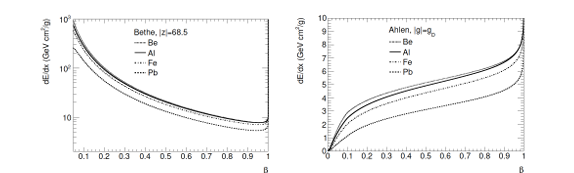
\includegraphics{beta distributions.png}
    \caption{Ionization energy loss $dE/dx$ in various materials as a function of velocity $\beta$ for HIPs possessing an electric charge of $68.5e$ (left) and magnetic charge of $1g_D$ (right). Refine}
    \label{betadistributions} 
\end{figure}
\subsubsection{Scintillators, gaseous detectors and nuclear track detectors }
Because magnetic monopoles leave heavily ionized or excited tracks, their passage through matter can be detected using techniques standardly applied to HIPs. These include scintillators, gaseous detectors, and nuclear track detectors. However, the primary experimental challenge lies in successfully distinguishing a magnetic monopole from other hypothetical or known HIPs.
\begin{itemize}
    \item \textbf{Scintillators}: These detectors rely on the light emission produced during the aforementioned atomic excitation, which occurs within the bounds of $10^{-3}\le \beta \le 10^{-2}$. Contemporary experimental constraints limit the sensitivity of this technique to a minimum velocity of $10^{-3}$.
    \item \textbf{Gaseous detectors}: By exploiting the specific properties of certain gas media (such as hydrogen or helium), these detectors can discern between magnetic monopoles and other ionizing particles, like muons.
    \item \textbf{Nuclear track detectors}: When passing through a nuclear track detector, magnetic monopoles and other HIPs damage the polymer structure, leaving a cylindrical (or cone-shaped) track. The distinct geometry of this cone-shaped trace, combined with the specific $\beta$ distributions (as seen in Figure \ref{betadistributions}), allows to distinguish between electric and magnetic charges.
\end{itemize}

\subsection{Induction}

The induction technique for detecting magnetic monopoles relies on the fact that if the modified Gauss's law for magnetism, $\nabla \cdot \mathbf{B} = 4\pi g$, holds true, a passing magnetic charge will induce a persistent electric current $\Delta i$ in a detection coil. For a coil with $N$ turns and self-inductance $L$, this induced current is given by:
\begin{equation}
    \Delta i=4\pi g \frac{N}{L}\ .
\end{equation}
To measure such a minuscule magnetic flux, the coil must be inductively coupled to a Superconducting Quantum Interference Device (SQUID). In natural units, the elementary flux quantum of the SQUID is $\Phi_0 = \pi/e$, where the factor of $2e$ in the denominator arises from the electric charge of the Cooper pairs. By DQC ($eg_D = 1/2$), the flux emanating from a single fundamental magnetic monopole is exactly $4\pi g_D = 2\pi/e$. Therefore, a single Dirac monopole delivers precisely two superconducting flux quanta ($2\Phi_0$) to the sensing loop. A schematic drawing of the setup is the following:
\begin{figure}[ht!]
    \centering
    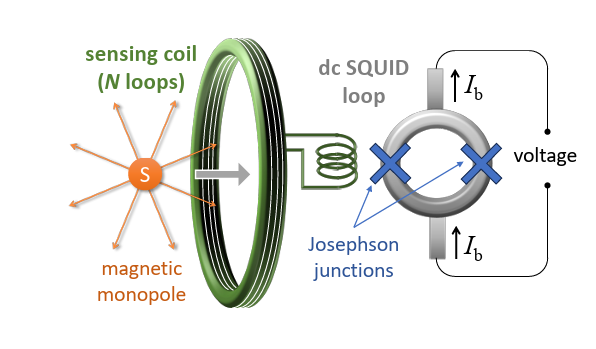
\includegraphics[scale=0.6]{squid.png}
    \caption{Simplified schematic view of a dc SQUID (not to scale). When a MM or a sample passes through the detection coil (green) coupled to a SQUID, a net supercurrent is registered in the SQUID ring.}
    \label{squid}
\end{figure}

When a magnetic monopole (or a macroscopic sample containing a trapped monopole) passes through the detection coil, a net current is registered in the SQUID ring. Because the SQUID is biased with a constant current $I_b$, it effectively operates as a highly sensitive magnetic flux-to-voltage transducer. In the absence of a monopole, a monitor tracking the voltage timeline will display a constant flat line. Conversely, when a magnetic monopole is introduced, a sudden, persistent jump appears on the graph, mathematically behaving like a step function.

The primary experimental challenge associated with these measurements is tied to the extreme sensitivity of the SQUID itself; external disturbances, such as fluctuations in the Earth's magnetic field, can easily alter the readings and create false positives. Nevertheless, induction remains an incredibly powerful method because it allows for fast, continuous, and a virtually infinite number of non-destructive measurements. Because the signal is independent of the monopole's mass or velocity, it stands as one of the most widely used and definitive techniques in contemporary monopole searches.
\section{Search in colliders}
Present and proposed future accelerators feature collisions at a center-of-mass energy, $\sqrt{s}$, of $\mathcal{O}(1-10)$ TeV. Consequently, it is kinematically impossible to search for GUT monopoles. Nevertheless, direct and indirect searches for lighter monopoles have been actively conducted. These efforts involve hadron-hadron, electron-positron, and lepton-hadron collision experiments, utilizing the detection techniques discussed previously. In addition, indirect probes, such as enhanced production rates involving virtual monopoles, are extensively considered.  

\subsection{Monopole production processes}
The direct pair production of magnetic monopoles typically proceeds via three main mechanisms: a Drell-Yan-like (DY) process featuring an s-channel photon, a t-channel photon-fusion diagram, and the strictly non-perturbative Schwinger mechanism. The first two processes (depicted in Figure \ref{Feynmandiag}) rely on perturbation theory. However, the inherently large value of the magnetic fine-structure constant seemingly invalidates a standard perturbative expansion. This theoretical problem can be qualitatively circumvented near the production threshold by introducing a velocity-dependent coupling \cite{Baines2018}:
\begin{equation}\label{runningcoupling}
    e\mapsto g\hat \beta \equiv g \sqrt{1-\frac{4M_{\text{m}}}{s}}\ , 
\end{equation}
While there is no trivial gauge theory that consistently couples a photon to both a fermion and a monopole vertex, diagrammatic approaches remain highly useful. They provide a practical framework to map experimental measurements, such as cross-sections, to indicative physical quantities like the monopole mass.

\begin{figure}[ht!]
    \centering


\tikzset{every picture/.style={line width=0.75pt}} %set default line width to 0.75pt        

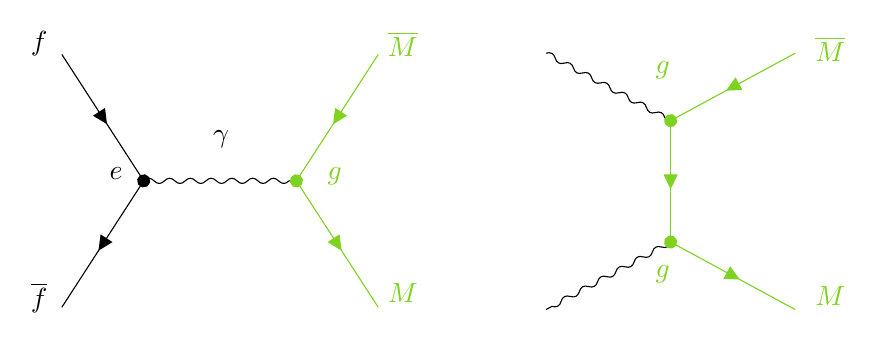
\begin{tikzpicture}[x=0.75pt,y=0.75pt,yscale=-1,xscale=1]
%uncomment if require: \path (0,300); %set diagram left start at 0, and has height of 300

%Straight Lines [id:da3283572493917589] 
\draw    (98.2,69.6) -- (137.63,130.5) ;
\draw [shift={(137.63,130.5)}, rotate = 57.08] [color={rgb, 255:red, 0; green, 0; blue, 0 }  ][fill={rgb, 255:red, 0; green, 0; blue, 0 }  ][line width=0.75]      (0, 0) circle [x radius= 2.68, y radius= 2.68]   ;
\draw [shift={(119.98,103.24)}, rotate = 237.08] [fill={rgb, 255:red, 0; green, 0; blue, 0 }  ][line width=0.08]  [draw opacity=0] (7.14,-3.43) -- (0,0) -- (7.14,3.43) -- cycle    ;
%Straight Lines [id:da3276659901466582] 
\draw    (137.63,130.5) -- (98.2,191.4) ;
\draw [shift={(115.85,164.14)}, rotate = 302.92] [fill={rgb, 255:red, 0; green, 0; blue, 0 }  ][line width=0.08]  [draw opacity=0] (7.14,-3.43) -- (0,0) -- (7.14,3.43) -- cycle    ;
%Straight Lines [id:da054759289151072865] 
\draw    (137.63,130.5) .. controls (139.3,128.83) and (140.96,128.83) .. (142.63,130.5) .. controls (144.3,132.17) and (145.96,132.17) .. (147.63,130.5) .. controls (149.3,128.83) and (150.96,128.83) .. (152.63,130.5) .. controls (154.3,132.17) and (155.96,132.17) .. (157.63,130.5) .. controls (159.3,128.83) and (160.96,128.83) .. (162.63,130.5) .. controls (164.3,132.17) and (165.96,132.17) .. (167.63,130.5) .. controls (169.3,128.83) and (170.96,128.83) .. (172.63,130.5) .. controls (174.3,132.17) and (175.96,132.17) .. (177.63,130.5) .. controls (179.3,128.83) and (180.96,128.83) .. (182.63,130.5) .. controls (184.3,132.17) and (185.96,132.17) .. (187.63,130.5) .. controls (189.3,128.83) and (190.96,128.83) .. (192.63,130.5) .. controls (194.3,132.17) and (195.96,132.17) .. (197.63,130.5) .. controls (199.3,128.83) and (200.96,128.83) .. (202.63,130.5) .. controls (204.3,132.17) and (205.96,132.17) .. (207.63,130.5) -- (211.21,130.5) -- (211.21,130.5) ;
%Straight Lines [id:da43565001470206577] 
\draw [color={rgb, 255:red, 126; green, 211; blue, 33 }  ,draw opacity=1 ]   (250.64,69.6) -- (211.21,130.5) ;
\draw [shift={(211.21,130.5)}, rotate = 122.92] [color={rgb, 255:red, 126; green, 211; blue, 33 }  ,draw opacity=1 ][fill={rgb, 255:red, 126; green, 211; blue, 33 }  ,fill opacity=1 ][line width=0.75]      (0, 0) circle [x radius= 2.68, y radius= 2.68]   ;
\draw [shift={(228.86,103.24)}, rotate = 302.92] [fill={rgb, 255:red, 126; green, 211; blue, 33 }  ,fill opacity=1 ][line width=0.08]  [draw opacity=0] (7.14,-3.43) -- (0,0) -- (7.14,3.43) -- cycle    ;
%Straight Lines [id:da24664349958300247] 
\draw [color={rgb, 255:red, 126; green, 211; blue, 33 }  ,draw opacity=1 ]   (211.21,130.5) -- (250.64,191.4) ;
\draw [shift={(232.99,164.14)}, rotate = 237.08] [fill={rgb, 255:red, 126; green, 211; blue, 33 }  ,fill opacity=1 ][line width=0.08]  [draw opacity=0] (7.14,-3.43) -- (0,0) -- (7.14,3.43) -- cycle    ;
%Straight Lines [id:da8352762541829424] 
\draw    (331.5,69) .. controls (333.76,68.33) and (335.23,69.12) .. (335.9,71.38) .. controls (336.57,73.64) and (338.03,74.43) .. (340.29,73.76) .. controls (342.55,73.09) and (344.02,73.88) .. (344.69,76.14) .. controls (345.36,78.4) and (346.83,79.2) .. (349.09,78.53) .. controls (351.35,77.86) and (352.81,78.65) .. (353.48,80.91) .. controls (354.15,83.17) and (355.62,83.96) .. (357.88,83.29) .. controls (360.14,82.62) and (361.61,83.41) .. (362.28,85.67) .. controls (362.95,87.93) and (364.41,88.72) .. (366.67,88.05) .. controls (368.93,87.38) and (370.4,88.17) .. (371.07,90.43) .. controls (371.74,92.69) and (373.2,93.48) .. (375.46,92.81) .. controls (377.72,92.14) and (379.19,92.94) .. (379.86,95.2) .. controls (380.53,97.46) and (382,98.25) .. (384.26,97.58) .. controls (386.52,96.91) and (387.98,97.7) .. (388.65,99.96) -- (391.5,101.5) -- (391.5,101.5) ;
%Straight Lines [id:da8603175839651677] 
\draw [color={rgb, 255:red, 126; green, 211; blue, 33 }  ,draw opacity=1 ]   (391.5,101.5) -- (391.5,160) ;
\draw [shift={(391.5,134.55)}, rotate = 270] [fill={rgb, 255:red, 126; green, 211; blue, 33 }  ,fill opacity=1 ][line width=0.08]  [draw opacity=0] (7.14,-3.43) -- (0,0) -- (7.14,3.43) -- cycle    ;
%Shape: Boxed Line [id:dp12741350927386197] 
\draw    (391.5,160) .. controls (390.83,162.26) and (389.36,163.05) .. (387.1,162.38) .. controls (384.84,161.71) and (383.38,162.5) .. (382.71,164.76) .. controls (382.04,167.02) and (380.57,167.81) .. (378.31,167.14) .. controls (376.05,166.47) and (374.58,167.27) .. (373.91,169.53) .. controls (373.24,171.79) and (371.78,172.58) .. (369.52,171.91) .. controls (367.26,171.24) and (365.79,172.03) .. (365.12,174.29) .. controls (364.45,176.55) and (362.98,177.34) .. (360.72,176.67) .. controls (358.46,176) and (357,176.79) .. (356.33,179.05) .. controls (355.66,181.31) and (354.19,182.1) .. (351.93,181.43) .. controls (349.67,180.76) and (348.21,181.55) .. (347.54,183.81) .. controls (346.87,186.07) and (345.4,186.87) .. (343.14,186.2) .. controls (340.88,185.53) and (339.41,186.32) .. (338.74,188.58) .. controls (338.07,190.84) and (336.61,191.63) .. (334.35,190.96) -- (331.5,192.5) -- (331.5,192.5) ;
%Straight Lines [id:da09735266193847114] 
\draw [color={rgb, 255:red, 126; green, 211; blue, 33 }  ,draw opacity=1 ]   (451.5,69) -- (391.5,101.5) ;
\draw [shift={(391.5,101.5)}, rotate = 151.56] [color={rgb, 255:red, 126; green, 211; blue, 33 }  ,draw opacity=1 ][fill={rgb, 255:red, 126; green, 211; blue, 33 }  ,fill opacity=1 ][line width=0.75]      (0, 0) circle [x radius= 2.68, y radius= 2.68]   ;
\draw [shift={(418.16,87.06)}, rotate = 331.56] [fill={rgb, 255:red, 126; green, 211; blue, 33 }  ,fill opacity=1 ][line width=0.08]  [draw opacity=0] (7.14,-3.43) -- (0,0) -- (7.14,3.43) -- cycle    ;
%Straight Lines [id:da05591492044881907] 
\draw [color={rgb, 255:red, 126; green, 211; blue, 33 }  ,draw opacity=1 ]   (391.5,160) -- (451.5,192.5) ;
\draw [shift={(424.84,178.06)}, rotate = 208.44] [fill={rgb, 255:red, 126; green, 211; blue, 33 }  ,fill opacity=1 ][line width=0.08]  [draw opacity=0] (7.14,-3.43) -- (0,0) -- (7.14,3.43) -- cycle    ;
\draw [shift={(391.5,160)}, rotate = 28.44] [color={rgb, 255:red, 126; green, 211; blue, 33 }  ,draw opacity=1 ][fill={rgb, 255:red, 126; green, 211; blue, 33 }  ,fill opacity=1 ][line width=0.75]      (0, 0) circle [x radius= 2.68, y radius= 2.68]   ;


% Text Node
\draw (169.84,104.78) node [anchor=north west][inner sep=0.75pt]    {$\gamma $};
% Text Node
\draw (82,178.28) node [anchor=north west][inner sep=0.75pt]    {$\overline{f}$};
% Text Node
\draw (82,56.97) node [anchor=north west][inner sep=0.75pt]    {$f$};
% Text Node
\draw (120,123) node [anchor=north west][inner sep=0.75pt]    {$e$};
% Text Node
\draw (254,178.77) node [anchor=north west][inner sep=0.75pt]  [color={rgb, 255:red, 126; green, 211; blue, 33 }  ,opacity=1 ]  {$M$};
% Text Node
\draw (254,57.48) node [anchor=north west][inner sep=0.75pt]  [color={rgb, 255:red, 126; green, 211; blue, 33 }  ,opacity=1 ]  {$\overline{M}$};
% Text Node
\draw (225,123) node [anchor=north west][inner sep=0.75pt]  [color={rgb, 255:red, 126; green, 211; blue, 33 }  ,opacity=1 ]  {$g$};
% Text Node
\draw (383,72) node [anchor=north west][inner sep=0.75pt]  [color={rgb, 255:red, 126; green, 211; blue, 33 }  ,opacity=1 ]  {$g$};
% Text Node
\draw (383,170) node [anchor=north west][inner sep=0.75pt]  [color={rgb, 255:red, 126; green, 211; blue, 33 }  ,opacity=1 ]  {$g$};
% Text Node
\draw (460,180.4) node [anchor=north west][inner sep=0.75pt]  [color={rgb, 255:red, 126; green, 211; blue, 33 }  ,opacity=1 ]  {$M$};
% Text Node
\draw (460,59.9) node [anchor=north west][inner sep=0.75pt]  [color={rgb, 255:red, 126; green, 211; blue, 33 }  ,opacity=1 ]  {$\overline{M}$};


\end{tikzpicture}
\caption{Drell-Yan production diagram (left) and photon fusion production diagram (right). Fermions can be both quarks or leptons, while the photons may be radiated off from collinding fermions or nuclei.}
\label{Feynmandiag}
\end{figure}
While DY and photon-fusion processes rely on standard perturbative calculations (even though they are problematic) the Schwinger effect offers a strictly non-perturbative mechanism for monopole pair creation. In standard QED, the Schwinger effect describes the spontaneous creation of electron-positron pairs from the vacuum in the presence of an incredibly strong electric field. By virtue of the electric-magnetic duality, an analogous phenomenon must exist for magnetic charges: a sufficiently strong magnetic field can spontaneously produce magnetic monopole-antimonopole pairs from the vacuum. For a magnetic field $\boldsymbol{B}$, the non-perturbative production rate $\Gamma$ of monopoles of mass $M_m$ and magnetic charge $g$ is exponentially suppressed below a critical field strength, scaling as:
\begin{equation}
    \Gamma \propto \exp\left(-\frac{\pi M_m^2}{g|\boldsymbol{B}|}\right)\ ,
\end{equation}
In the context of modern colliders, this mechanism is highly relevant for heavy-ion collisions (such as Pb-Pb collisions at the LHC). When two heavy ions pass close to each other without colliding directly, the spectator protons generate strong electromagnetic fields. These magnetic fields can reach magnitudes on the order of $10^{16}\ \text{T}$, providing the necessary field strength to overcome the exponential suppression and pair-create monopoles via the Schwinger mechanism \cite{MoEDAL2022}. Because this process does not rely on a virtual intermediate state coupling to the monopole in a perturbative vertex, it provides a theoretically robust and independent channel to search for intermediate-mass magnetic monopoles.

\subsection{Indirect searches}
A fundamental issue in the direct detection of magnetic monopoles is the energy scale required for their production. Therefore, we must establish an alternative systematic procedure to probe their existence through indirect channels. These indirect searches primarily focus on two distinct phenomenological manifestations: the formation of a bound state known as monopolium, and the loop-level contributions of virtual monopoles to multiphoton processes
\subsubsection{Via monopolium}
Let us first consider the monopolium, a neutral bound state consisting of a monopole and an antimonopole. Such an object can be produced via photon fusion in high-energy collisions, including $e^+e^-$ annihilation, proton-proton, and heavy-ion collisions. Because the monopolium is a strictly neutral state, its direct detection in a collider detector is highly non-trivial. However, its subsequent decay into two photons yields a potentially observable signal at the LHC \cite{Epele2012}.  Depending on its binding energy, the monopolium possesses a lower mass than the free monopole-antimonopole pair, which can significantly enhance its production cross section in proton-proton collisions. Current diphoton production constraints established by the ATLAS and CMS collaborations result in the model-dependent exclusion of monopolium masses lower than 1 to 4 TeV \cite{mitsou2026magneticmonopolesdirac}. For instance, assuming a monopole mass of 4 TeV, a conservative lower limit of 2.2 TeV is imposed on the monopolium mass. Furthermore, depending on the binding strength, annihilation processes may also yield distinct multiphoton final states, including four- and six-photon events.  Additionally, the existence of monopolium or monopole pairs can be indirectly probed via the elastic scattering of ordinary charged particles off them. If produced in proton-proton collisions, the beam particles interact with the effective magnetic dipole that these states represent, inducing a measurable off-forward deflection. This effect is theoretically sizeable enough to be detected in ATLAS, CMS, and LHCb. 
 \subsubsection{Via virtual monopoles}
 An alternative indirect approach relies on the study of virtual monopoles mediating multiphoton final states, typically evaluated through a box diagram. For perturbative calculations, these processes are modeled using dimension-8 effective EFT operators.  Historically, searches based on these operators were carried out at the Tevatron (D0) and LEP (L3), with the latter setting a lower mass limit of 510 GeV from anomalous $Z \rightarrow \gamma\gamma$ events. More recently, the observation of light-by-light scattering in Pb-Pb collisions by ATLAS and CMS has provided a novel window to probe these loop contributions. Re-interpreting these results within a Born-Infeld model yields lower mass limits up to 11 TeV \cite{Ellis2017}. Furthermore, exclusive diphoton production analyses have excluded monopole masses in the range of 10 to 60 TeV for a magnetic charge of $2g_D$.  However, it is crucial to recognize that these indirect EFT constraints are subject to certain limitations related to perturbativity, unitarity conditions, and overall EFT validity. Specifically, the EFT expansion is strictly valid only at energy scales below the monopole pair production threshold. Consequently, these indirect bounds must not replace direct searches, but rather serve as a complementary physical constraint.  

\subsection{The MoEDAL experiment}
The Monopole and Exotics Detector at the LHC (MoEDAL) is a dedicated facility situated at Interaction Point 8 (IP8), sharing the cavern with the LHCb experiment. Unlike traditional collider detectors that rely on real-time electronic triggering, MoEDAL is primarily a passive detector explicitly optimized for the detection of HIPs, making it the LHC's premier experiment for directly observing magnetic monopoles.

\subsubsection{The MoEDAL detector} 
The experimental apparatus relies on two complementary detection sub-systems, fundamentally bypassing the complex backgrounds associated with standard model physics:
\begin{itemize}
\item \textbf{Nuclear Track Detectors}: These consist of large arrays of CR-39 and Makrofol plastic stacks. When a magnetic monopole (or any heavily ionizing exotic particle) traverses the polymer structure, it disrupts the molecular bonds and leaves a latent cylindrical damage track. Subsequent chemical etching enlarges these microscopic trails into observable cone-shaped pits, which are then optically scanned. The geometry of the etch cones allows for the precise determination of the particle's restricted energy loss, identifying its effective charge.
\item \textbf{Magnetic Monopole Trappers}: The trapping array consists of roughly $800\text{ kg}$ of diamagnetic aluminum bars. Aluminum-27 ($^{27}\text{Al}$) possesses an anomalously large nuclear magnetic moment, which acts as a highly effective stopping medium for slow-moving monopoles. If a monopole is produced and sufficiently decelerates, its magnetic charge will rigidly bind to the aluminum lattice. After each operational run, the MMT bars are removed and passed through a SQUID magnetometer. As established by the DQC, a trapped monopole will induce a persistent, quantized current jump corresponding to exactly $2\Phi_0$ in the superconducting coil \cite{MoEDAL2017}.
\end{itemize}
\begin{figure}[ht!]
    \centering
    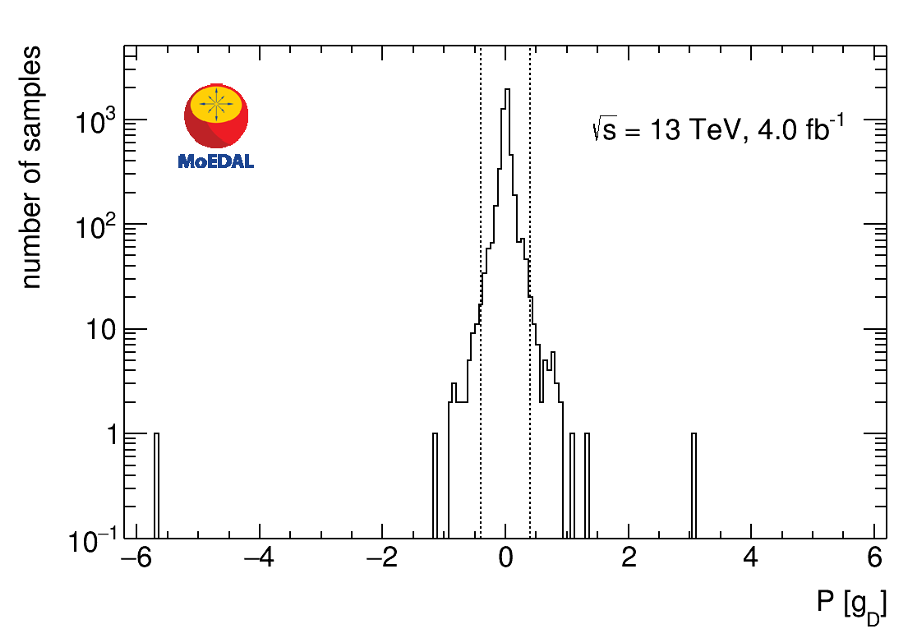
\includegraphics[scale=0.4]{squidanalysis.png}
    \caption{MoEDAL SQUID analysis results: Magnetic pole strength (in units of Dirac charge, $g_D$) measured through the induced persistent current in the 2,400 aluminum of the trappers, exposed to 13 TeV pp collisions in 2015–2017 with every sample scanned twice. From \cite{MoEDAL2017}.}
    \label{squidanalysis}
\end{figure}
\subsubsection{Monopoles and dyons in DY and photon fusion processes}
 MoEDAL has conducted extensive searches assuming conventional perturbative production mechanisms—namely, DY and photon fusion in proton-proton collisions at $\sqrt{s} = 13\text{ TeV}$. Utilizing the aforementioned techniques, the collaboration has placed upper limits on the production cross-section $\sigma$ for monopoles carrying varying magnetic charges (from $1g_D$ up to $6g_D$) and spins ($0, 1/2$, and $1$). Depending on the assumed spin and production kinematics, these non-observations translate into model-dependent lower mass bounds, typically excluding monopole masses up to $\mathcal{O}(1-3)\text{ TeV}$ for lower charges, and up to nearly $6\text{ TeV}$ for higher charges. The analysis naturally extends to dyons (particles carrying both magnetic charge $g$ and electric charge $z$). Because the addition of an electric charge dramatically alters the energy loss $-dE/dx$, the expected kinematic trapping profiles are modified, yet the cross-section bounds remain similarly stringent.
 
 \subsubsection{Schwinger-produced monopoles}
 As discussed previously, evaluating monopole production via perturbative Feynman diagrams is theoretically questionable due to the massive magnetic fine-structure coupling. To circumvent this, MoEDAL pioneered the search for monopoles generated via the non-perturbative Schwinger mechanism during Pb-Pb heavy-ion collisions. When heavy ions pass one another without strong nuclear overlap, the spectator protons generate electromagnetic fields reaching up to $B \sim 10^{16}\text{ T}$. These extreme fields are sufficient to induce spontaneous pair creation of magnetic monopoles from the vacuum, with a production rate scaling as $\Gamma \propto \exp(-\pi M_m^2 / g|\boldsymbol{B}|)$. By scanning the trapper arrays exposed to these specific heavy-ion runs, MoEDAL set the world's first experimental limits on Schwinger-produced monopoles, reliably excluding monopole masses up to $\sim 75\text{ GeV}$ for magnetic charges ranging from $1g_D$ to $3g_D$ \cite{MoEDAL2022}. This result is particularly profound, as it constitutes the first robust mass bound free from the inherent theoretical uncertainties of perturbative QED calculations.

 \begin{figure}[ht!]
    \centering 
    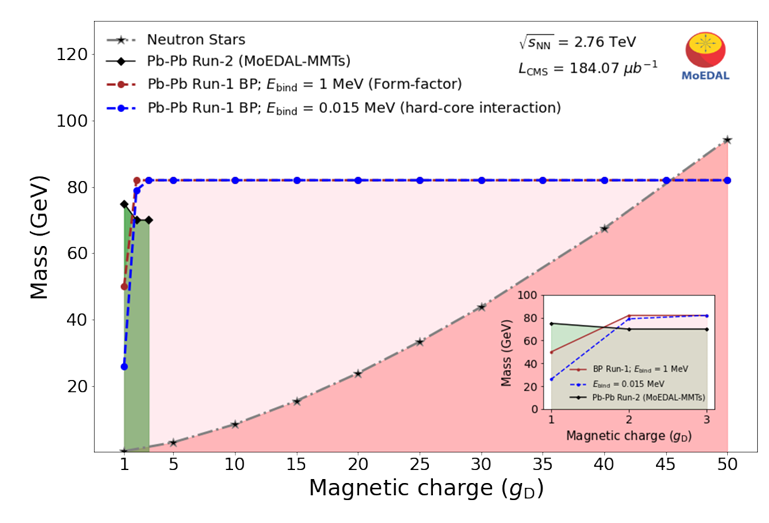
\includegraphics[scale=0.5]{schwingerexclusion.png}
    \caption{Exclusion region for a monopole search via the Schwinger effect in the CMS beam pipe exposed to PbPb collisions during LHC Run 1. The green-shaded region shows the MoEDAL trapper Run-2 limits. The inset zooms in on the lowcharge region. The limit from indirect searches for monopoles produced by neutron stars is also shown. From \cite{MoEDAL2022}.}
    \label{schwingerexclusion}
 \end{figure}
 \subsection{Simulation of monopole production}
 To bridge the theoretical frameworks with the experimental limits set by dedicated searches such as the MoEDAL experiment, it is necessary to perform accurate simulations of monopole production. As we previously stated, diagrammatic approaches using effective couplings remain the standard benchmark for interpreting collider data and generating cross-section limits.  In this context, the simulation of DY monopole pair production mechanism, from a proton proton collision and an intermediate photon $\gamma^*$, is performed utilizing the \textsc{MadGraph5} framework, followed by event analysis and visualization in ROOT. To accommodate a magnetic charge within a standard Monte Carlo generator like \textsc{MadGraph}, a custom Universal FeynRules Output (UFO) model must be implemented. This customized model bypasses the standard QED vertex by substituting the fundamental electric charge $e$ with an effective, velocity-dependent magnetic coupling.  
 
 By virtue of the dual mapping $e \mapsto g\beta$, the effective coupling for a monopole of mass $M_m$ and magnetic charge $g = n g_D$ is explicitly modeled as eq. (\ref{runningcoupling}). This $\beta$-dependent modification is crucial for enforcing the correct kinematic behavior near the production threshold, naturally suppressing the cross-section as the invariant mass of the produced pair approaches the total available partonic energy. 
 
 Once the parton-level events are generated in \textsc{MadGraph} (typically exported as Les Houches Event (\texttt{.LHE}) files) the output is imported into ROOT to construct and evaluate the kinematic phase space. Given the high value of the monopole mass, the available phase space is heavily restricted. Extracting these kinematic distributions ($p_T$, $\eta$, and $\beta$) via ROOT is essential for defining the acceptance grids of the experiment. By comparing these simulated profiles against the acceptance and ionization thresholds of specialized detectors (such as the nuclear track detectors and the aluminum trapping arrays) experimentalists can accurately translate non-observations into the robust cross-section upper limits and mass exclusion bounds established in the modern literature.

 \subsubsection{\texorpdfstring{$\beta\gamma$}{beta-gamma} Distributions}

 Among the various kinematic observables extracted from the Monte Carlo simulations, the momentum-to-mass ratio $p/m$ (or equivalently, the relativistic factor $\beta\gamma$) is of principal importance. As established in Section \ref{51}, the highly-ionizing energy loss mechanism of a magnetic monopole passing through matter is inherently dependent on its velocity. Therefore, accurately mapping the expected $\beta\gamma$ spectra at the production level is a necessary step before passing the generated events through detailed detector simulations (such as GEANT4). The simulated distributions for Drell-Yan spin 1/2 monopole production in $pp$ collisions are presented in Figure \ref{fig:betagamma_distributions}. The grid compares the $\beta\gamma$ spectra for monopoles carrying a fundamental Dirac charge ($1g_D$) against those with double the charge ($2g_D$), across three different masses ($m = 500, 1000,$ and $1500$ GeV). An analysis of these distributions reveals two primary kinematic dependencies:

\begin{itemize}
    \item \textbf{Mass Dependence}: As the monopole mass $M_{\text m}$ increases, the required partonic center-of-mass energy $\hat{s}$ approaches the kinematic limit of the collider. Consequently, heavier monopoles are produced closer to their kinematic threshold, leaving less available energy to be converted into momentum. This is clearly visible traversing the rows of the matrix: for $1g_D$, the mean $\beta\gamma$ drastically drops from $10.26$ at $500$ GeV down to highly non-relativistic regimes of $1.445$ and $1.204$ for $1000$ GeV and $1500$ GeV, respectively.
    \item \textbf{Charge dependence}:  The influence of the magnetic charge on the kinematics is heavily mass-dependent. For lighter monopoles ($500$ GeV), increasing the magnetic charge from $1g_D$ to $2g_D$ severely shifts the spectrum toward lower velocities (the mean drops from $10.26$ to $2.078$). This indicates that the amplified, velocity-dependent effective coupling $g(\beta)$ heavily influences the cross-section integration. However, for heavier monopoles ($1000$ GeV and $1500$ GeV), the charge dependence practically vanishes (means remain $\approx 1.45$ and $\approx 1.20$ regardless of charge). In these high-mass regimes, the phase-space bottleneck and the rapid depletion of the proton's PDFs at high Bjorken-$x$ universally dominate the kinematics, overpowering the dynamical effects of the varying coupling strength.From an experimental standpoint, this confirms that current searches at the TeV scale are inherently hunting for highly non-relativistic, heavily ionizing particles. The sharp peaking of $\beta\gamma \sim \mathcal{O}(1)$ for $M_m \ge 1$ TeV validates the deployment of induction techniques (like SQUIDs) and passive nuclear track detectors, which are optimized precisely for this slow-moving regime.
\end{itemize}

 \begin{figure}[htbp]
    \centering
    
    % Row 1: m = 500 GeV
    \begin{subfigure}[b]{0.48\textwidth}
        \centering
        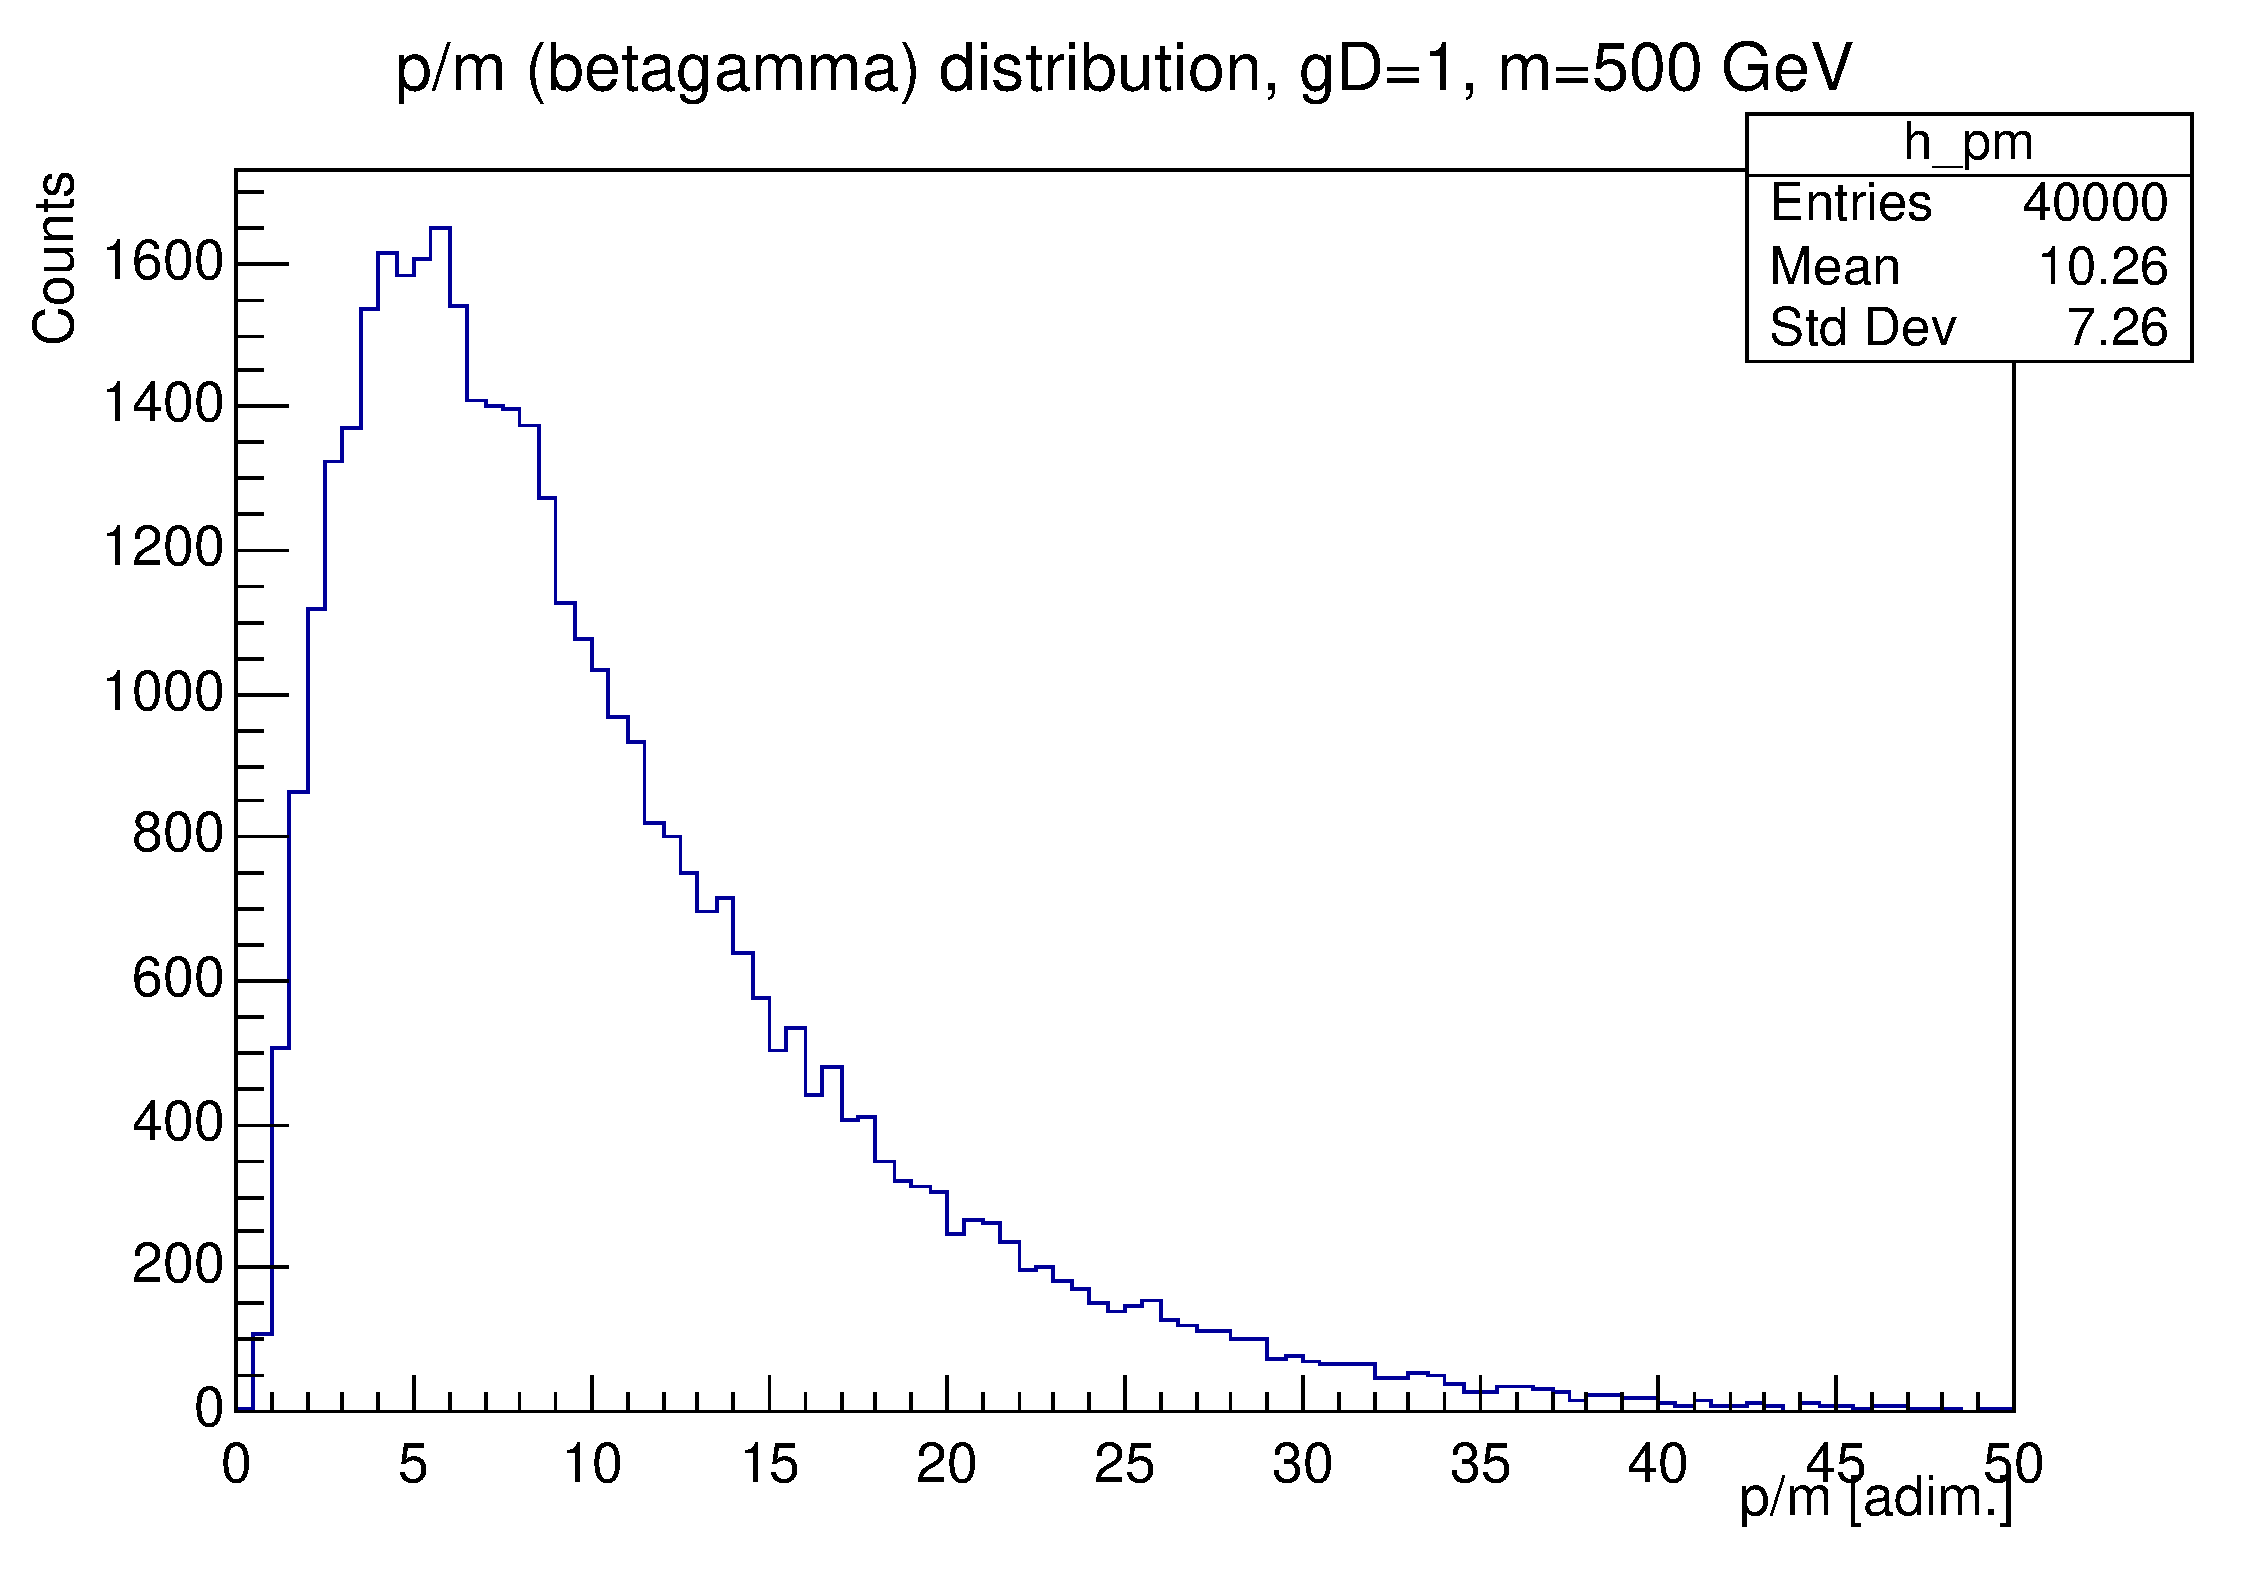
\includegraphics[width=\textwidth]{1.pdf}
        \caption{$m = 500$ GeV, $g = 1g_D$}
        \label{fig:bg_1g_500}
    \end{subfigure}
    \hfill
    \begin{subfigure}[b]{0.48\textwidth}
        \centering
        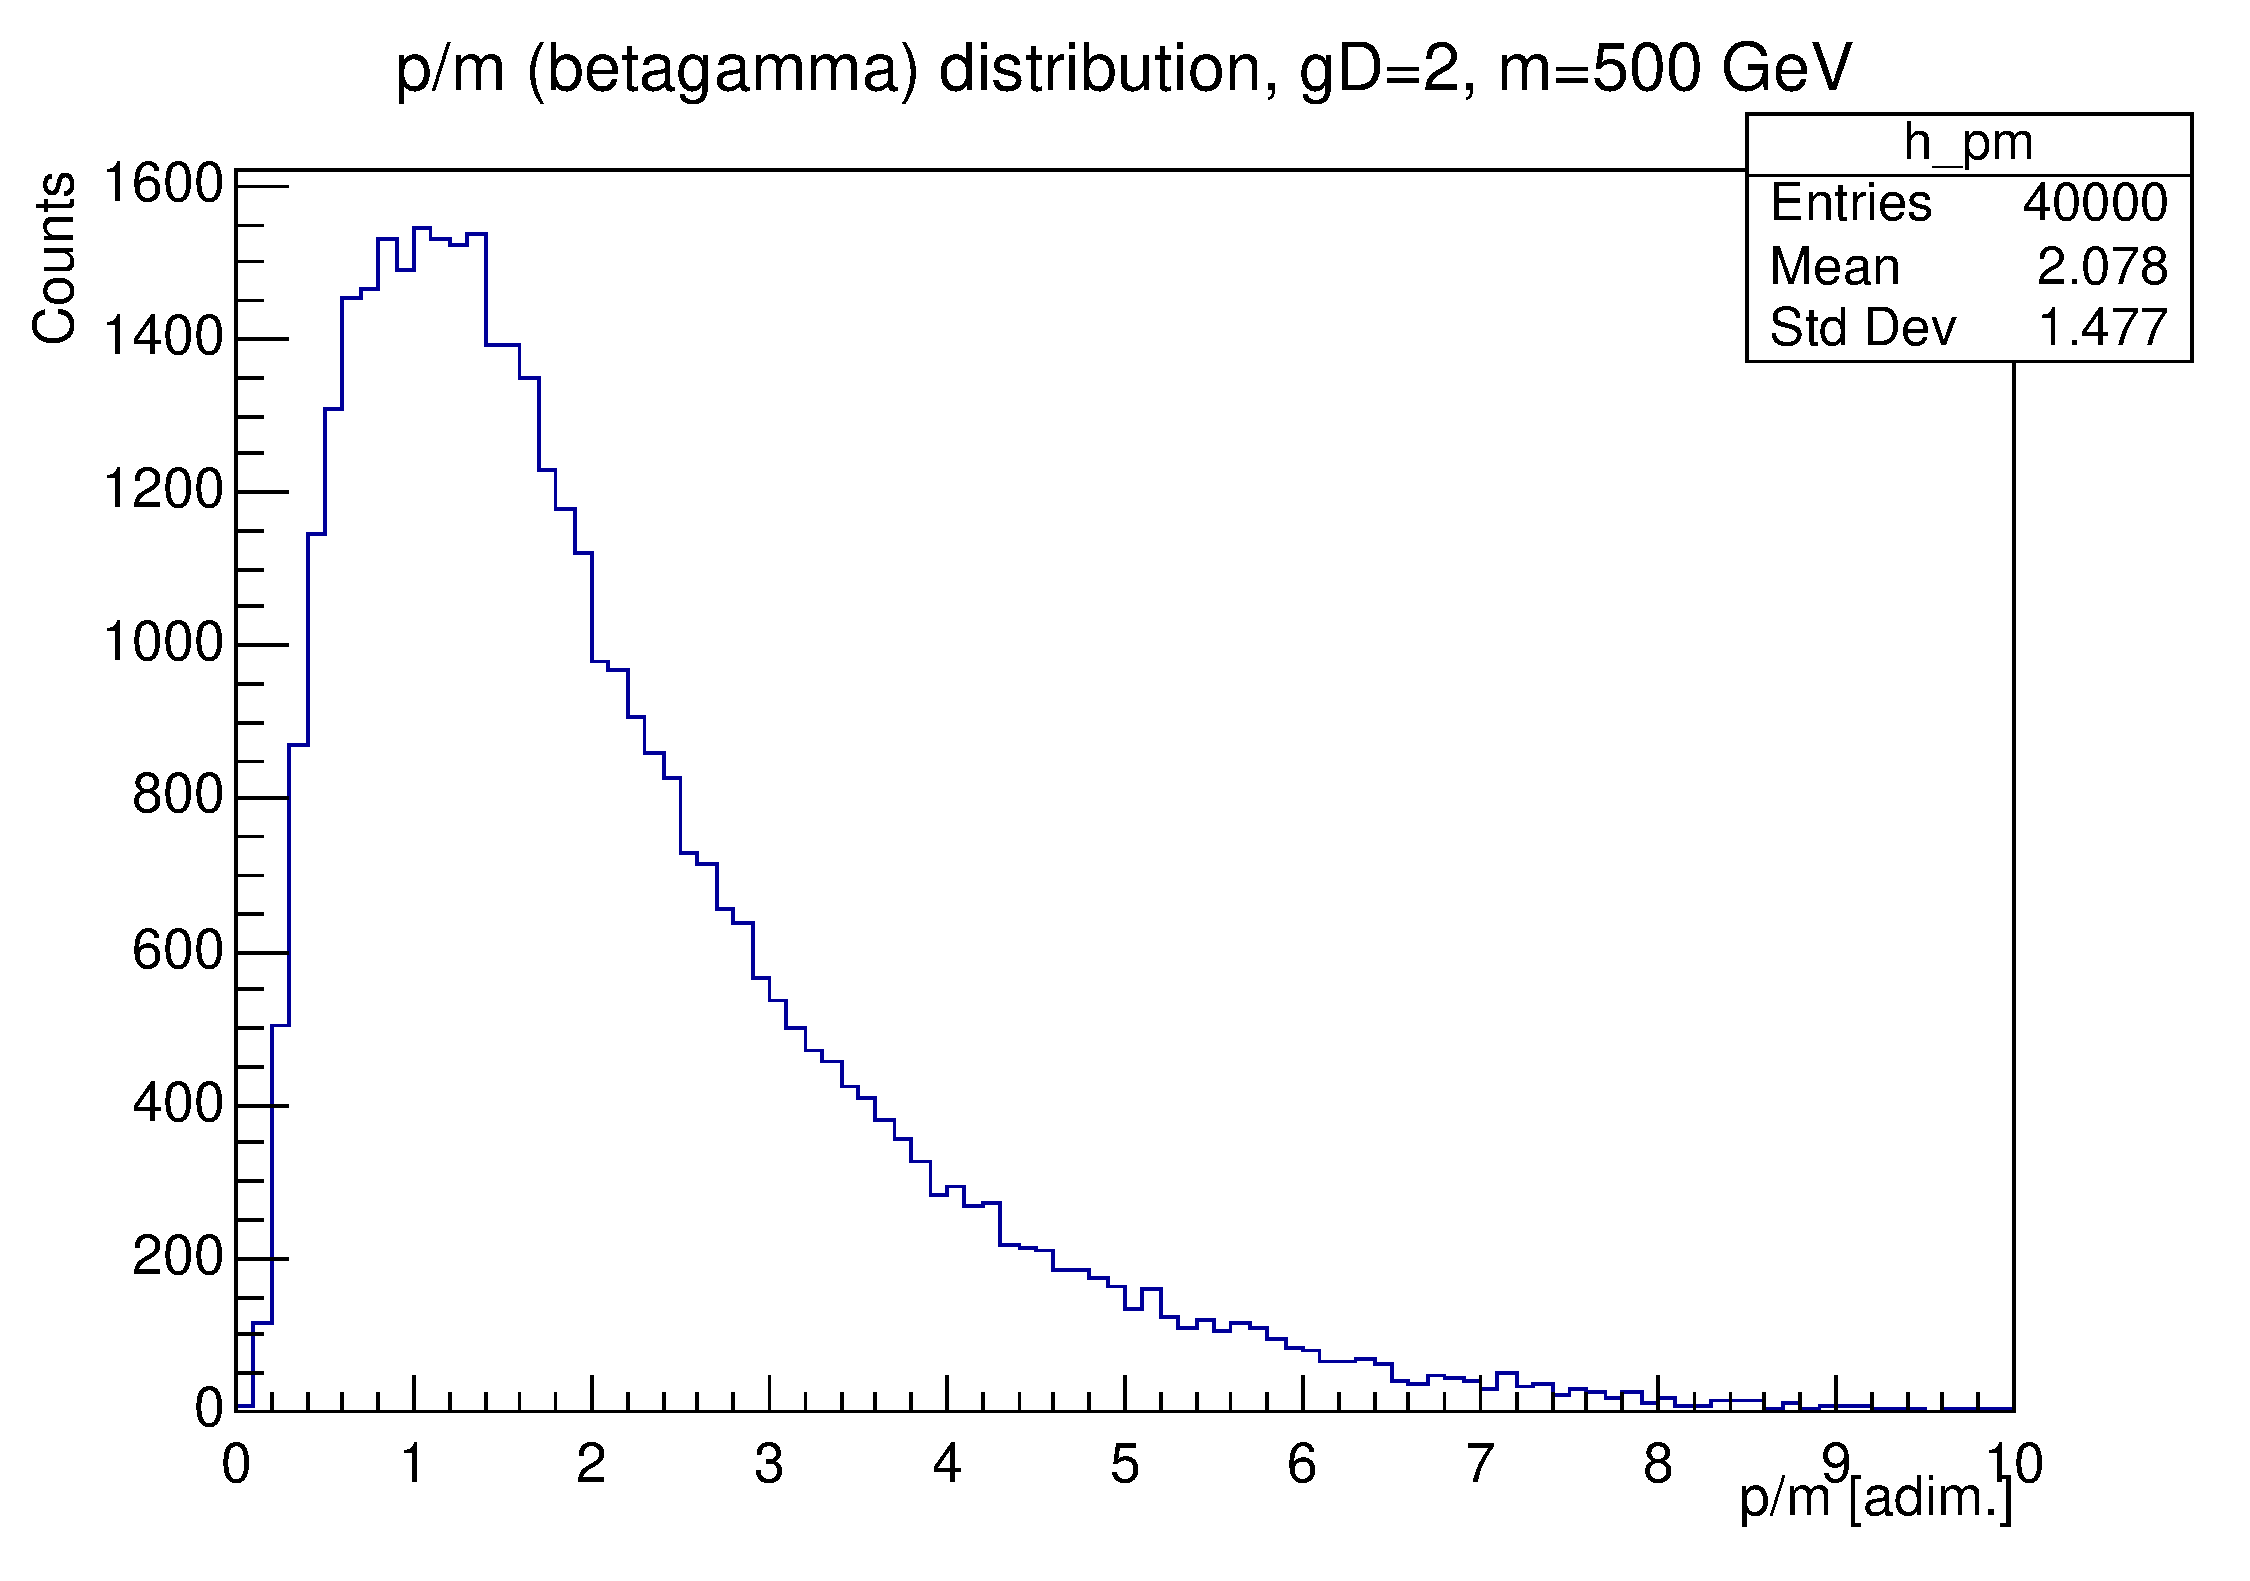
\includegraphics[width=\textwidth]{4.pdf}
        \caption{$m = 500$ GeV, $g = 2g_D$}
        \label{fig:bg_2g_500}
    \end{subfigure}
    
    \vspace{0.5cm} % Vertical spacing between rows
    
    % Row 2: m = 1000 GeV
    \begin{subfigure}[b]{0.48\textwidth}
        \centering
        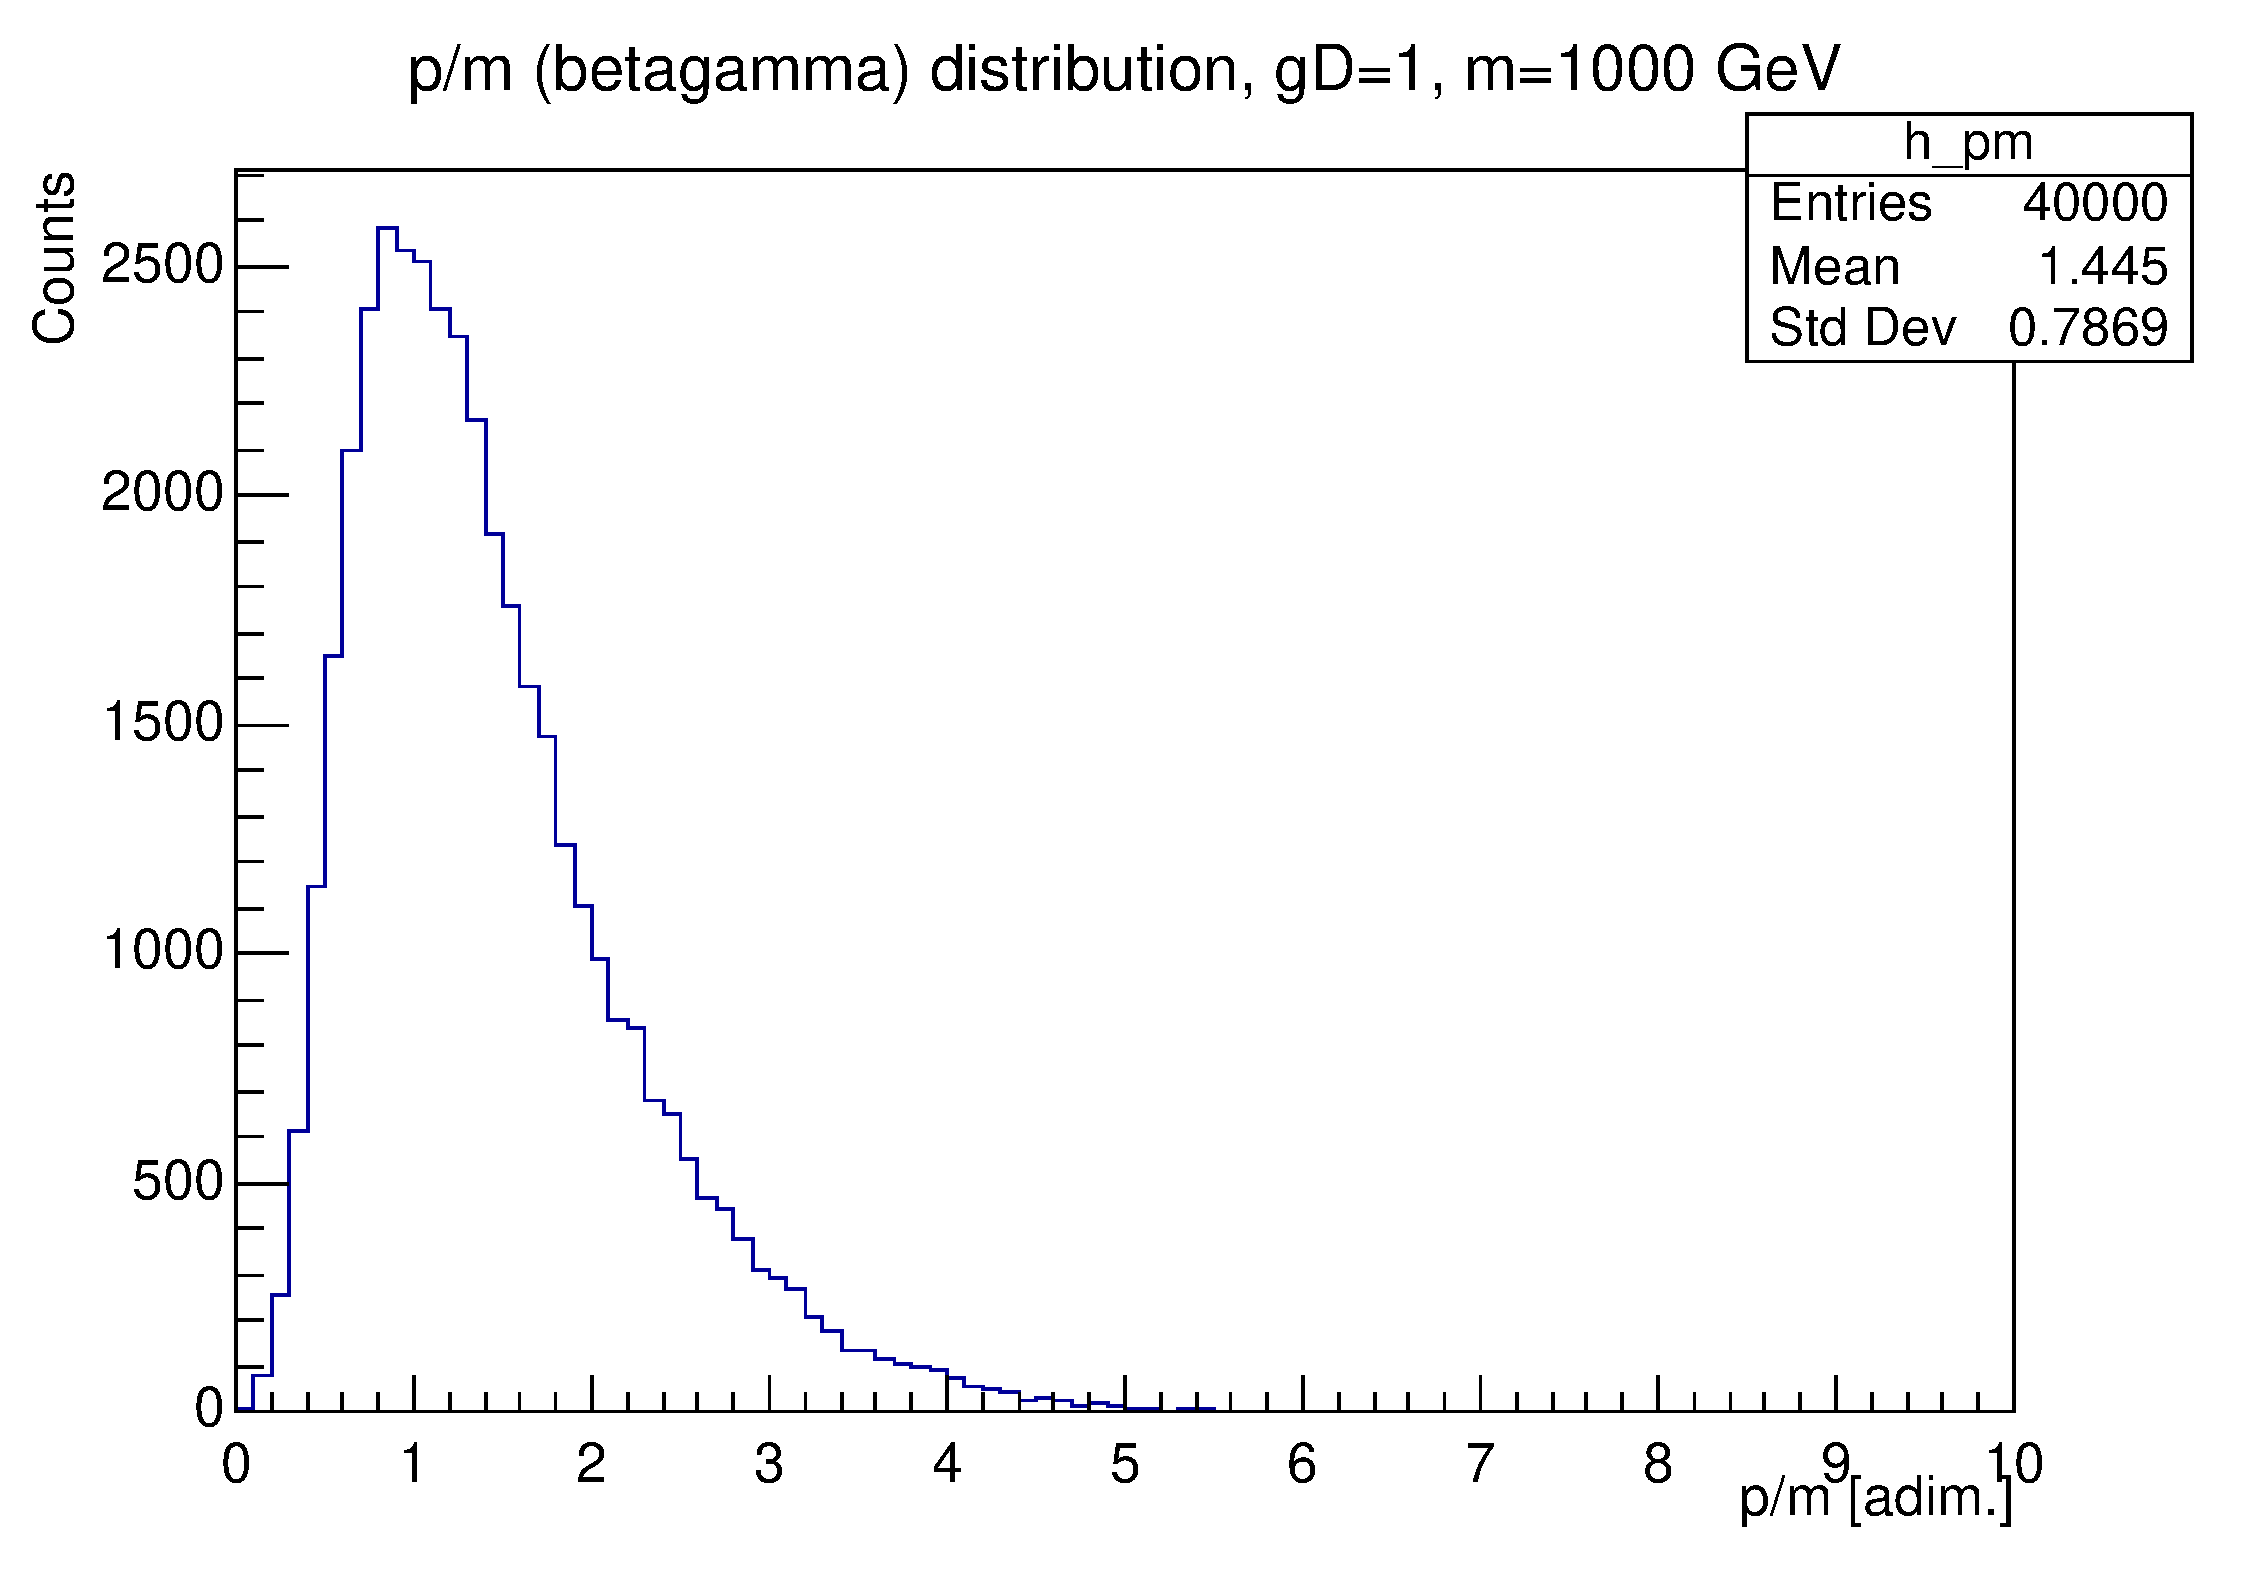
\includegraphics[width=\textwidth]{2.pdf}
        \caption{$m = 1000$ GeV, $g = 1g_D$}
        \label{fig:bg_1g_1000}
    \end{subfigure}
    \hfill
    \begin{subfigure}[b]{0.48\textwidth}
        \centering
        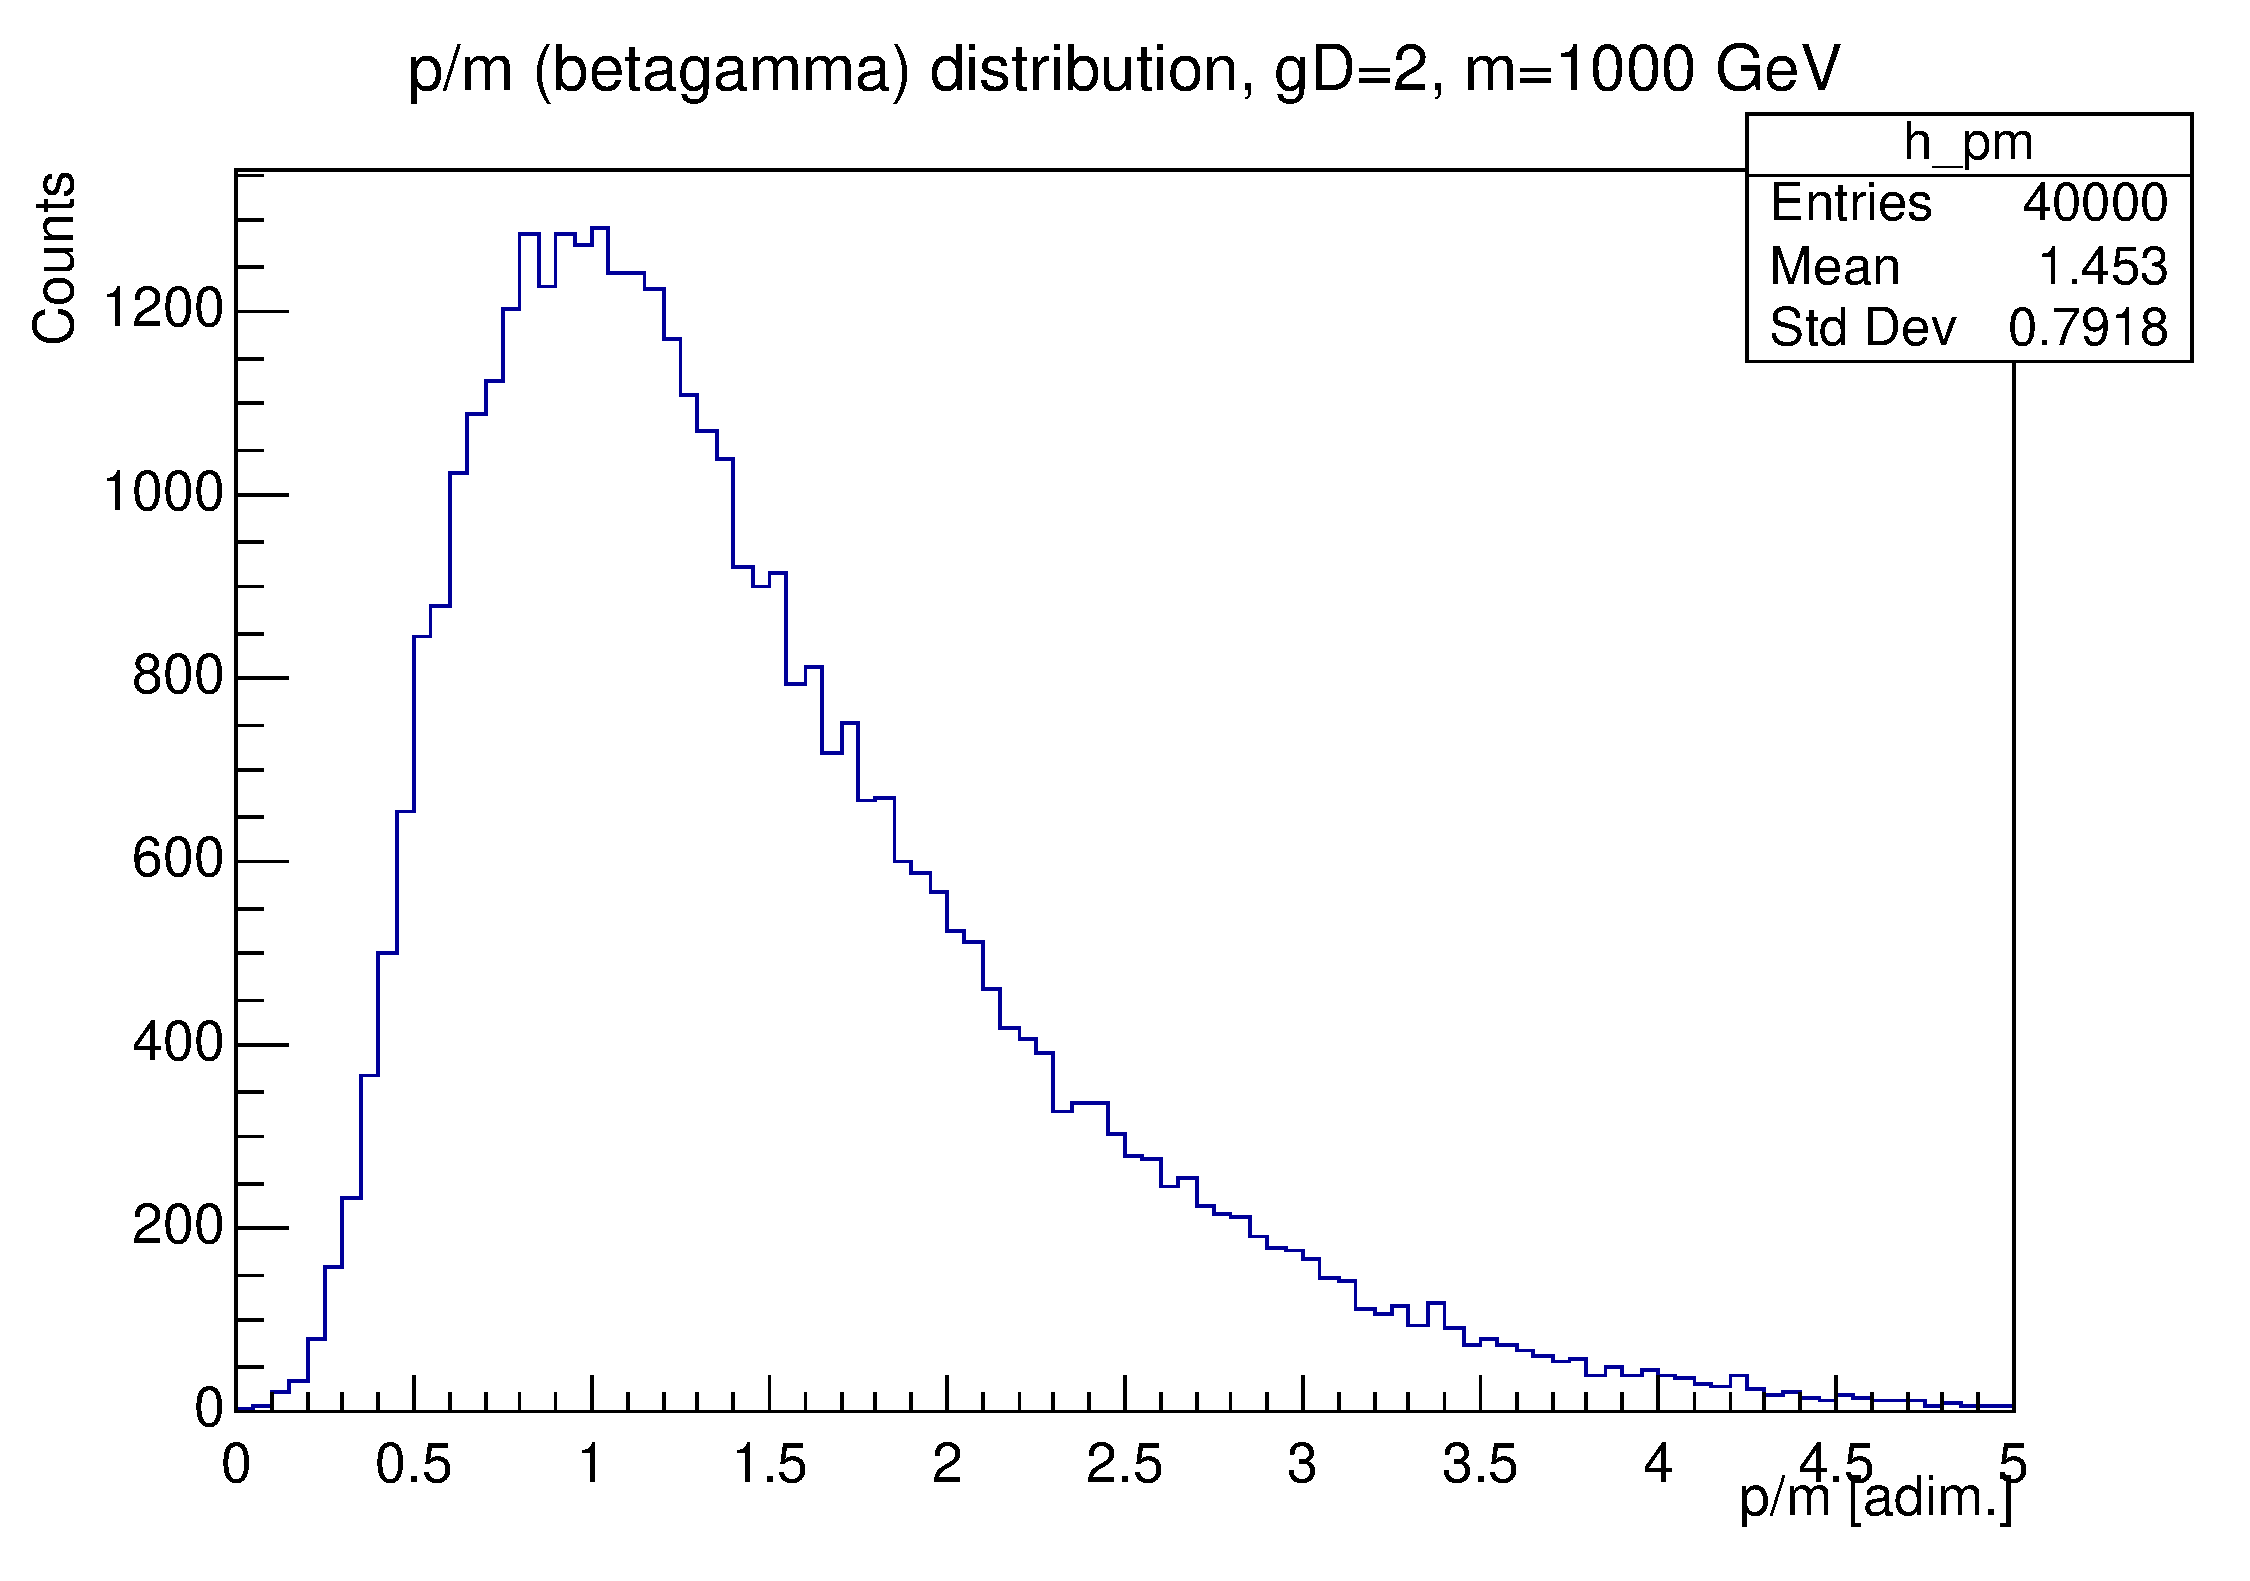
\includegraphics[width=\textwidth]{5.pdf}
        \caption{$m = 1000$ GeV, $g = 2g_D$}
        \label{fig:bg_2g_1000}
    \end{subfigure}
    
    \vspace{0.5cm} % Vertical spacing between rows
    
    % Row 3: m = 1500 GeV
    \begin{subfigure}[b]{0.48\textwidth}
        \centering
        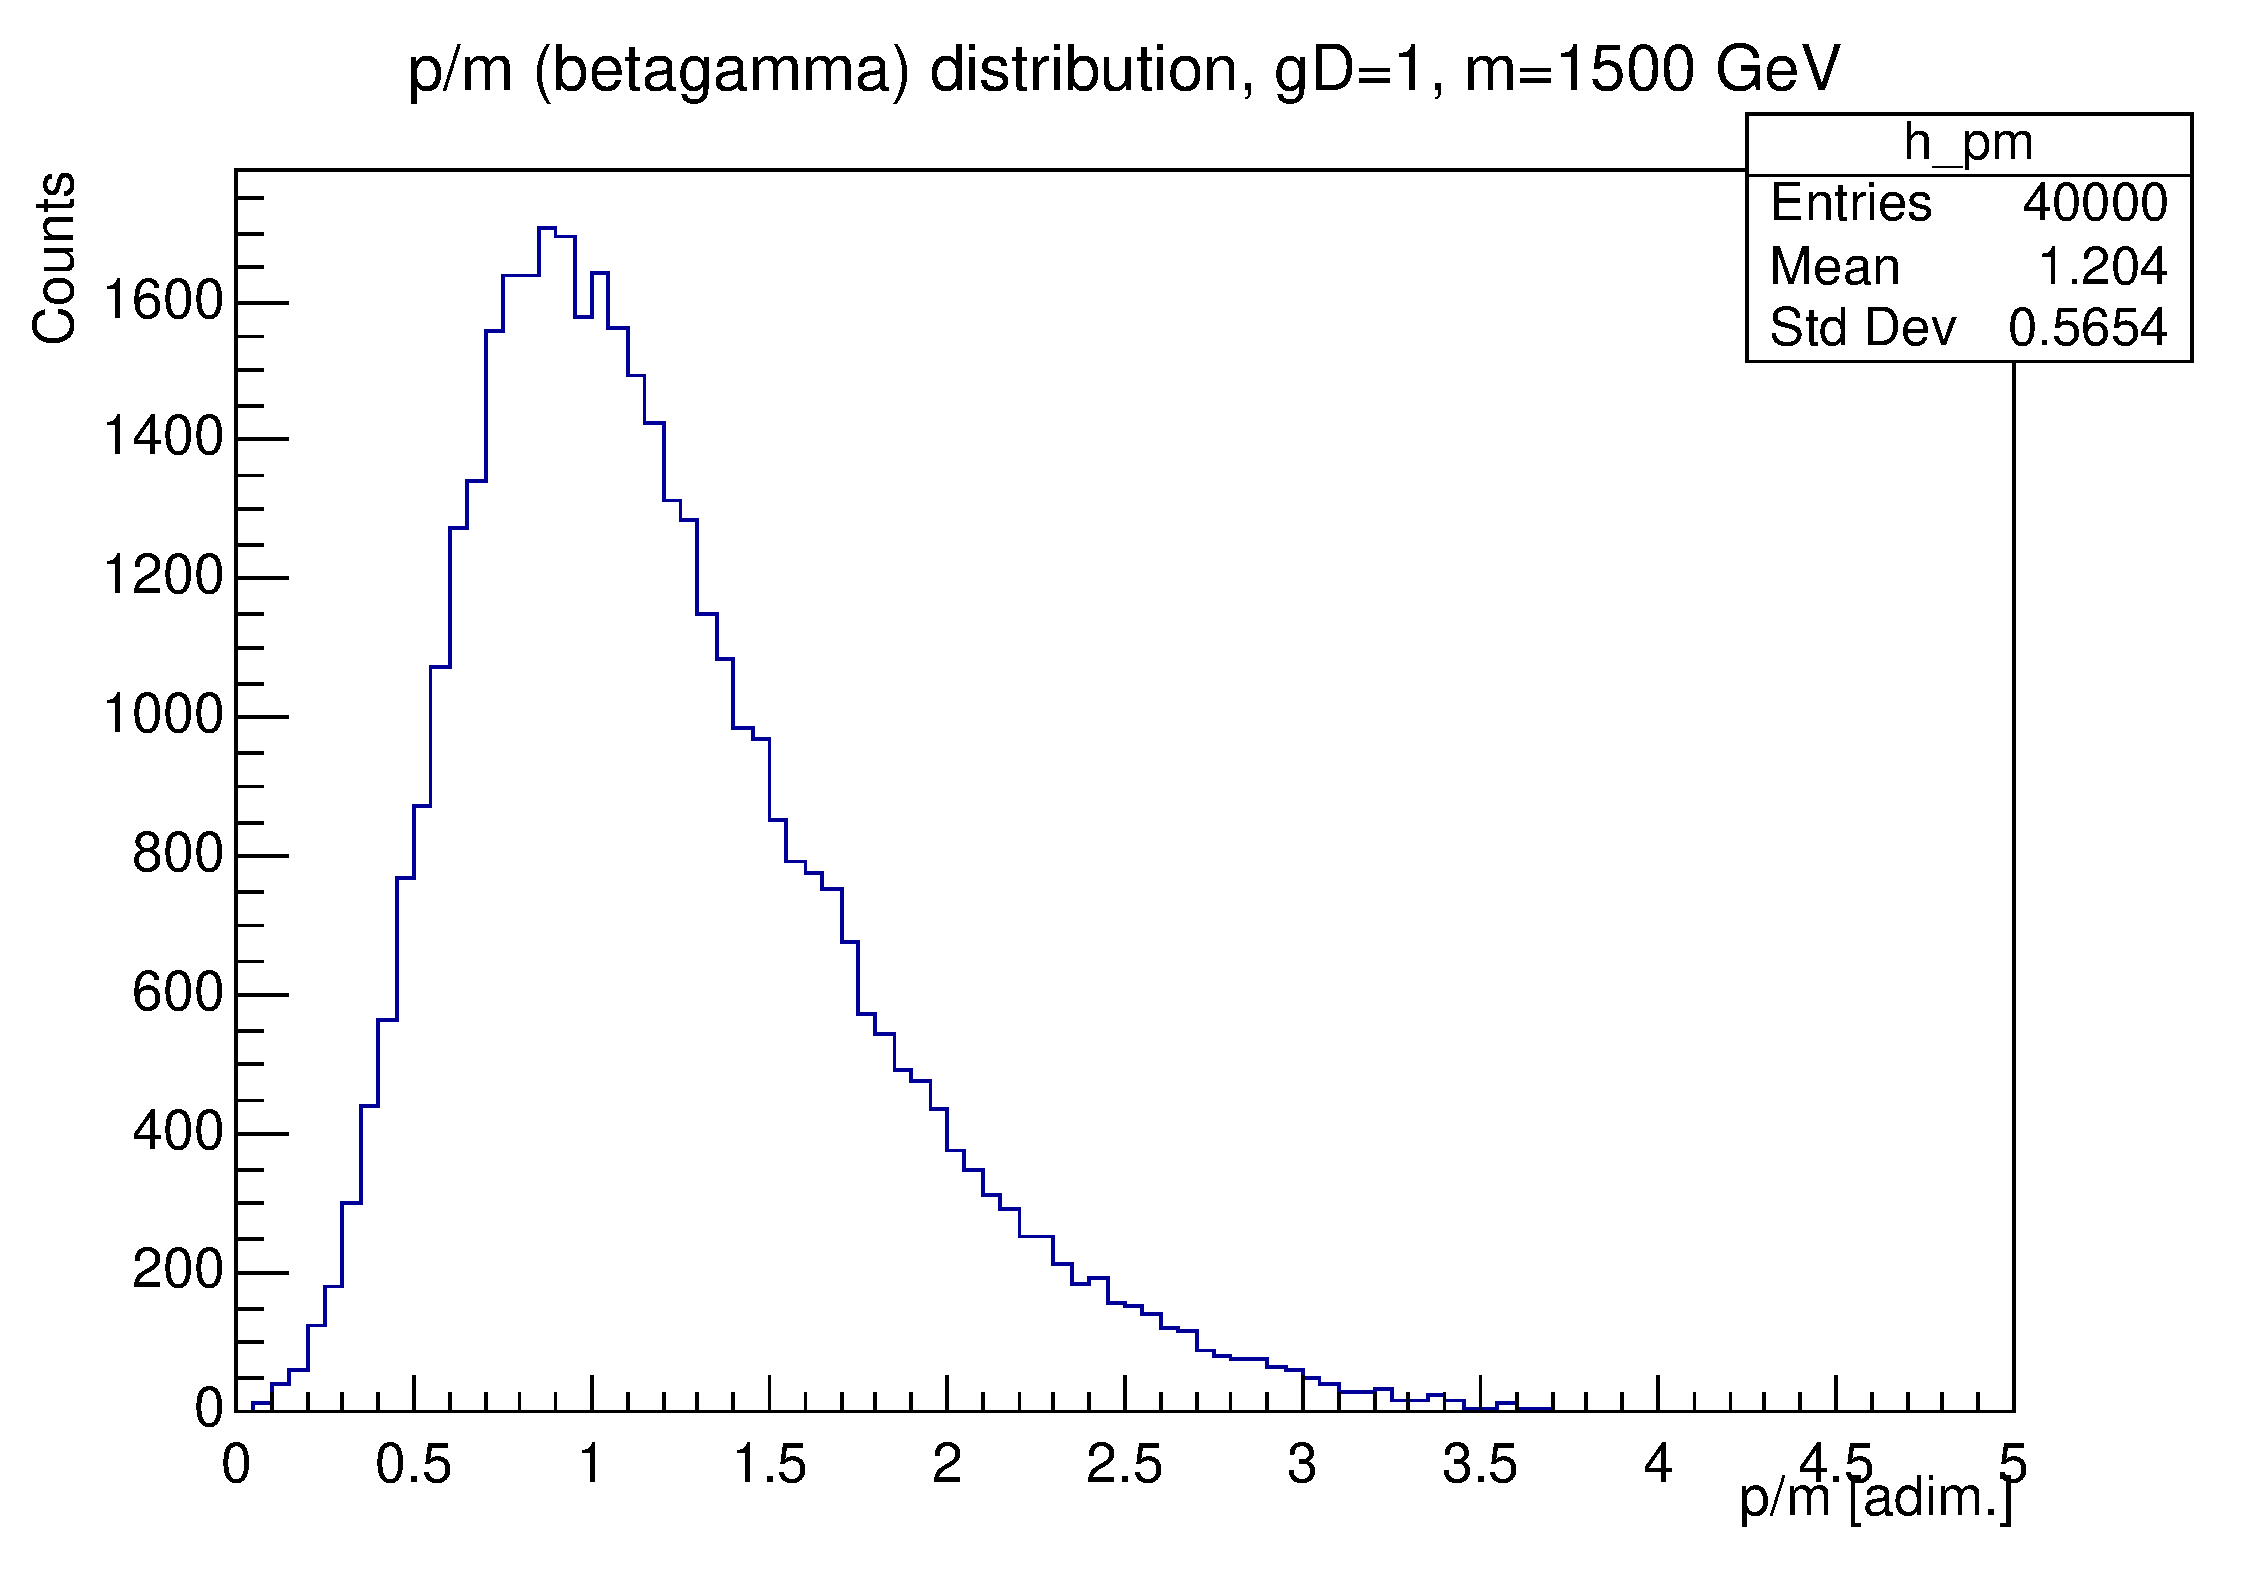
\includegraphics[width=\textwidth]{3.pdf}
        \caption{$m = 1500$ GeV, $g = 1g_D$}
        \label{fig:bg_1g_1500}
    \end{subfigure}
    \hfill
    \begin{subfigure}[b]{0.48\textwidth}
        \centering
        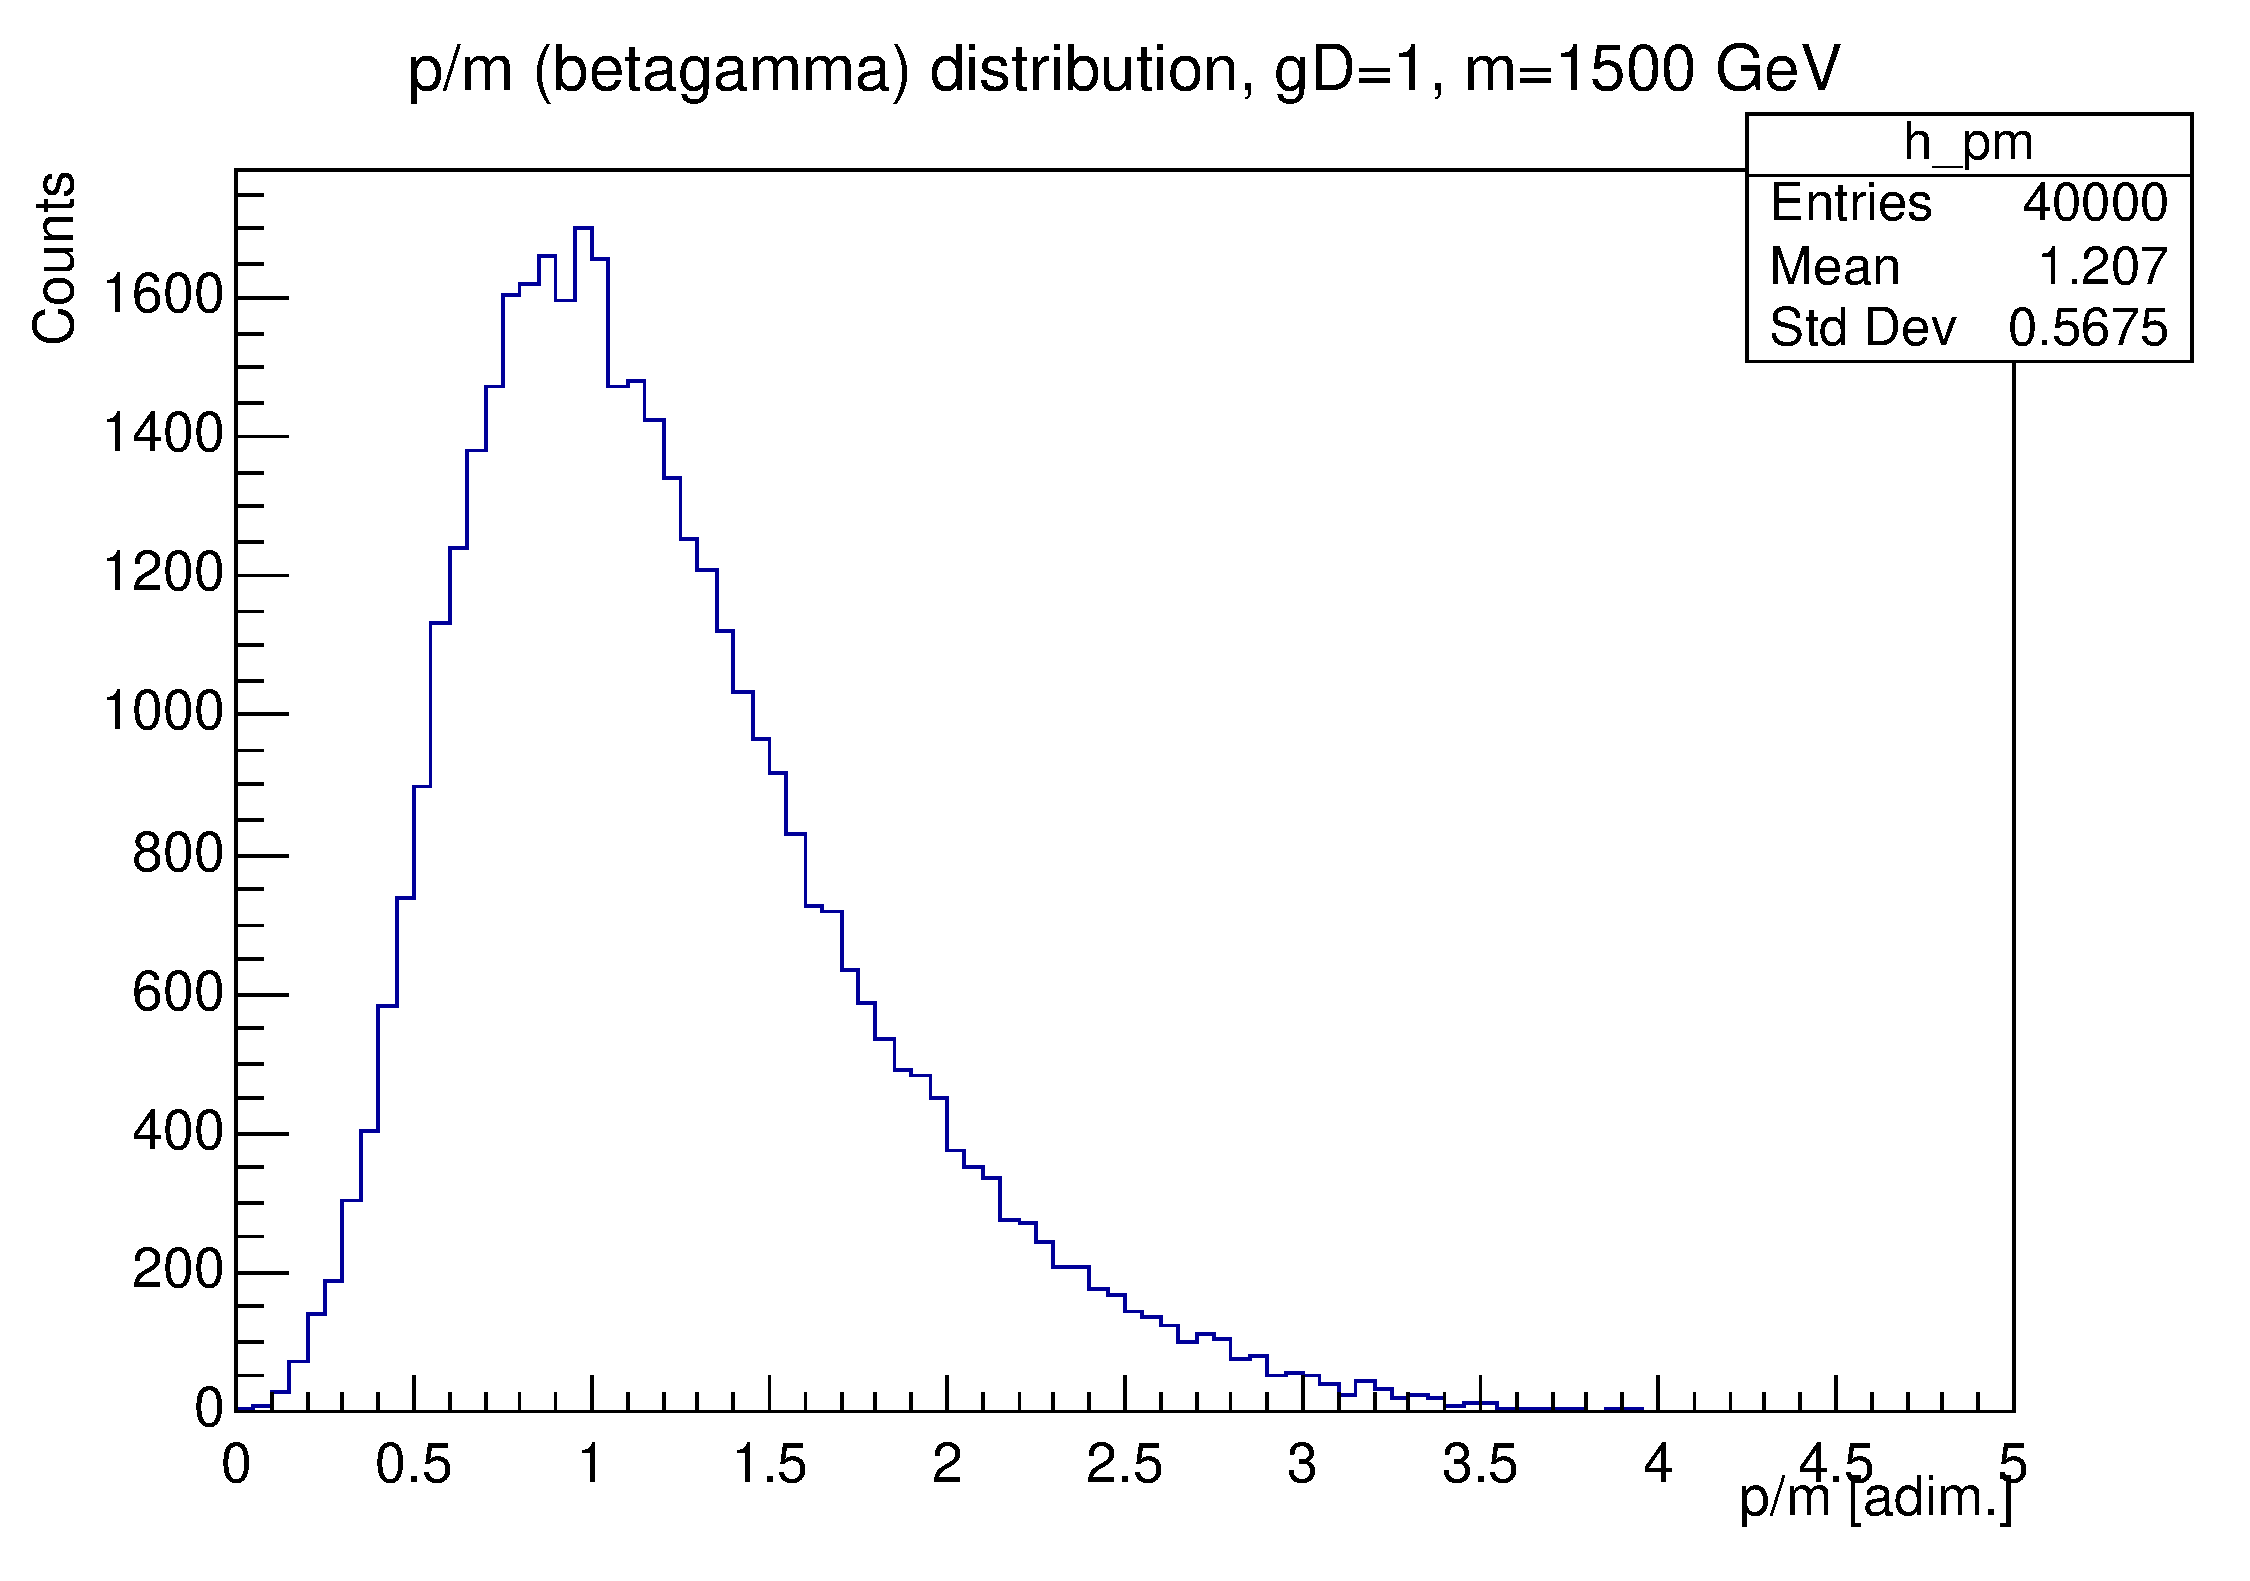
\includegraphics[width=\textwidth]{6.pdf}
        \caption{$m = 1500$ GeV, $g = 2g_D$}
        \label{fig:bg_2g_1500}
    \end{subfigure}
    
    \caption{Simulated $\beta\gamma$ ($p/m$) distributions for magnetic monopoles produced via the Drell-Yan mechanism. The left column corresponds to a fundamental magnetic charge of $1g_D$, while the right column corresponds to $2g_D$. The rows represent different monopole mass hypotheses: $500$ GeV, $1000$ GeV, and $1500$ GeV, illustrating the phase space suppression and coupling dynamics near the production threshold.}
    \label{fig:betagamma_distributions}
\end{figure}

\newpage

% The bibliography will probably be heavily edited during typesetting.
% We'll parse it and, using the arxiv number or the journal data, will
% query inspire, trying to verify the data (this will probalby spot
% eventual typos) and retrive the document DOI and eventual errata.
% We however suggest to always provide author, title and journal data:
% in short all the informations that clearly identify a document.

\begin{thebibliography}{99}

\bibitem{AharonovBohm1959}
Y. Aharonov and D. Bohm, \emph{Significance of electromagnetic potentials in the quantum theory}, \emph{Phys. Rev.} {\bf 115} (1959) 485.

\bibitem{Baines2018}
S. Baines et al., \emph{Monopole production via photon fusion and Drell-Yan processes: MADGRAPH implementation and perturbativity via velocity-dependent coupling and magnetic moment as novel features}, \emph{Eur. Phys. J. C} {\bf 78} (2018) 996.

\bibitem{Birkeland1896}
K. Birkeland, \emph{Sur les rayons cathodiques sous l'action de forces magn\'etiques intenses}, \emph{Comptes Rendus Acad. Sci.} {\bf 123} (1896) 492.

\bibitem{blair2010}
Blair, C. D. A., Cherkis, S. A., \emph{One monopole with k singularities}, \emph{J. High Energy Phys.} {\bf 2010} (2010) pg. 127.

\bibitem{Bogomolnyi1976}
E. B. Bogomol'nyi, \emph{Stability of classical solutions}, \emph{Sov. J. Nucl. Phys.} {\bf 24} (1976) 449.

\bibitem{cao2024}
Cao, L., Xu, Y., \emph{Existence of Julia-Zee dyon and 't Hooft-Polyakov monopole with new field strength tensor}, arxiv:2401.08084.

\bibitem{ChoKimYoon2015}
Y. M. Cho and Kyoungtae Kimm, \emph{Finite Energy Electroweak Monopoles}, arxiv:hep-th/9707038.

\bibitem{Dirac1931}
P. A. M. Dirac, \emph{Quantised singularities in the electromagnetic field}, \emph{Proc. Roy. Soc. Lond. A} {\bf 133} (1931) 60-72.

\bibitem{Ellis_2016}
John Ellis, Nick E. Mavromatos and Tevong You, \emph{The price of an electroweak monopole}, \emph{Phys. Lett. B} {\bf 756} (2016) 29–35.

\bibitem{Ellis2017}
J. Ellis, N. E. Mavromatos, and T. You, \emph{Light-by-Light Scattering Constraint on Born-Infeld Theory}, \emph{Phys. Rev. Lett.} {\bf 118} (2017) 261802.

\bibitem{Epele2012}
L. N. Epele, H. Fanchiotti, C. A. Garc\'ia Canal, V. A. Mitsou, and V. Vento, \emph{Looking for magnetic monopoles at LHC with diphoton events}, \emph{Eur. Phys. J. C} {\bf 72} (2012) 2070.

\bibitem{FaddeevKorepin1978}
L. D. Faddeev and V. E. Korepin, \emph{Quantum theory of solitons}, \emph{Phys. Rep.} {\bf 42} (1978) 1-87.

\bibitem{GeorgiGlashow1974}
H. Georgi and S. L. Glashow, \emph{Unity of All Elementary-Particle Forces}, \emph{Phys. Rev. Lett.} {\bf 32} (1974) 438.

\bibitem{Guth1981}
A. H. Guth, \emph{The Inflationary Universe: A Possible Solution to the Horizon and Flatness Problems}, \emph{Phys. Rev. D} {\bf 23} (1981) 347.

\bibitem{julia1975}
Julia, B., Zee, A., \emph{Poles with both magnetic and electric charges in non-Abelian gauge theory}, \emph{Phys. Rev. D} {\bf 11} (1975) pg. 2227.

\bibitem{KiselevSelivanov1989}
V. G. Kiselev and K. G. Selivanov, \emph{On the one-loop mass shift of the 't Hooft-Polyakov monopole}, \emph{Phys. Lett. B} {\bf 226} (1989) 315-317.

\bibitem{Lazarides1980}
G. Lazarides, M. Magg, and Q. Shafi, \emph{Phase Transitions and Magnetic Monopoles in SO(10)}, \emph{Phys. Lett. B} {\bf 97} (1980) 87.

\bibitem{Milton2006}
Kimball A. Milton, \emph{Theoretical and experimental status of magnetic monopoles}, \emph{Rep. Prog. Phys.} {\bf 69} (2006) 1637–1711.

\bibitem{mitsou2026magneticmonopolesdirac}
Vasiliki A. Mitsou, \emph{Magnetic Monopoles -- From Dirac to the Large Hadron Collider}, arxiv:2605.02869.

\bibitem{2016}
The MoEDAL Collaboration, \emph{Search for magnetic monopoles with the MoEDAL prototype trapping detector in 8 TeV proton-proton collisions at the LHC}, \emph{JHEP} {\bf 2016} (2016) 067.

\bibitem{MoEDAL2017}
MoEDAL Collaboration, \emph{Search for magnetic monopoles with the MoEDAL forward trapping detector in 13 TeV proton-proton collisions at the LHC}, \emph{Phys. Rev. Lett.} {\bf 118} (2017) 061801.

\bibitem{MoEDAL2022}
MoEDAL Collaboration, \emph{First search for magnetic monopoles through the Schwinger mechanism}, \emph{Nature} {\bf 602} (2022) 63.

\bibitem{Nakahara2003}
M. Nakahara, \emph{Geometry, Topology and Physics}, CRC Press (2003).

\bibitem{Poincare1896}
H. Poincar\'e, \emph{Remarques sur une exp\'erience de M. Birkeland}, \emph{Comptes Rendus Acad. Sci.} {\bf 123} (1896) 530.

\bibitem{Polyakov1974}
A. M. Polyakov, \emph{Particle spectrum in quantum field theory}, \emph{JETP Lett.} {\bf 20} (1974) 194-195.

\bibitem{prasad1975}
Prasad, M. K., Sommerfield, C. M., \emph{An exact classical solution for the 't Hooft monopole and the Julia-Zee dyon}, \emph{Phys. Rev. Lett.} {\bf 35} (1975) pg. 760.

\bibitem{PrasadSommerfield1975}
M. K. Prasad and C. M. Sommerfield, \emph{An exact classical solution for the 't Hooft monopole and the Julia-Zee dyon}, \emph{Phys. Rev. Lett.} {\bf 35} (1975) 760.

\bibitem{Rubakov1981}
V. A. Rubakov, \emph{Superheavy Magnetic Monopoles and Proton Decay}, \emph{JETP Lett.} {\bf 33} (1981) 644.


\bibitem{doi:10.1126/science.165.3895.757}
Julian Schwinger, \emph{A Magnetic Model of Matter}, \emph{Science} {\bf 165} (1969) 757-761.

\bibitem{Shnir2005}
Y. M. Shnir, \emph{Magnetic Monopoles}, Springer (2005).

\bibitem{tHooft1974}
G. 't Hooft, \emph{Magnetic monopoles in unified gauge theories}, \emph{Nucl. Phys. B} {\bf 79} (1974) 276-284.

\bibitem{WuYang1975}
T. T. Wu and C. N. Yang, \emph{Concept of nonintegrable phase factors and global formulation of gauge fields}, \emph{Phys. Rev. D} {\bf 12} (1975) 3845.

\end{thebibliography}
\end{document}
